\documentclass[11pt,a4paper]{article}
\usepackage[margin=24mm,headheight=14pt]{geometry}
\usepackage[T1]{fontenc}
\usepackage{lmodern,microtype,amsmath,amssymb,amsthm,mathtools}
\usepackage{booktabs,longtable,array,enumitem,xcolor,hyperref,fancyhdr}
\usepackage{tikz,caption,placeins}
\usetikzlibrary{arrows.meta,positioning,calc,fit,shapes.geometric}
\definecolor{chartblue}{HTML}{235B78}
\definecolor{chartgreen}{HTML}{23745A}
\definecolor{chartorange}{HTML}{AD6222}
\tikzset{box/.style={draw=chartblue,rounded corners=3pt,fill=chartblue!5,align=center,font=\small,minimum height=10mm,inner sep=5pt},learn/.style={box,draw=chartgreen,fill=chartgreen!8},free/.style={box,draw=chartorange,fill=chartorange!9},arr/.style={-{Latex[length=2mm]},thick,draw=chartblue}}
\captionsetup{font=small,labelfont=bf}
\hypersetup{colorlinks=true,linkcolor=blue!45!black,citecolor=chartgreen,urlcolor=blue!55!black,pdftitle={Charts for training-data inversion: theory, architectures, and construction}}
\pagestyle{fancy}\fancyhf{}\lhead{Charts for training-data inversion}\rhead{8 September 2026}\cfoot{\thepage}
\setlength{\parindent}{0pt}\setlength{\parskip}{6pt}
\setlist{leftmargin=*,itemsep=3pt,topsep=4pt}
\newcolumntype{Y}[1]{>{\raggedright\arraybackslash}p{#1}}
\theoremstyle{definition}
\newtheorem{theorem}{Theorem}[section]
\newtheorem{proposition}[theorem]{Proposition}
\newtheorem{lemma}[theorem]{Lemma}
\newtheorem{corollary}[theorem]{Corollary}
\theoremstyle{definition}
\newtheorem{definition}[theorem]{Definition}
\newtheorem{correction}[theorem]{Correction}
\newtheorem{example}[theorem]{Counterexample}
\newtheorem{proposal}[theorem]{Proposal}
\newtheorem{limitation}[theorem]{Limitation}
\newtheorem{literature}[theorem]{Literature connection}
\theoremstyle{remark}\newtheorem{remark}[theorem]{Remark}
\newcommand{\R}{\mathbb R}\newcommand{\Prob}{\mathbb P}\newcommand{\E}{\mathbb E}
\newcommand{\HH}{\mathcal H}\newcommand{\XX}{\mathcal X}\newcommand{\col}{\operatorname{col}}
\newcommand{\row}{\operatorname{row}}\newcommand{\rank}{\operatorname{rank}}
\newcommand{\im}{\operatorname{im}}\newcommand{\dist}{\operatorname{dist}}
\newcommand{\diag}{\operatorname{diag}}\newcommand{\tr}{\operatorname{tr}}
\newcommand{\smin}{\sigma_{\min}}\newcommand{\smax}{\sigma_{\max}}
\newcommand{\norm}[1]{\left\lVert #1\right\rVert}
\newcommand{\ip}[2]{\left\langle #1,#2\right\rangle}
\newcommand{\proj}[1]{P_{#1}}
\newcommand{\status}{\textbf{Status: proved under the stated assumptions.}}
\newcommand{\chapterbrief}[3]{%
\par\smallskip\begingroup\setlength{\fboxsep}{9pt}%
\noindent\fcolorbox{chartblue!35}{chartblue!4}{%
\begin{minipage}{\dimexpr\linewidth-2\fboxsep-2\fboxrule\relax}
\textcolor{chartblue}{\textbf{Executive summary}}\par
#1\par\smallskip
\textbf{How to read this chapter.} #2\par\smallskip
\textbf{Notation to keep in view.} #3
\end{minipage}}\endgroup\par\medskip}
\newcommand{\proofidea}[1]{\par\textcolor{chartblue}{\textbf{Idea before the proof.}} #1\par}
\DeclareMathOperator*{\argmin}{arg\,min}
\begin{document}
\begin{center}
{\LARGE\bfseries Charts for training-data inversion}\\[5pt]
{\large A reader's guide to the theory and to practical chart construction}\\[5pt]
{LoRA certificates, multilayer recovery, and subject-conditioned image atlases}\\[4pt]
Revised and integrated: 8 September 2026
\end{center}

\section*{Executive summary}
\addcontentsline{toc}{section}{Executive summary}

\textbf{The problem.} A released LoRA adapter imposes constraints on the representations of its training data. Those constraints can leave many plausible images unresolved. The goal is to understand when a public model of the candidate family makes inversion identifiable, stable, and computationally manageable.

\textbf{The proposed device.} Replace an unrestricted image $x$ by $x=G(z)$, where $G$ is a fixed public expansion map and $z\in\R^k$ contains the coordinates being searched. Use several small local charts when one chart cannot cover the family. A large frozen decoder does not add unknown coordinates; any weights, noise, or conditioning optimized during inversion do.

\textbf{The central test.} Let $F$ be the chosen observation residual: certificate, replay, gradient matching, or a justified stationarity identity. At a true candidate, define
\[
J=D(F\circ G),\qquad \alpha=\sigma_{\min}(J).
\]
Full column rank and $\alpha>0$ give a stable \emph{local} inverse. The error bound combines chart mismatch, observation error, and inverse conditioning (Theorem~\ref{thm:robust}). The latent dimension $k$ matters through coverage and the actual Jacobian, not through an equation count alone.

\textbf{What the certificate adds.} Write $\HH$ for the private feature span, $q=\dim\HH$, and $p=r-q$ for certificate rank under the exact assumptions. For a fixed smooth $k$-dimensional feature chart with $k<p$, its certified points are exactly its intersection with $\HH$, almost surely over initialization for that fixed chart and span. This removes random-kernel aliases, \emph{not} unwanted span points. Individual recovery requires the chart to meet the span only at the intended points. Polynomial and quadratic expansion families give explicit cases where this is proved.

\textbf{The construction worth pursuing.} Reuse a frozen public decoder; organize subject-relevant local latent patches into a multiscale atlas; use valid certificate lower bounds to prune branches; and optimize the surviving patches. Additional layers or replay help only when they resolve remaining directions with adequate conditioning and justified error models.

\textbf{What is not yet established.} There is no proved universal latent dimension for natural images, no demonstration here that a realistic low-dimensional public atlas covers private photographs, and no generic guarantee of efficient global search. A recognizable or sharper generated image is not evidence that its details belonged to the private example.

\textbf{Status and contribution.} The note contains conditional theorems with full proofs, explicit counterexamples, and labeled construction proposals. Generative-prior inversion, neural atlases, and multiscale geometric approximation already have literature precedents. The research opportunity is their interaction with LoRA's specific information and ambiguity. No numerical experiments or numerical research results are claimed.

\clearpage
\section*{Reader's map and working notation}
\addcontentsline{toc}{section}{Reader's map and working notation}

Each chapter opens with a summary, reading route, and notation guide. Proof statements use upright text. Technical corrections are collected at the end in Appendix~\ref{app:corrections}; each result still states its operative assumptions.

\textbf{Reading routes.} Chapters 1--3 develop the rank and stability theory; Chapters 4--6 explain promising directions and limits. Chapters 7--10 address architectures, image dimension, and subject refinement. Chapters 11--12 develop the multiscale search and the research programme.

At one adapted layer the map is $h\mapsto W_0h+sBAh$: $W_0$ is frozen, $s>0$ is a fixed scale, $A\in\R^{r\times n}$, and $B\in\R^{m\times r}$. The released pair is $(A_T,B_T)$; the attacker knows the frozen backbone and public data, but not the initial $A_0$, private data, or training recipe.

\begin{center}
\small
\begin{tabular}{@{}Y{.25\textwidth}Y{.65\textwidth}@{}}
\toprule
Symbol & Meaning used throughout\\\\
\midrule
$x,\ z,\ G(z)$ & An image, its $k$ searched coordinates, and a public image chart\\\\
$h=\Phi^0(x),\ \psi(w)$ & A frozen layer feature and a direct feature chart\\\\
$H,\ \HH,\ q$ & Private feature matrix, its column span, and that span's rank\\\\
$r,\ p=r-q$ & LoRA rank and exact certificate rank; $q<r\le n$ is assumed for that model\\\\
$C=P_{\row(B_T)^\perp}A_T$ & Computable certificate, with its exact rank and kernel identities assumed where used\\\\
$F,\ J,\ \alpha$ & Observation residual, its derivative on the chart, and smallest singular value\\\\
$\delta,\ \eta$ & Representation error and an allowed observation/residual error\\\\
\bottomrule
\end{tabular}
\end{center}

The score $R(h)=\norm{Ch}^2/\norm{A_Th}^2$ is used only when $A_Th\ne0$. Residual zero-set statements use $Ch=0$ directly. Gaussian laws concern the specified kernel experiment, not arbitrary conditioning on a successful training run. Every optimized nuisance variable belongs in the analysis.

\begin{figure}[htbp]
\centering
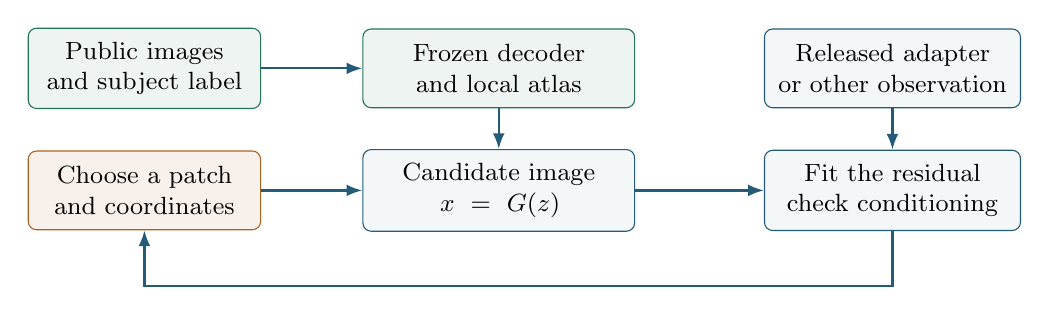
\begin{tikzpicture}
\node[learn,text width=2.6cm] (public) at (0,0) {Public images\\and subject label};
\node[learn,text width=3.1cm] (atlas) at (4.5,0) {Frozen decoder\\and local atlas};
\node[box,text width=2.9cm] (release) at (9.5,0) {Released adapter\\or other observation};
\node[free,text width=2.6cm] (code) at (0,-1.55) {Choose a patch\\and coordinates};
\node[box,text width=3.1cm] (image) at (4.5,-1.55) {Candidate image\\$x=G(z)$};
\node[box,text width=2.9cm] (test) at (9.5,-1.55) {Fit the residual\\check conditioning};
\draw[arr] (public) -- (atlas);
\draw[arr] (atlas) -- (image);
\draw[arr] (release) -- (test);
\draw[arr] (code) -- (image);
\draw[arr] (image) -- (test);
\draw[arr] (test.south) -- ++(0,-.7) -| (code.south);
\end{tikzpicture}
\caption{Two sources with different roles: public data supplies plausible candidates; the released observation supplies evidence. The loop searches candidates but does not manufacture new observations.}
\label{fig:overview}
\end{figure}
\FloatBarrier
\clearpage
\begingroup\small\setlength{\parskip}{0pt}
\tableofcontents
\endgroup
\clearpage

\section{A chart as a general device for inversion}\label{sec:master}

\chapterbrief
{A chart helps when changes in its coordinates produce distinguishable changes in the observation. Full derivative rank gives a stable local solution; the smallest singular value controls how errors are amplified. More restrictive charts can improve sensitivity but miss the true image.}
{First understand the local theorem and its error bound. Then compare image and feature charts, combine two observations, and allow unknown seed or recipe variables. The final proposition instantiates the same machinery for four inversion methods.}
{$G:\R^k\to\XX$ generates candidates; $F:\XX\to\R^a$ is a residual; $J=D(F\circ G)$ and $\alpha=\sigma_{\min}(J)$. A fiber means the set of candidates producing the same observation.}

\subsection{A local inverse means that no small direction is invisible}

\begin{definition}[Objects and conventions]
Let $\XX$ be an open subset of $\R^D$; $D$ is the ambient dimension. A point of $\XX$ may be one input or an ordered tuple of inputs. Let $F:\XX\to\R^a$ be a differentiable observation residual, already centered so that $F(x_*)=0$ at the true object $x_*$. The integer $a$ is its output dimension. A chart is a differentiable map $G:\Omega\to\XX$, where $\Omega\subset\R^k$ is open. Put $f=F\circ G$. All norms are Euclidean or their induced operator norms. For a matrix with at least as many rows as columns, $\smin$ denotes its smallest singular value, including zero. A chart is an immersion at $z$ if $DG(z)$ has column rank $k$. We distinguish isolation of a latent parameter from isolation of its image; a noninjective parameterization can repeat the same image.
\end{definition}

\begin{theorem}[Master local inversion theorem]\label{thm:master}
Assume $F,G$ are $C^1$, $x_*=G(z_*)$, and set
\[
J=DF(x_*)DG(z_*)\in\R^{a\times k},\qquad \alpha=\smin(J).
\]
If $\alpha>0$, there is a convex neighborhood $U$ of $z_*$ such that
\begin{equation}\label{eq:bilip}
\norm{f(z)-f(w)}\ge\frac\alpha2\norm{z-w}\quad(z,w\in U).
\end{equation}
In particular $z_*$ is the only zero in $U$, and an observed residual of size $\eta$ gives a latent error at most $2\eta/\alpha$ there. Conversely, a bound $\norm{z-z_*}\le K\norm{f(z)}$ near $z_*$ implies $\smin(J)\ge K^{-1}$. If $F,G$ are $C^2$, the Hessian at $z_*$ of $\frac12\norm{f(z)}^2$ is $J^TJ$, so it is positive definite under $\alpha>0$.

If instead $Df$ has constant rank $s$ on a neighborhood of $z_*$, the local zero set is a $C^1$ manifold of dimension $k-s$. Rank deficiency at only one point does not imply such a manifold and does not rule out isolated zeros.
\end{theorem}
\begin{proof}
Continuity of $Df$ gives a convex ball $U$ with $\sup_U\norm{Df-J}\le\alpha/2$. The fundamental theorem of calculus along the segment from $w$ to $z$ gives
\[
f(z)-f(w)=J(z-w)+\int_0^1[Df(w+t(z-w))-J](z-w)\,dt.
\]
The first term has norm at least $\alpha\norm{z-w}$ and the integral at most half that bound. This proves \eqref{eq:bilip}, isolation, and the residual estimate. For necessity, set $z=z_*+tv$ for an arbitrary unit vector $v$, divide the assumed estimate by $|t|$, and let $t\to0$. Then $\norm{Jv}\ge K^{-1}$. Differentiating the squared norm gives the Hessian $J^TJ+\sum_j f_jD^2f_j$, whose second term vanishes at the zero. Finally, the constant rank theorem supplies local coordinates in which $f$ is its first $s$ coordinates followed by zeros, up to invertible coordinate changes. Its zero fiber therefore has $k-s$ free coordinates. Every conclusion uses the stated local regularity; no global optimization claim follows.
\end{proof}

\subsection{What representation error and imperfect observations cost}

The nearest useful chart point may not be the truth. The next result compares a local minimizer with a nearby chart point, then translates the coordinate error back into image error. Its search domain matters: no local estimate chooses the correct distant branch automatically.

\begin{theorem}[Chart error, observation error, and a local search]\label{thm:robust}
Suppose $F(x_*)=0$ but the chart only contains $x_0=G(z_0)$ with $\norm{x_0-x_*}\le\delta$. Assume $F$ is $L_F$-Lipschitz between these two points, and $G$ is $L_G$-Lipschitz on a closed latent ball $K=\overline B(z_0,\rho)\subset\Omega$. Let
\[
J_0=D(F\circ G)(z_0),\quad\alpha=\smin(J_0)>0,\quad
\sup_K\norm{D(F\circ G)-J_0}\le\alpha/2.
\]
Let the implemented residual $\widetilde f$ be continuous and satisfy $\sup_K\norm{\widetilde f-f}\le\eta$. Every minimizer $\widehat z$ of $\norm{\widetilde f}$ on $K$ obeys
\begin{align}
\norm{\widehat z-z_0}&\le\frac{4(L_F\delta+\eta)}\alpha,\label{eq:robustz}\\
\norm{G(\widehat z)-x_*}&\le\delta+\frac{4L_G(L_F\delta+\eta)}\alpha.\label{eq:robustx}
\end{align}
If the right side of \eqref{eq:robustz} is below $\rho$, every such minimizer is interior. These are local estimates. A distance to the whole chart does not locate this ball; when a nearest point is not attained, use any $x_0$ within $\delta+\xi$ and retain $\xi>0$.
\end{theorem}
\begin{proof}
Compactness and continuity give a minimizer. Lipschitz continuity and $F(x_*)=0$ give $\norm{f(z_0)}\le L_F\delta$. Optimality at the comparison point $z_0$ yields
\[
\norm{f(\widehat z)}\le\norm{\widetilde f(\widehat z)}+\eta
\le\norm{\widetilde f(z_0)}+\eta\le L_F\delta+2\eta.
\]
The segment argument in Theorem~\ref{thm:master}, now centered at $z_0$, gives
$\frac\alpha2\norm{\widehat z-z_0}\le\norm{f(\widehat z)-f(z_0)}\le2L_F\delta+2\eta$.
This proves \eqref{eq:robustz}. The triangle inequality and the Lipschitz bound for $G$ prove \eqref{eq:robustx}. The interior assertion follows from the distance bound.
\end{proof}

\begin{proposition}[Dimension helps only through geometry]\label{prop:sectional}
Suppose two immersed charts pass through the same point, with tangent spaces $T_S\subset T_U\subset\R^D$ and dimensions $k_S\le k_U$. Define the intrinsic conditioning
\[
\alpha_F(T)=\inf_{v\in T,\,\norm v=1}\norm{DF(x_*)v}.
\]
Then $\alpha_F(T_S)\ge\alpha_F(T_U)$. If their entire images are nested, $\im G_S\subset\im G_U$, their representation errors satisfy $\delta_U\le\delta_S$. Applied separately, Theorem~\ref{thm:robust} gives
\[
\operatorname{error}_j\le\delta_j+4L_{G_j}(L_F\delta_j+\eta_j)/\alpha_j,
\qquad j\in\{S,U\}.
\]
There is no universal winner, nor a rate depending on $k$ alone. Here a sectional chart means a chart of a specified subset $\XX_c\subset\XX$, with a fixed public condition $c$ such as a declared subject. A false declaration can enlarge $\delta_S$ arbitrarily.
\end{proposition}
\begin{proof}
The unit vectors of $T_S$ form a subset of those of $T_U$, so their infimum is larger. The infimum of distance over a larger image is smaller. The error estimates are direct applications of Theorem~\ref{thm:robust}. Neither inequality compares conditioning at different approximation points or between nonnested tangent spaces; neither bounds the other chart's approximation error. Thus they do not imply an ordering of reconstruction errors. Finally, rescaling latent coordinates rescales $DG$ and its parameter singular values without changing the image. This shows why intrinsic conditioning, or the accompanying $L_G$ factor, is essential.
\end{proof}

\subsection{A feature estimate is an image estimate only with a valid readout}

\begin{theorem}[Image charts and feature charts]\label{thm:feature}
Let $\Phi:\XX\to\R^n$ be a $C^1$ frozen feature map and let $Q:\R^n\to\R^a$ be a feature residual. For an image chart $G$, define $\psi=\Phi\circ G$. Then
\[
D(Q\circ\psi)=DQ(\psi)D\Phi(G)DG.
\]
Suppose $\Phi$ is one-to-one on $\im G$ and has an inverse $D_0$ there with Lipschitz constant $L_D$. Searching $Q\circ\psi$ and searching the image objective $Q\circ\Phi\circ G$ are exactly the same latent problem; feature error $e_h$ gives image error at most $L_De_h$ after exact readout by $D_0$.

Conversely, an independently constructed feature chart $\psi$ admits exact image-side realization through a decoder $D_0$ precisely when $\Phi(D_0(\psi(w)))=\psi(w)$ on its domain. If its image contains points outside $\im\Phi$, no such realization exists.

For an orthonormal tangent basis $U\in\R^{D\times k}$, write $V=D\Phi(x_*)U$. If $V$ has column rank $k$, and $\beta$ is the smallest singular value of $DQ$ restricted to the Euclidean subspace $\col V$, then
\[
\smin(DQ\,V)\ge\beta\smin(V).
\]
If $V$ has a kernel, every feature-only objective loses the corresponding image tangent directions.
\end{theorem}
\begin{proof}
The derivative identity is the chain rule. The two latent objectives agree pointwise by definition. The inverse Lipschitz inequality gives the image error claim. Exact realization is equivalent to the displayed right-inverse identity; it is impossible outside the range of $\Phi$. For the singular-value bound, $Vu\in\col V$, so $\norm{DQVu}\ge\beta\norm{Vu}\ge\beta\smin(V)\norm u$. If $Vu=0$, the same product vanishes, independently of $Q$.
\end{proof}

\subsection{A second objective must see what the first one misses}

\begin{figure}[htbp]
\centering
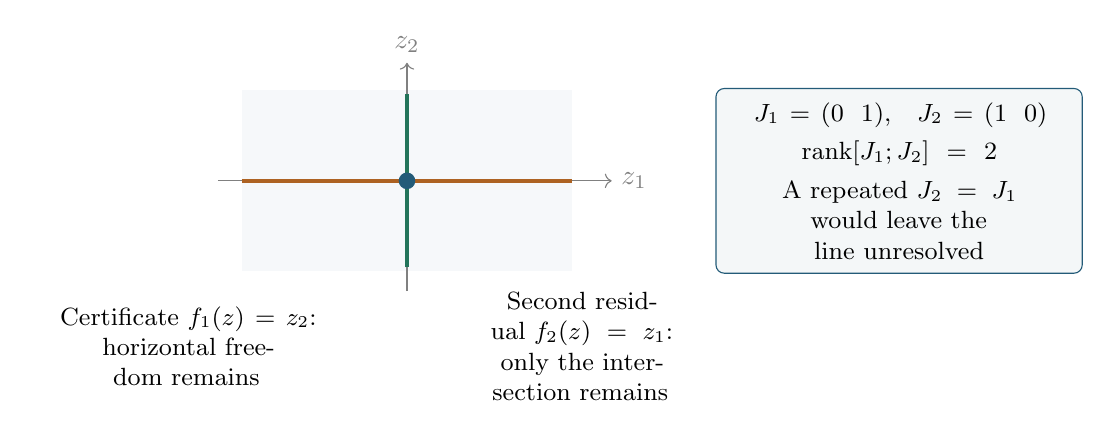
\begin{tikzpicture}[x=1cm,y=1cm]
\fill[chartblue!4] (-2.1,-1.15) rectangle (2.1,1.15);
\draw[->,gray] (-2.4,0) -- (2.6,0) node[right] {$z_1$};
\draw[->,gray] (0,-1.4) -- (0,1.5) node[above] {$z_2$};
\draw[very thick,chartorange] (-2.1,0) -- (2.1,0);
\draw[very thick,chartgreen] (0,-1.1) -- (0,1.1);
\fill[chartblue] (0,0) circle (3pt);
\node[font=\small,align=center,text width=3.8cm] at (-2.8,-2.1) {Certificate $f_1(z)=z_2$:\\horizontal freedom remains};
\node[font=\small,align=center,text width=3.8cm] at (2.2,-2.1) {Second residual $f_2(z)=z_1$:\\only the intersection remains};
\node[box,text width=4.3cm] at (6.25,0) {$J_1=(0\ \ 1)$,\quad $J_2=(1\ \ 0)$\\[3pt] $\rank[J_1;J_2]=2$\\[3pt] A repeated $J_2=J_1$\\would leave the line unresolved};
\end{tikzpicture}
\caption{A two-coordinate example of composition. Complementarity, not a second copy of the first equation, removes the remaining freedom. Theorem~\ref{thm:compose} states the general rank formula and the conditions for a local fiber reduction.}
\label{fig:composition}
\end{figure}
\FloatBarrier

\proofidea{Keep only directions annihilated by the first Jacobian, then test the second Jacobian on those directions. This is why adding all its row counts would overstate its independent contribution. A smooth residual search space requires constant rank nearby, not just a rank value at one point.}

\begin{theorem}[Composition and the residual degrees of freedom]\label{thm:compose}
Let $f_1:\Omega\to\R^{a_1}$ and $f_2:\Omega\to\R^{a_2}$ be $C^1$ residuals vanishing at $z_*$. Write $J_j=Df_j(z_*)$, let $s=\rank J_1$, and let $V\in\R^{k\times(k-s)}$ have orthonormal columns spanning $\ker J_1$. Then
\begin{equation}\label{eq:composition}
\rank\begin{bmatrix}J_1\\J_2\end{bmatrix}
=s+\rank(J_2V).
\end{equation}
Thus the combined residual has a Lipschitz-stable isolated zero if $J_2V$ has column rank $k-s$. If $Df_1$ has constant rank $s$ nearby, $f_1^{-1}(0)$ is locally parameterized by a $C^1$ map $\zeta$ on $\R^{k-s}$, and solving $f_2\circ\zeta=0$ is an exact local reduction. Its conditioning is $\smin(J_2D\zeta)$, with the coordinate metric of $\zeta$ taken into account.

If every exact replay solution in a neighborhood is a certificate solution, imposing the certificate does not change the replay zero set. If in addition the replay derivative has constant rank nearby, the certificate derivative at the truth vanishes on the replay kernel, and its rows belong to the row space of the replay derivative.
\end{theorem}
\begin{proof}
The kernel of the stacked matrix is $\ker J_1\cap\ker J_2=V\ker(J_2V)$. Its dimension is $(k-s)-\rank(J_2V)$, proving \eqref{eq:composition} by rank-nullity. The stable isolation statement follows from Theorem~\ref{thm:master}. Constant rank supplies the local fiber chart $\zeta$; its tangent spans $\ker J_1$, so the chain rule proves the reduced rank criterion. The solution-set assertion is simply $Z_{\rm replay}\cap Z_{\rm cert}=Z_{\rm replay}$ under inclusion. Under constant replay rank, every vector in its derivative kernel is the velocity of a curve of replay zeros. The certificate is zero on that curve, so differentiating annihilates that vector. Orthogonal complements give the row-space inclusion. Without the constant-rank hypothesis, identical zero sets alone do not imply identical derivative ranks.
\end{proof}

\subsection{Unknown training choices can imitate a change in the data}

The nuisance projection below removes observation changes that could be explained solely by adjusting the unknown seed, recipe, or coefficients. Only the part left over can distinguish the data coordinates at first order.

\begin{theorem}[Unknown seed, recipe, or KKT coefficients]\label{thm:nuisance}
Let $f(z,u)\in\R^a$ be a $C^1$ residual with nuisance parameter $u\in\R^t$, and $f(z_*,u_*)=0$. Put $A_z=D_zf$ and $V_u=D_uf$ at that point. Assume $V_u$ has column rank $t$. The joint parameter $(z,u)$ has an injective derivative if and only if
\[
K=(I-\proj{\col V_u})A_z
\]
has column rank $k$. At the linearized level the data directions visible after allowing nuisance changes have rank $\rank K$.
\end{theorem}
\begin{proof}
A vector $(a,b)$ lies in the joint kernel exactly when $A_za+V_ub=0$. This has a solution in $b$ if and only if $Ka=0$, and that solution is unique because $V_u$ is injective. Hence the joint kernel is trivial exactly when $K$ is injective. The same equivalence identifies the linearized invisible data directions as $\ker K$. Theorem~\ref{thm:master} then gives local stable joint inversion. Redundant nuisance coordinates require a justified local gauge reduction; the projection criterion alone is only infinitesimal if that regularity is absent.
\end{proof}

\subsection{The same test for certificate, replay, gradient, and KKT inversion}

\begin{proposition}[The four inversion residuals]\label{prop:four}
The preceding theorems apply to the following precisely defined residuals, on any branch where they are differentiable. Let $X=(x_1,\ldots,x_M)$ denote a data tuple, with labels fixed unless included among nuisance variables. Let $\theta$ denote network parameters and $\ell(\theta;x_i,y_i)$ a differentiable per-example loss.
\begin{enumerate}
\item \emph{Certificate:} $F_C(x)=C\Phi^0(x)$, or its blockwise counterpart for a tuple. It is linear in $h=\Phi^0(x)$ and generally nonlinear in $x$. Its derivative on an image chart is $CD\Phi^0DG$. Under the exact certificate assumptions its construction needs neither $A_0$ nor the recipe.
\item \emph{Replay:} let $\mathcal T(X,u)$ be the released endpoint produced by a fully specified training procedure and let $y$ be the observed endpoint. Set $F_R(X,u)=\mathcal T(X,u)-y$. Here $u$ includes unknown seed, continuous recipe choices, and any other unobserved continuous variables. Known discrete recipes or schedules define separate branches. Its chart derivative is $D_X\mathcal T\,DG$; with unknown $u$, Theorem~\ref{thm:nuisance} applies. This residual is generally nonlinear even in training features.
\item \emph{Gradient matching:} for a known evaluation parameter $\theta_0$ and a released gradient $g$, let $F_\nabla(X)=\sum_i a_i\nabla_\theta\ell(\theta_0;x_i,y_i)-g$, where $a_i$ are known aggregation weights. Its derivative uses mixed input/parameter derivatives. It needs the gradient's evaluation and aggregation specification, not an entire subsequent training trajectory. Unknown labels or weights are additional nuisance variables.
\item \emph{Stationarity/KKT:} for known $b\in\R^a$ and known differentiable per-example map $v(\theta;x,y)\in\R^a$, a candidate stationarity identity is $F_K(X,\lambda)=b-\sum_i\lambda_i v(\theta;x_i,y_i)$. The multipliers $\lambda_i$ are nuisance variables unless given. This is valid only when the relevant stationary/KKT identity and its constraints hold; a finite endpoint need not satisfy it. Inequalities need an active-set or constrained analysis, not just this equality residual.
\end{enumerate}
In every case the independent first-order constraints are the rank of its actual chart derivative, or its nuisance-projected derivative. No universal rank follows from the label of the attack. For the certificate, the sharper rank formula in Theorem~\ref{thm:localcert} is available.
\end{proposition}
\begin{proof}
Each formula defines the residual to which Theorem~\ref{thm:master} applies. The derivatives follow by the chain rule and differentiation of the displayed sums. Eliminating the allowed infinitesimal nuisance changes gives exactly Theorem~\ref{thm:nuisance}. The certificate's special linearity follows from fixing $C$ while varying the candidate. The remaining formulas contain model derivatives or iterated training and have no stated structural assumption forcing a generic rank. For piecewise smooth networks these assertions hold on a fixed differentiable stratum; they do not assert differentiability at activation boundaries.
\end{proof}

\clearpage
\section{The certificate worked case}\label{sec:certificate}

\chapterbrief
{The certificate annihilates the private feature span, not just the training points. A chart can turn that span constraint into individual recovery only when it excludes unwanted span points. Fixed-chart rank and random-matrix results tell us when the remaining directions are identifiable and how stably they can be recovered.}
{Start with the kernel picture and local/global distinction. The explicit expansions show a prior condition that can actually be proved. Affine bias, wrong-chart tests, and conditioning then explain approximate recovery; product charts and candidate tests address multiple examples.}
{$\HH=\col H$ has rank $q$; $p=r-q$ is certificate rank; $b=n-q$ is the dimension outside the private span. The normalized matrix $C_{\rm w}$ has orthonormal rows and the same kernel as $C$.}

\subsection{Separate the private span from the additional invisible directions}

\begin{figure}[htbp]
\centering
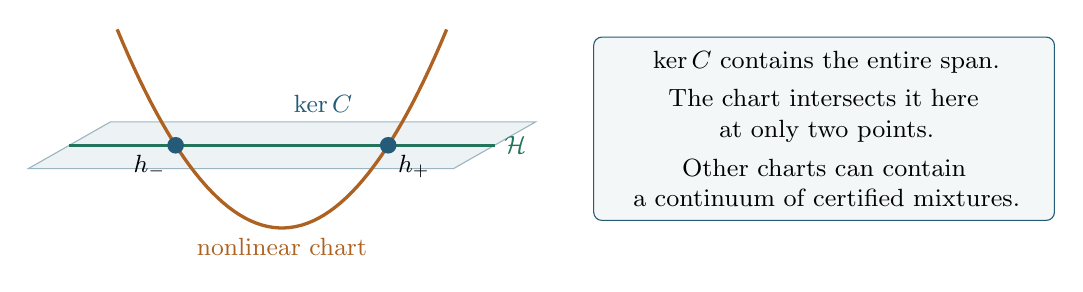
\begin{tikzpicture}[x={(1.35cm,0cm)},y={(.58cm,.33cm)},z={(0cm,1.05cm)}]
\filldraw[fill=chartblue!8,draw=chartblue!45] (-2,-.9,0) -- (2,-.9,0) -- (2,.9,0) -- (-2,.9,0) -- cycle;
\draw[very thick,chartgreen] (-2,0,0) -- (2,0,0);
\draw[very thick,chartorange,domain=-1.55:1.55,samples=60] plot (\x,0,{\x*\x-1});
\fill[chartblue] (-1,0,0) circle (3pt);
\fill[chartblue] (1,0,0) circle (3pt);
\node[font=\small,below left] at (-1,0,0) {$h_-$};
\node[font=\small,below right] at (1,0,0) {$h_+$};
\node[font=\small,chartgreen,anchor=west] at (2,0,0) {$\HH$};
\node[font=\small,chartblue,anchor=south] at (0,.9,0) {$\ker C$};
\node[font=\small,chartorange,anchor=north] at (0,0,-1) {nonlinear chart};
\node[box,text width=5.5cm] at (5.1,0,.2) {$\ker C$ contains the entire span.\\[3pt] The chart intersects it here\\at only two points.\\[3pt] Other charts can contain\\a continuum of certified mixtures.};
\end{tikzpicture}
\caption{An exact geometric example, not a natural-image model: in $\R^3$, let $C$ have rows $(0,0,0)$ and $(0,0,1)$, let $\HH=\operatorname{span}(e_1)$, and use $\psi(t)=(t,0,t^2-1)$. Its residual is $(0,t^2-1)$, so the only zeros are $h_\pm=(\pm1,0,0)$. This illustrates span separation; it does not invoke a generic-rank theorem.}
\label{fig:kernelgeometry}
\end{figure}
\FloatBarrier

\begin{definition}[Certificate geometry and a computable normalization]\label{def:cert}
Fix $H\in\R^{n\times M}$, $\HH=\col H$, $q=\rank H$, and $q<r\le n$. Set
\[
p=r-q,\qquad b=n-q.
\]
Thus $p$ is certificate rank and $b$ is the dimension of the quotient by the private span. Assume the supplied exact identities $\rank C=p$ and $\ker C=\HH\oplus\ker A_0$. For the compact singular value decomposition $C=U_C\Lambda_C V_C^T$, define the observable whitened certificate
\[
C_{\rm w}=V_C^T\in\R^{p\times n}.
\]
It satisfies $C_{\rm w}C_{\rm w}^T=I_p$ and $\ker C_{\rm w}=\ker C$. Its basis is immaterial: the invariant score is
\[
\norm{C_{\rm w}h}^2=h^T C^\dagger C h.
\]
Here $C^\dagger$ is the Moore--Penrose inverse. Whitening changes nonzero objective values and conditioning; it preserves the zero set. It is useful because the kernel theorem alone does not specify the scale or singular values of $C$.
\end{definition}

\begin{lemma}[The quotient experiment implied by the kernel]\label{lem:quotient}
Let $Q_0\in\R^{n\times q}$ and $Q_1\in\R^{n\times b}$ be fixed orthonormal bases of $\HH$ and $\HH^\perp$. Suppose $A_0$ has independent $\mathcal N(0,\sigma^2)$ entries, where $\sigma>0$. There is a standard Gaussian matrix $E\in\R^{p\times b}$ such that
\[
\ker C=\ker(EQ_1^T),\qquad
\row C_{\rm w}=\row(EQ_1^T).
\]
The random row space on the quotient is a uniform $p$-dimensional subspace of $\R^b$. Up to a left orthogonal matrix,
\begin{equation}\label{eq:whiten}
C_{\rm w}=(EE^T)^{-1/2}E Q_1^T.
\end{equation}
For an initialization with any density, the same construction gives an absolutely continuous quotient matrix conditional on $A_0Q_0$, which suffices for null-set rank and transversality arguments.
\end{lemma}
\begin{proof}
Write $X=A_0Q_0\in\R^{r\times q}$ and $Y=A_0Q_1\in\R^{r\times b}$. Almost surely $X$ has rank $q$. Choose an orthonormal matrix $U_\perp\in\R^{r\times p}$ spanning $(\col X)^\perp$. In the Gaussian case, $X,Y$ are independent and have independent Gaussian entries, since $[Q_0\ Q_1]$ is orthogonal. Conditional on $X$, $E=\sigma^{-1}U_\perp^TY$ is standard Gaussian with a conditional law not depending on $X$.

For any $h$, $EQ_1^Th=0$ exactly when $A_0h\in A_0\HH$. This is equivalent to the existence of $h_0\in\HH$ with $A_0(h-h_0)=0$, hence to $h\in\HH+\ker A_0$. The given kernel identity proves equality of kernels and therefore row spaces. Since $b\ge p$, $E$ has row rank $p$ almost surely. Its law is invariant under every orthogonal transformation of $\R^b$, proving uniformity of its row space. Row orthonormalization gives \eqref{eq:whiten}. For a general density, conditional on almost every $X$, $Y$ has a density; a surjective linear image $U_\perp^TY$ also has a density. The same null-set arguments follow.
\end{proof}

\begin{remark}[Exact probability quantifiers]\label{rem:prob}
In this section, $H$ and all stated charts are fixed independently of $A_0$. Lemma~\ref{lem:quotient} defines a kernel experiment for every generic $A_0$, whether or not training produces a valid release. Distribution statements refer to that experiment. If a theorem has failure probability at most $\xi$, and $\mathcal E$ is the event that the release has the asserted exact kernel, then
\[
\Prob(\mathcal E\cap\{\text{failure}\})\le\xi,
\qquad
\Prob(\text{failure}\mid\mathcal E)\le\xi/\Prob(\mathcal E)
\]
when $\Prob(\mathcal E)>0$. A conditional beta or Gaussian law requires additional independence from $\mathcal E$. No such independence is assumed. Almost-sure conclusions have $\xi=0$ and thus survive positive-probability conditioning without loss.
\end{remark}

\subsection{A local rank theorem and a global theorem have different jobs}

\proofidea{At a true point, tangent directions already inside $\HH$ are invisible by construction. The random initialization measures the remaining tangent through a random matrix on $\HH^\perp$. The next theorem counts its rank; the theorem after it controls all points on one fixed smooth chart.}

\begin{theorem}[Local nonlinear certificate identification]\label{thm:localcert}
Let $\psi:\Omega\subset\R^k\to\R^n$ be fixed and $C^1$, and suppose $h_*=\psi(w_*)\in\HH$. Assume $D\psi(w_*)$ has column rank $k$. Put $T=\col D\psi(w_*)$ and $d=\dim(T\cap\HH)$. Almost surely over an initialization with a density,
\[
\rank(CD\psi(w_*))=\min(p,k-d).
\]
In particular $k\le p$ and $T\cap\HH=\{0\}$ imply a locally unique, Lipschitz-stable zero. These are necessary and sufficient for almost-sure injectivity of the derivative, not for every possible nonlinear isolated zero. If $Ah_*\ne0$ and $\psi$ is $C^2$, then
\[
D^2(R\circ\psi)(w_*)=
\frac{2(D\psi(w_*))^TC^TCD\psi(w_*)}{\norm{Ah_*}^2}.
\]
\end{theorem}
\begin{proof}
The kernel of $Q_1^T$ on $T$ is $T\cap\HH$, so $V=Q_1^TD\psi(w_*)$ has rank $k-d$. A random matrix with a density has rank $\min(p,k-d)$ on this fixed range: a maximal minor is a nonzero polynomial in its entries, as witnessed by choosing rows that read a basis of the range. Lemma~\ref{lem:quotient} transfers this rank to $C$. If it is $k$, apply Theorem~\ref{thm:master} to $C\psi$. At the zero, the numerator and its first derivative vanish. Twice differentiating the quotient leaves only the numerator's Hessian divided by the nonzero denominator, proving the formula.
\end{proof}

\begin{theorem}[A uniform theorem for one fixed smooth chart]\label{thm:global}
Let $\psi:\Omega\subset\R^k\to\R^n$ be a fixed $C^\infty$ map on a second-countable open domain, and let
\[
Z_H=\{w:\psi(w)\in\HH\}.
\]
For almost every initialization with a density, the zero set of $C\psi$ on $\Omega\setminus Z_H$ is a smooth manifold of dimension $k-p$ whenever nonempty. Consequently:
\begin{enumerate}
\item If $k<p$, there are no zeros outside $Z_H$, simultaneously over the entire fixed chart:
\begin{equation}\label{eq:exactspan}
\psi(\Omega)\cap\ker C=\psi(\Omega)\cap\HH.
\end{equation}
\item If $k=p$, the zeros outside $Z_H$ are isolated. Their number is not determined by dimensions.
\item If $k>p$, every nonempty zero set outside $Z_H$ has positive local dimension $k-p$.
\end{enumerate}
If $Z_H$ is finite and every point in it satisfies the derivative-injectivity conditions of Theorem~\ref{thm:localcert}, then for $k\le p$ all zeros are isolated. There are finitely many on any compact subset of $\Omega$, and at most countably many on $\Omega$. For $k<p$ they are exactly $Z_H$.
\end{theorem}
\begin{proof}
Let $v(w)=Q_1^T\psi(w)$ and $\Omega_0=\Omega\setminus Z_H$, so $v(w)\ne0$ there. Consider
\[
\mathcal F(E,w)=Ev(w),\qquad (E,w)\in\R^{p\times b}\times\Omega_0.
\]
Its derivative in $E$ is $\Delta E\mapsto\Delta E v(w)$, which is surjective because $v(w)\ne0$: for a prescribed $y\in\R^p$, use $\Delta E=yv(w)^T/\norm{v(w)}^2$. Thus $\mathcal Z=\mathcal F^{-1}(0)$ is a smooth submanifold. For the projection $\pi:\mathcal Z\to\R^{p\times b}$, a value $E$ is regular exactly when $D_w(Ev)$ is surjective at every point in its zero fiber. Indeed, a tangent vector to $\mathcal Z$ satisfies $\Delta E v+E Dv\Delta w=0$; allowing arbitrary $\Delta E$ is possible exactly when $E Dv$ is onto.

Sard's theorem applied to $\pi$ says its critical values have Lebesgue measure zero. The regular level-set theorem now gives dimension $k-p$ for every nonempty slice. If $k<p$, a map from a $k$-space cannot be onto $\R^p$, so a regular slice has no points. This proves the first three assertions, using absolute continuity from Lemma~\ref{lem:quotient}. The finite collection of planted points is locally isolated almost surely by Theorem~\ref{thm:localcert}. On a compact subset, infinitely many zeros would have an accumulation point, itself a zero by continuity, contradicting isolation. A discrete subset of a second-countable space is countable. These arguments also explain the quantifier: the exceptional initialization set can depend on the entire fixed chart. One may intersect these probability-one events for a fixed countable collection of charts, not for all adaptively chosen charts.
\end{proof}

\begin{remark}[What transversality does and does not say]
When $k<p$, a planted intersection cannot be transverse to the whole codimension-$p$ kernel in the usual ambient sense. The proof deliberately applies transversality away from the forced private span and derivative injectivity at the planted points. Theorem~\ref{thm:global} is stronger than a per-fixed-tangent rank statement, but it does not say that the intersection with $\HH$ consists of the training points. That is a separate property of the chart.
\end{remark}

\subsection{An explicit feature family that separates individuals from mixtures}

The preceding global result leaves a prior condition: the chart must intersect the private span only at the intended representations. The polynomial construction proves that condition for an explicit feature architecture. It is a theorem about features the layer actually observes, not a post-processing operation that can be appended to any backbone.

\begin{theorem}[A public expansion with genuine individual-point recovery]\label{thm:polynomial}
Fix positive integers $k$ and $d_0$, and let $\nu_{d_0}:\R^k\to\R^n$ list all monomials of total degree at most $d_0$, including the constant and linear monomials, where $n=\binom{k+d_0}{d_0}$. This chart is fixed without private data. Let $z_1,\ldots,z_q$ be distinct latent points, with $q\le d_0$, and set $h_i=\nu_{d_0}(z_i)$. Then
\begin{enumerate}
\item $\rank[h_1\ \cdots\ h_q]=q$;
\item $\im\nu_{d_0}\cap\operatorname{span}\{h_1,\ldots,h_q\}=\{h_1,\ldots,h_q\}$;
\item $\col D\nu_{d_0}(z_i)\cap\HH=\{0\}$ for every $i$.
\end{enumerate}
Thus, for an exact certificate with $p>k$, almost surely its zeros on this fixed chart are exactly the $q$ private representations, and all are locally stable. The same exact recovery holds deterministically from the kernel identity when $r=n$, including feasible cases $p=k$. The distinct-data count equals $q$ in this particular construction because item 1 proves it; this is not an assumption about general datasets.
\end{theorem}
\begin{proof}
For each $i$, define the polynomial of degree $q-1$
\[
L_i(z)=\prod_{j\ne i}\frac{(z_i-z_j)^T(z-z_j)}{\norm{z_i-z_j}^2}.
\]
It equals one at $z_i$ and zero at every other $z_j$. Since every polynomial of degree at most $d_0$ is a linear functional of $\nu_{d_0}$, applying these functionals to a linear relation among the $h_i$ proves their independence.

For a candidate $t$ distinct from all $z_i$, define
\[
P_t(z)=\prod_{i=1}^q (t-z_i)^T(z-z_i).
\]
It vanishes at every private point but $P_t(t)=\prod_i\norm{t-z_i}^2>0$. It has degree $q\le d_0$. If $\nu_{d_0}(t)$ were in the private span, every linear functional vanishing on that span would vanish there, contradicting $P_t(t)>0$. This proves item 2.

For any $v\in\R^k$, the degree-$q$ polynomial $Q_{i,v}(z)=v^T(z-z_i)L_i(z)$ vanishes at all private points and has derivative $DQ_{i,v}(z_i)=v^T$. If $D\nu_{d_0}(z_i)a$ belonged to $\HH$, every such functional would annihilate it, so $v^Ta=0$ for every $v$, hence $a=0$. The linear coordinates of the chart ensure that its derivative is injective, proving item 3. Now apply Theorems~\ref{thm:localcert} and \ref{thm:global}. If $r=n$, $\ker A_0=\{0\}$ almost surely for a density, so the supplied identity gives $\ker C=\HH$ directly; conditional on that identity no additional random argument is needed.
\end{proof}

\begin{remark}[Architectural meaning, not a post-processing trick]
Monomials can be implemented by a fixed network of affine operations and squaring, using $uv=((u+v)^2-(u-v)^2)/4$ and iterated products. This gives a concrete public expansion-network family for the theorem. The adapted layer must actually receive these polynomial representations, or a known equivalent representation. Appending monomials to an arbitrary already released feature vector does not create a certificate for those new coordinates. The required feature width can be large; the theorem asserts neither good numerical conditioning for high-degree monomials nor coverage of real image features.
\end{remark}

\subsection{A wrong chart can have a precise answer to the wrong question}

The affine estimator below is solved exactly. Its error contains the part of the truth missing from the chart and the way the certificate projects that mismatch back into chart coordinates. The score objective and the unnormalized least-squares objective are kept separate.

\begin{theorem}[Explicit affine bias and the score's stationarity equation]\label{thm:bias}
Let $\psi(w)=\mu+Uw$, where $U\in\R^{n\times k}$, and let $L\in\R^{a\times n}$ be any fixed certificate operator with $Lh_*=0$ (for example $C$ or $C_{\rm w}$). Suppose $D=LU$ has column rank $k$. For any reference coordinate $w_0$, write $e=h_*-\mu-Uw_0$. The unique unnormalized least-squares solution is
\begin{align}
\widehat w&=w_0+D^\dagger Le,\label{eq:biasw}\\
\widehat h-h_*&=(UD^\dagger L-I)e,\label{eq:biash}\\
\min_w\norm{L\psi(w)}&=\norm{(I-\proj{\col D})Le}.\label{eq:resid}
\end{align}
In particular $\norm{\widehat h-h_*}\le(1+\norm U\norm L/\smin(D))\norm e$.

These formulas do not describe the minimizer of $R$ in general. Any finite stationary point of $R$ with value $\lambda$ instead satisfies
\[
U^T(C^TC-\lambda A^TA)(\mu+U\widehat w)=0.
\]
If its coefficient matrix in $\widehat w$ is invertible, this equation gives its coordinates explicitly; $\lambda$ must also equal its achieved score.
\end{theorem}
\begin{proof}
Since $Lh_*=0$, $L\mu+LUw_0=-Le$. The residual at $w=w_0+v$ is $Dv-Le$. Orthogonal projection onto $\col D$ gives its unique least-squares solution $v=D^\dagger Le$ and remaining residual $-(I-\proj{\col D})Le$. Substitution gives \eqref{eq:biash}; the operator norm bound uses $\norm{D^\dagger}=1/\smin(D)$. Differentiating the ratio defining $R$ at a nonzero denominator gives $2U^TC^TC\psi-2\lambda U^TA^TA\psi=0$ after multiplication by the denominator.
\end{proof}

\begin{proposition}[The affine generalized eigenproblem and perturbation]\label{prop:eigen}
Set $\mathcal G=A[\mu\ U]\in\R^{r\times(k+1)}$, assume it has column rank $k+1$, and define $S=\mathcal G^TP_\perp\mathcal G$, $T=\mathcal G^T\mathcal G\succ0$. Then
\[
\inf_{w\in\R^k}R(\mu+Uw)=\lambda_1(S,T).
\]
The infimum is attained if and only if the lowest generalized eigenspace contains a vector $v$ with $v_0\ne0$; each such vector gives $w=v_{1:k}/v_0$.

For symmetric perturbations $\Delta S,\Delta T$, suppose
\[
\norm{T^{-1/2}\Delta S T^{-1/2}}\le e,
\qquad \norm{T^{-1/2}\Delta T T^{-1/2}}\le t<1.
\]
Then $T+\Delta T\succ0$ and
\begin{equation}\label{eq:eigenpert}
|\lambda_1(S+\Delta S,T+\Delta T)-\lambda_1(S,T)|\le\frac{e+t}{1-t}.
\end{equation}
This controls the consistency value, not stable affine coordinates without an eigenvalue gap and a first coordinate bounded away from zero.
\end{proposition}
\begin{proof}
The quotient is homogeneous in $v=(1,w)^T$. Lines with $v_0\ne0$ are dense in real projective space, and the quotient is continuous there because $T\succ0$. Its infimum on that dense set equals its minimum on all lines, the smallest generalized eigenvalue. Equality occurs precisely on the lowest eigenspace, proving the attainment criterion.

Normalize any vector by $v^TTv=1$. Write $a=v^TSv\in[0,1]$, $u=v^T\Delta Sv$ and $v'=v^T\Delta Tv$, so $|u|\le e$, $|v'|\le t$. The perturbed quotient is $(a+u)/(1+v')$, whose difference from $a$ is at most $(e+t)/(1-t)$. Taking infima proves \eqref{eq:eigenpert}. For completeness, write $K=T^{-1/2}ST^{-1/2}$, $E_S=T^{-1/2}\Delta ST^{-1/2}$ and $E_T=T^{-1/2}\Delta TT^{-1/2}$. A perturbed normalized eigenvector $y$ obeys
$(K-\widehat\lambda I)y=(\widehat\lambda E_T-E_S)y$.
If $\lambda_1$ is simple with gap $g=\lambda_2-\lambda_1$ and $d_\lambda=|\widehat\lambda-\lambda_1|<g$, projecting onto its orthogonal complement gives
\[
\sin\angle(y,y_1)\le\frac{e+|\widehat\lambda|t}{g-d_\lambda}.
\]
Finally, converting any representative $v$ into affine coordinates divides by $v_0$, so that conversion has unbounded derivative near $v_0=0$. This proves the stated limitation.
\end{proof}

\subsection{Residuals test separated candidate charts, not semantic truth}

\begin{theorem}[An exact wrong-affine-chart law]\label{thm:wrong}
Use the Gaussian quotient experiment of Lemma~\ref{lem:quotient}. Fix $\mu,U$ independently of $A_0$ and assume $V=Q_1^TU\in\R^{b\times k}$ has column rank $k\le p$. Define
\[
a=Q_1^T\mu,\qquad d_{\rm aff}=\norm{(I-\proj{\col V})a}
=\dist(\mu+\col U,\HH).
\]
For the observable statistic $\rho_{\rm w}^2=\min_w\norm{C_{\rm w}(\mu+Uw)}^2$:
\begin{enumerate}
\item If $d_{\rm aff}=0$, then $\rho_{\rm w}=0$.
\item If $d_{\rm aff}>0$ and $k<p<b$, then
\begin{equation}\label{eq:betaaff}
\frac{\rho_{\rm w}^2}{d_{\rm aff}^2}\ \sim\
\operatorname{Beta}\!\left(\frac{p-k}{2},\frac{b-p}{2}\right).
\end{equation}
\item If $p=k$, then $\rho_{\rm w}=0$ almost surely, even when the entire affine chart misses $\HH$.
\item If $p=b$ and $d_{\rm aff}>0$, then $\rho_{\rm w}=d_{\rm aff}$ deterministically.
\end{enumerate}
For the unwhitened ideal Gaussian operator $L=\sigma E Q_1^T$, the corresponding squared residual has the law $\sigma^2d_{\rm aff}^2\chi^2_{p-k}$, with $\chi^2_0=0$. These are laws for residuals, not for $R$ or $\lambda_1$.
\end{theorem}
\begin{proof}
Let $\mathcal L\subset\R^b$ be the uniform row space of $E$, and let $\mathcal V=\col V$. Because $C_{\rm w}$ is an isometry from its row space to $\R^p$, its squared residual is
\[
\min_{v\in\mathcal V}\norm{\proj{\mathcal L}(a+v)}^2
=\norm{\proj{\mathcal L\cap\mathcal V^\perp}a}^2.
\]
To verify the equality, the orthogonal complement inside $\mathcal L$ of $\proj{\mathcal L}\mathcal V$ consists exactly of vectors in $\mathcal L$ orthogonal to $\mathcal V$. Almost surely $\rank(C_{\rm w}U)=k$, so this intersection has dimension $p-k$. Its law is invariant under every rotation of $\mathcal V^\perp$, hence it is a uniform $(p-k)$-plane in the $(b-k)$-dimensional space $\mathcal V^\perp$. Projecting the fixed vector $(I-\proj{\mathcal V})a$ onto that plane gives \eqref{eq:betaaff}: a uniform unit vector can be represented by independent standard Gaussian coordinates divided by their norm, and the ratio of the sums of the first $p-k$ squares and all $b-k$ squares has the displayed beta law. The zero and full-dimension cases give items 1, 3, and 4 directly.

For $L=\sigma EQ_1^T$, decompose $a=Vw_a+d_{\rm aff}u$ with $u\perp\col V$ and $\norm u=1$ when $d_{\rm aff}>0$. The Gaussian vector $Eu$ is standard and independent of $EV$. Conditional on $EV$, its projection onto $(\col EV)^\perp$ has $p-k$ independent standard Gaussian coordinates. Least-squares projection thus gives the chi-square law. If $d_{\rm aff}=0$, every residual is zero by a suitable affine coordinate.
\end{proof}

\begin{corollary}[What a chart-consistency test can detect]\label{cor:test}
Under Theorem~\ref{thm:wrong}, a chart containing a true point has zero residual, whereas a fixed wrong chart with $d_{\rm aff}>0$ has positive residual almost surely if $p>k$. More quantitatively, if $d_{\rm aff}\ge\tau>0$ and $k<p<b$, then for $u\ge0$
\[
\Prob\{\rho_{\rm w}^2\le u\}
\le I_{\min(1,u/\tau^2)}\!\left(\frac{p-k}{2},\frac{b-p}{2}\right),
\]
where $I_x(a,b)$ is the beta distribution function. For a fixed finite family of charts, sum their bounds to control selection among them. Without a separation assumption $\tau$, there is no distribution-free small-residual rejection threshold.
\end{corollary}
\begin{proof}
The first assertions are the degenerate and nondegenerate cases of Theorem~\ref{thm:wrong}. In the nondegenerate case $\rho_{\rm w}^2=d_{\rm aff}^2B$ in law for the displayed beta variable $B$. Since $d_{\rm aff}\ge\tau$, the event implies $B\le u/\tau^2$. The union bound requires no independence between charts. Finally, affine charts with arbitrarily small positive $d_{\rm aff}$ have residuals converging to zero in distribution, ruling out a positive universal threshold. A chart meeting the private span at a nontraining point also has zero residual, so the test detects compatibility with the span, not semantic correctness by itself.
\end{proof}

\begin{theorem}[Uniform small residuals on a wrong nonlinear chart]\label{thm:entropy}
Let $K\subset\R^k$ be compact with covering numbers $\mathcal N(K,\eta)\le(A_K/\eta)^k$ for $0<\eta\le1$, using centers in $K$. Suppose $v=Q_1^T\psi$ is $L_v$-Lipschitz, $L_v>0$, and $\inf_K\norm{v}\ge\tau>0$. For any $\Lambda>0$ and $0<u\le L_v$,
\begin{equation}\label{eq:entropy}
\Prob\!\left\{\inf_K\norm{C_{\rm w}\psi}\le u\right\}
\le \Prob\{\norm E>\Lambda\}
\left(\frac{A_KL_v}{u}\right)^k
\frac{(2\Lambda u/\tau)^p}{2^{p/2}\Gamma(p/2+1)}.
\end{equation}
Here $\Gamma$ is the gamma function. In particular the explicit second term has power $u^{p-k}$. One elementary choice is $\Prob\{\norm E>\Lambda\}\le pb/\Lambda^2$.
\end{theorem}
\begin{proof}
On $\norm E\le\Lambda$, \eqref{eq:whiten} implies $\norm{Ev(w)}\le\Lambda\norm{C_{\rm w}\psi(w)}$. Choose a $u/L_v$-net of $K$. If the infimum is at most $u$, compactness gives a point achieving it; at a nearest net point $w_j$, $\norm{Ev(w_j)}\le2\Lambda u$. For each fixed center, $Ev(w_j)$ is a Gaussian vector with covariance $\norm{v(w_j)}^2I_p$. Its density is at most $(2\pi\tau^2)^{-p/2}$. Multiplying by the volume $\pi^{p/2}(2\Lambda u)^p/\Gamma(p/2+1)$ of the relevant ball gives the small-ball term. A union bound over the net proves \eqref{eq:entropy}. Finally $\norm E^2\le\norm E_F^2$, whose expectation is $pb$, and Markov's inequality gives the stated tail. This proof is uniform on this fixed chart and uses no tangent-by-tangent union over an uncountable set.
\end{proof}

\subsection{Rank is qualitative; the singular values determine the error rate}

\proofidea{After projecting away $\HH$, the chart tangent becomes a deterministic matrix. Gaussian sensing of that tangent gives a Gaussian Gram matrix. Its smallest singular value, not merely its full rank, determines the inverse error amplification. Whitening removes arbitrary row scaling but has its own conditioning cost.}

\begin{theorem}[Tangent conditioning, with an explicit margin rate]\label{thm:conditioning}
Fix $J_\psi\in\R^{n\times k}$ and assume $\Sigma=J_\psi^T\proj{\HH^\perp}J_\psi\succ0$. Write $\alpha_\perp=\sqrt{\lambda_{\min}(\Sigma)}$ and $V=Q_1^TJ_\psi$. For the Gaussian quotient,
\begin{equation}\label{eq:wishart}
(EV)^T(EV)\ \stackrel{d}=\ \Sigma^{1/2}Z^TZ\Sigma^{1/2},
\end{equation}
where $Z\in\R^{p\times k}$ has independent standard Gaussian entries. This specifies the complete tangent Gram distribution. If $p>k+1$,
\begin{equation}\label{eq:invwishart}
\E\tr\big((EV)^T(EV)\big)^{-1}=\frac{\tr(\Sigma^{-1})}{p-k-1}.
\end{equation}
For any $0<\xi<1$, with probability at least $1-2\xi$,
\begin{equation}\label{eq:whitenrate}
\smin(C_{\rm w}J_\psi)\ge
\alpha_\perp\,\xi\sqrt{\frac{p-k-1}{kpb}}.
\end{equation}
This elementary bound is conservative but explicit. For the raw certificate,
\[
\smin(CJ_\psi)\ge\sigma_p(C)\smin(C_{\rm w}J_\psi).
\]
If the additional scalar imprint $C=\gamma P_{(A_0\HH)^\perp}A_0$, $\gamma\ne0$, is assumed, then $(CJ_\psi)^TCJ_\psi/(\gamma^2\sigma^2)$ has exactly the law \eqref{eq:wishart}. The kernel identity alone does not imply this raw-scale law.
\end{theorem}
\begin{proof}
Take the polar decomposition $V=U\Sigma^{1/2}$ with $U^TU=I_k$. Rotational invariance makes $EU$ standard Gaussian, giving \eqref{eq:wishart}. For a standard Gaussian $Z$, the $j$th diagonal entry of $(Z^TZ)^{-1}$ is the reciprocal squared distance of column $z_j$ to the span of its other columns, by the Schur complement. Conditional on those columns, that distance squared is $\chi^2_{p-k+1}$. The gamma density gives $\E(\chi^2_d)^{-1}=1/(d-2)$ for $d>2$, by direct integration. Sign changes of one column show that off-diagonal entries of the expectation vanish; their absolute integrability follows from positive definiteness and $|M_{ij}|\le\sqrt{M_{ii}M_{jj}}$. Hence $\E(Z^TZ)^{-1}=I_k/(p-k-1)$, proving \eqref{eq:invwishart}.

In particular $\E\tr(Z^TZ)^{-1}=k/(p-k-1)$. Markov's inequality and $\smin(Z)^{-2}\le\tr(Z^TZ)^{-1}$ give, with probability at least $1-\xi$,
$\smin(Z)\ge\sqrt{\xi(p-k-1)/k}$. Also $\norm E\le\sqrt{pb/\xi}$ with probability at least $1-\xi$ by the Frobenius-norm bound. On their intersection, \eqref{eq:whiten} gives
\[
\smin(C_{\rm w}J_\psi)\ge\frac{\smin(EV)}{\norm E}
\ge\alpha_\perp\xi\sqrt{\frac{p-k-1}{kpb}}.
\]
The union bound proves \eqref{eq:whitenrate}. The compact SVD of $C$ proves its raw lower bound. Under the additional imprint, $CJ_\psi=\gamma\sigma U_\perp EV$, and $U_\perp$ is an isometry, giving the final law even if $\gamma$ is random after division by its realized value.
\end{proof}

\begin{remark}[What the margin does]
The strict margin $p-k$ eliminates generic global aliases outside the private span, appears in the affine residual's distribution, and controls inverse-Gram moments. At $p=k$ rank is still full almost surely on a transverse tangent, but conditioning has a heavy small-singular-value tail; the mean inverse Gram used above is infinite for $p\le k+1$. There is no positive deterministic conditioning floor even for a positive margin. The geometric factor $\alpha_\perp$ can also be arbitrarily small when a chart tangent nearly enters the private span. Combining Theorem~\ref{thm:conditioning} with Theorem~\ref{thm:robust}, using $L_F=1$ for $C_{\rm w}$, gives a fully explicit local reconstruction rate in $\delta$, noise, margin, and tangent geometry.
\end{remark}

\begin{proposition}[Using the normalized score in the robustness bound]\label{prop:scorerobust}
On the local ball in Theorem~\ref{thm:robust}, suppose the feature chart satisfies
$0<a_0\le\norm{A\psi(w)}\le b_0$. Let $\beta=\norm{C\psi(w_0)}$ and $\alpha=\smin(CD\psi(w_0))$, with the same derivative-variation condition as that theorem. An exact minimizer $\widehat w$ of $R\circ\psi$ on the ball obeys
\[
\norm{\widehat w-w_0}\le\frac{2(1+b_0/a_0)\beta}{\alpha}.
\]
If $\norm{h_*-\psi(w_0)}\le\delta$ and $Ch_*=0$, use $\beta\le\norm C\delta$. Without a denominator lower bound or a local search domain this is not a global recovery theorem.
\end{proposition}
\begin{proof}
Optimality gives $\norm{C\psi(\widehat w)}\le(b_0/a_0)\norm{C\psi(w_0)}$. The derivative-variation assumption gives $\frac\alpha2\norm{\widehat w-w_0}\le\norm{C\psi(\widehat w)-C\psi(w_0)}$, which is at most $(1+b_0/a_0)\beta$. The mismatch bound is linearity and the triangle inequality.
\end{proof}

\subsection{Multiple examples: independent coordinates versus a shared concept}

An independent product can repeat the same certified point in every slot. A shared-concept chart couples the slots, but a shared change can still be hidden by per-image nuisance changes. Projecting those nuisance effects away gives the exact shared-rank criterion.

\begin{theorem}[Multiple points, product charts, and a shared concept]\label{thm:shared}
Let a fixed smooth chart be immersed at distinct private representations $h_1,\ldots,h_M$, with private span of rank $q$. If its image meets $\HH$ exactly at these points, each chosen private tangent is disjoint from $\HH$, and $k<p$, then almost surely its certified representations are exactly these points and each chosen private latent representative is locally stable. They have positive pairwise separation. Here $M$ may exceed $q$: for example the unit circle $(\cos t,\sin t,0)^T$ meets $\operatorname{span}(e_1)$ exactly at the two points $\pm e_1$, whose span has rank one. Searching the independent $M$-fold product does not enforce distinctness, ordering, or multiplicity: every coordinate may choose any one of the certified zeros.

For a shared-concept chart, let $z\in\R^s$ be the shared parameter, $u_i\in\R^{t_i}$ the per-example parameters, and $\phi_i(z,u_i)\in\R^n$ the feature map for the $i$th example. The latent dimension is
\[
K=s+\sum_{i=1}^M t_i.
\]
For a fixed certificate operator $L$, define $f_i=L\phi_i$, and at a true tuple let
\[
A_i=D_z f_i\in\R^{p\times s},\quad V_i=D_{u_i}f_i\in\R^{p\times t_i},\quad
K_s=\begin{bmatrix}(I-\proj{\col V_1})A_1\\ \vdots\\(I-\proj{\col V_M})A_M\end{bmatrix}.
\]
Here the displayed row dimension is $p$ when $L=C_{\rm w}$; use the actual row dimension for other $L$. The full shared/product derivative is injective if and only if every $V_i$ is injective and $K_s$ has column rank $s$.

If $t_i>0$ for at least one $i$, omit zero-size blocks and set $\nu=\min_i\smin(V_i)>0$, $\kappa=\smin(K_s)>0$, and $a_s=\norm{[A_1^T\ \cdots\ A_M^T]^T}$. Its smallest singular value is at least
\begin{equation}\label{eq:sharedcond}
\left[\kappa^{-2}+\nu^{-2}(1+a_s/\kappa)^2\right]^{-1/2}.
\end{equation}
For an independent product chart, the derivative is block diagonal; it is injective exactly when each point's derivative is injective. No per-point deficit is repaired by counting the other independent factors' equations.
\end{theorem}
\begin{proof}
Theorems~\ref{thm:global} and \ref{thm:localcert}, applied to the fixed chart and finitely many private representatives, give the exact zero set and simultaneous local stability. The minimum of finitely many strictly positive distances between distinct representations is positive. The product zero set is the Cartesian power of the single-chart zero set, so it includes collapsed tuples. Its derivative is block diagonal when the latents are independent, proving the final assertion.

For the shared model a tangent $(a,b_1,\ldots,b_M)$ is in the kernel exactly when $A_ia+V_ib_i=0$ for every $i$. If some $V_i$ has a kernel, a nonzero nuisance-only tangent is invisible. Otherwise, these equations have unique solutions in the $b_i$ exactly when $(I-\proj{\col V_i})A_ia=0$ for all $i$. Thus the full kernel is trivial precisely under the stated criterion.

For conditioning, write $y_i=A_ia+V_ib_i$ and let $y$ be their stack. Projection gives $\norm a\le\norm y/\kappa$. Since the block diagonal nuisance matrix has smallest singular value $\nu$,
$\norm b\le(\norm y+a_s\norm a)/\nu\le(1+a_s/\kappa)\norm y/\nu$.
Adding squared bounds gives \eqref{eq:sharedcond}. Theorem~\ref{thm:master} turns injectivity into local stable recovery. This conclusion concerns the full tuple; if nuisance derivatives are singular, the projected shared test alone need not prove nonlinear identifiability of the shared parameter.
\end{proof}

\subsection{Two quantitative readouts: affine error and fixed-candidate testing}

The next result returns to the Gaussian affine estimator and makes its mean error explicit. The candidate test that follows is a smaller problem than generative reconstruction, but it still tests span compatibility rather than unconditional training membership.

\begin{corollary}[The affine estimator's bias--variance law]\label{cor:biasvariance}
In the Gaussian affine model of Theorem~\ref{thm:wrong}, use the objective $\norm{EQ_1^T(\mu+Uw)}$, and suppose $p>k+1$. Define $w_H=-V^\dagger a$, $\Sigma=V^TV$, and $h_H=\mu+Uw_H$. Then
\[
\E\widehat w=w_H,\qquad
\operatorname{Cov}(\widehat w)=\frac{d_{\rm aff}^2}{p-k-1}\Sigma^{-1}.
\]
For any private point $h_*$,
\begin{equation}\label{eq:exactmse}
\E\norm{\widehat h-h_*}^2
=\norm{h_H-h_*}^2+
\frac{d_{\rm aff}^2}{p-k-1}\tr(U\Sigma^{-1}U^T).
\end{equation}
If some chart point is within $\delta$ of $h_*$, then $d_{\rm aff}\le\delta$ and
\[
\E\norm{\widehat h-h_*}^2
\le\left(1+\frac{\norm U}{\smin(V)}\right)^2\delta^2+
\frac{\delta^2}{p-k-1}\tr(U\Sigma^{-1}U^T).
\]
The raw certificate gives the same minimizer under the additional nonzero scalar imprint in Theorem~\ref{thm:conditioning}. These formulas do not apply to the whitened or normalized-score minimizer without a further argument.
\end{corollary}
\begin{proof}
Write $a+Vw_H=d_{\rm aff}u$ with $u\perp\col V$ and $\norm u=1$ when $d_{\rm aff}>0$. Then
$\widehat w-w_H=-d_{\rm aff}(EV)^\dagger Eu$. Conditional on $EV$, $Eu$ is independent standard Gaussian, so the conditional mean is zero and its covariance is $d_{\rm aff}^2((EV)^TEV)^{-1}$. The inverse-Gram expectation proved in Theorem~\ref{thm:conditioning} gives the displayed covariance and integrability; the case $d_{\rm aff}=0$ is deterministic. Taking the squared Euclidean error after multiplication by $U$ proves \eqref{eq:exactmse}. If $h_*=\mu+Uw_0+e$ with $\norm e\le\delta$, then $w_H-w_0=V^\dagger Q_1^Te$. Hence $\norm{h_H-h_*}\le(1+\norm U/\smin(V))\delta$. The residual distance to $\HH$ is at most $\delta$, proving the bound. A nonzero scalar times a left isometry does not change an unnormalized least-squares minimizer, proving the final assertion.
\end{proof}

\begin{theorem}[A fixed-candidate null law and the membership limitation]\label{thm:membership}
Fix a nonzero candidate $h$ independently of $A_0$, and define
\[
T(h)=\frac{\norm{C_{\rm w}h}^2}{\norm h^2},\qquad
\theta_H(h)=\frac{\dist(h,\HH)}{\norm h}.
\]
If $0<p<b$, then $T(h)$ has the distribution
\[
T(h)\ \stackrel d=\ \theta_H(h)^2\operatorname{Beta}(p/2,(b-p)/2).
\]
If $p=b$, it equals $\theta_H(h)^2$. Every fixed candidate outside $\HH$ has positive certificate residual almost surely, simultaneously for any fixed finite candidate list. Every candidate in $\HH$, including a nontraining linear combination, has zero residual. Under a null assumption $\theta_H(h)\ge\tau>0$, the beta distribution gives the conservative tail bound in Corollary~\ref{cor:test} with $k=0$. There is no universal beta law for the original score $R$ from the stated assumptions.
\end{theorem}
\begin{proof}
The whitened certificate projects $Q_1^Th$ onto a uniform $p$-plane in $\R^b$. The Gaussian-coordinate proof in Theorem~\ref{thm:wrong} gives the beta law and the full-dimensional case. A nondegenerate beta variable is positive almost surely; a finite union of null events remains null. Vectors in $\HH$ are annihilated deterministically. The lower bound on $\theta_H$ gives the conservative distribution function exactly as in Corollary~\ref{cor:test}. Finally, the denominator $\norm{A_Th}^2$ in $R$ contains the trained component in $\row(B_T)$, which the kernel theorem does not specify. Counterexample~\ref{ex:Rlaw} varies that component while keeping the certificate unchanged, so the stated assumptions cannot determine a universal law for $R$.
\end{proof}

\subsection{A second constructive example, using only quadratic features}

\begin{theorem}[A low-degree alternative: quadratic expansions]\label{thm:quadratic}
Let $z\in\R^k$, $y(z)=(1,z)^T\in\R^{k+1}$, and let $\psi(z)$ be the vector of independent entries of the symmetric matrix $y(z)y(z)^T$, with any fixed invertible coordinate convention. Thus $n=(k+1)(k+2)/2$. Suppose $q\le k+1$ private latent points are affinely independent, equivalently their augmented vectors $y_1,\ldots,y_q$ are linearly independent. Then their $q$ representations are independent, the chart meets their span exactly at those representations, and every private chart tangent is disjoint from that span. The same local and global certificate conclusions as in Theorem~\ref{thm:polynomial} follow. Only degree two is needed under this affine-independence assumption.
\end{theorem}
\begin{proof}
Let $Y=[y_1\ \cdots\ y_q]$ and choose a left inverse $Y^\dagger$. Any linear combination of private matrices is $Y\diag(\lambda)Y^T$. Since $Y$ is injective, this matrix has rank equal to the number of nonzero entries of $\lambda$, as can also be checked by multiplying by the left inverse and its transpose. Therefore the private matrices are independent. If $y(z)y(z)^T$ belongs to their span, it has rank one, so exactly one coefficient is nonzero. Its top-left entry is one, forcing that coefficient to be one. Equality of the rank-one matrices implies $y(z)=\pm y_i$, and their first coordinates force the positive sign. This proves span separation.

For a tangent at $y_i$, let $\dot y=(0,v)^T$. If $y_i\dot y^T+\dot y y_i^T=Y\diag(\lambda)Y^T$, project on the left onto $(\col Y)^\perp$. The result is $(P_{(\col Y)^\perp}\dot y)y_i^T=0$, so $\dot y=Yb$ for some $b$. Applying $Y^\dagger$ and its transpose gives $e_i b^T+b e_i^T=\diag(\lambda)$, where $e_i$ is the $i$th standard basis vector of $\R^q$. The off-diagonal entries imply $b_j=0$ for $j\ne i$. The first coordinate of $\dot y$ is zero while all columns of $Y$ have first coordinate one; hence $\sum_jb_j=b_i=0$. Thus $v=0$. This proves tangent disjointness and permits application of the earlier theorems.
\end{proof}

\clearpage
\section{Several layers on one compatible chart}\label{sec:multilayer}

\chapterbrief
{Several certificates help only through complementary sensitivity to the same candidate coordinates. The generic rank depends on the layer tangent subspaces, not just the total rows. Approximate deeper certificates introduce a second trade-off: extra sensitivity may be offset by drift bias.}
{The layerwise definition translates every layer into latent coordinates. A subspace-selection lemma proves the exact generic rank; the later bounds add conditioning and noise. Finish with the compatibility theorem: separately chosen layer features need not describe one image.}
{$G(z)$ is one common image chart; $q_\ell$ is the private span rank at layer $\ell$; $p_\ell=r_\ell-q_\ell$. Each block $J_\ell$ measures the same $k$ latent directions, and their vertical stack is $J$.}

\subsection{Express every layer's information in the same latent space}

\begin{figure}[htbp]
\centering
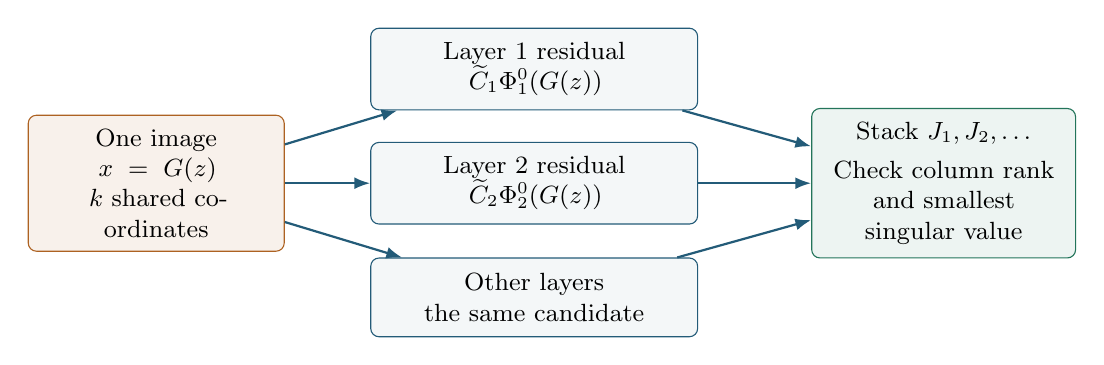
\begin{tikzpicture}
\node[free,text width=2.9cm] (candidate) at (0,-1.45) {One image\\$x=G(z)$\\$k$ shared coordinates};
\node[box,text width=3.8cm] (l1) at (4.8,0) {Layer 1 residual\\$\widetilde C_1\Phi_1^0(G(z))$};
\node[box,text width=3.8cm] (l2) at (4.8,-1.45) {Layer 2 residual\\$\widetilde C_2\Phi_2^0(G(z))$};
\node[box,text width=3.8cm] (l3) at (4.8,-2.9) {Other layers\\the same candidate};
\node[learn,text width=3cm] (stack) at (10,-1.45) {Stack $J_1,J_2,\ldots$\\[3pt] Check column rank\\and smallest singular value};
\draw[arr] (candidate) -- (l1);
\draw[arr] (candidate) -- (l2);
\draw[arr] (candidate) -- (l3);
\draw[arr] (l1) -- (stack);
\draw[arr] (l2) -- (stack);
\draw[arr] (l3) -- (stack);
\end{tikzpicture}
\caption{All layers constrain the same latent change. Adding a block helps only if its rows add useful sensitivity; approximate layers also contribute residual error. Independent per-layer candidates would break this compatibility.}
\label{fig:stackedlayers}
\end{figure}
\FloatBarrier

\begin{definition}[Layerwise visibility]
Fix $L$ adapted layers. At layer $\ell$, let $n_\ell$ be the feature dimension, $\HH_\ell$ the fixed private reference span with dimension $q_\ell$, $r_\ell$ the adapter rank, and
\[
p_\ell=r_\ell-q_\ell,\qquad b_\ell=n_\ell-q_\ell,
\qquad 0\le p_\ell\le b_\ell.
\]
An empty block $p_\ell=0$ contributes no certificate equations. For an image chart $G:\Omega\subset\R^k\to\XX$, put $\phi_\ell=\Phi_\ell^0\circ G$ and, at a fixed $z_*$, choose an orthonormal basis $Q_{1,\ell}$ of $\HH_\ell^\perp$. Define
\[
V_\ell=Q_{1,\ell}^TD\phi_\ell(z_*)\in\R^{b_\ell\times k},\qquad
W_\ell=\row V_\ell\subset\R^k.
\]
$W_\ell$ is the latent cotangent subspace the layer can measure after removing its private span. The ideal random model below uses independent matrices $E_\ell\in\R^{p_\ell\times b_\ell}$ with densities, and stacked Jacobian
\[
J=\begin{bmatrix}E_1V_1\\ \vdots\\ E_LV_L\end{bmatrix}.
\]
Exact Gaussian certificates with independent initializations have this rank model, up to invertible transformations of each row block. The backbone maps, reference spans, chart, and point are fixed before drawing these matrices.
\end{definition}

\subsection{The geometric condition behind a generic full-rank stack}

\proofidea{Each layer can supply only a limited number of rows from its own available subspace. For every collection of layers, compare the dimension available inside that collection with the number of rows supplied outside it. The minimum of these possibilities is the exact generic rank.}

\begin{lemma}[Selecting independent vectors from subspaces]\label{lem:selection}
For subspaces $W_1,\ldots,W_t$ of a finite-dimensional vector space, the maximum rank of a list $w_j\in W_j$ is
\[
\rho=\min_{I\subset\{1,\ldots,t\}}\left(t-|I|+\dim\sum_{j\in I}W_j\right).
\]
\end{lemma}
\begin{proof}
First prove the full-independence assertion: independent representatives exist if
\[
\dim\sum_{j\in I}W_j\ge|I|\quad\text{for every }I.
\]
Use induction on $t$. The case $t=1$ is immediate. If a nonempty proper subset $I$ is tight, meaning its sum has dimension $|I|$, choose independent representatives on $I$ by induction. In the quotient by $U=\sum_{j\in I}W_j$, the remaining spaces satisfy the same condition, because for every remaining subset $K$,
\[
\dim\big((U+\sum_{j\in K}W_j)/U\big)
\ge |I|+|K|-|I|=|K|.
\]
Inductively select independent quotient representatives and lift them; together with those on $I$ they are independent. If there is no proper nonempty tight subset, choose a nonzero representative in $W_t$. In the quotient by its span, every nonempty subset of the remaining spaces loses at most one dimension and originally had dimension at least its size plus one. The induction hypothesis again supplies the other representatives. This proves the assertion.

For general $\rho$, any selection has rank at most the displayed expression for each $I$, because the vectors indexed outside $I$ add at most $t-|I|$ dimensions. For the reverse bound, append to the ambient space a new space $U$ of dimension $t-\rho$ and replace each $W_j$ by $W_j\oplus U$. For every nonempty $I$, its sum has dimension $\dim\sum_{j\in I}W_j+t-\rho\ge|I|$ by the definition of $\rho$. The full-independence assertion gives $t$ independent representatives in this enlarged space. Projecting back to the original space loses at most $t-\rho$ dimensions, so their original components have rank at least $\rho$. Each belongs to the prescribed $W_j$, proving equality.
\end{proof}

\begin{theorem}[Exact generic rank across layers]\label{thm:layerrank}
Under the fixed-object and independent-density assumptions in the preceding definition, almost surely
\begin{equation}\label{eq:layerrank}
\rank J=
\min_{I\subset\{1,\ldots,L\}}\left(
\sum_{\ell\notin I}p_\ell+\dim\sum_{\ell\in I}W_\ell
\right).
\end{equation}
Consequently the ideal stacked chart derivative is injective if and only if
\begin{equation}\label{eq:hall}
\dim\sum_{\ell\in I}W_\ell+\sum_{\ell\notin I}p_\ell\ge k
\quad\text{for every }I\subset\{1,\ldots,L\}.
\end{equation}
The condition $\sum_\ell p_\ell\ge k$ is merely the $I=\varnothing$ member of this family. If every layer has $W_\ell=\R^k$, that total-row condition is sufficient for almost-sure injectivity. It does not give a conditioning floor.
\end{theorem}
\begin{proof}
Each of the $p_\ell$ rows in block $E_\ell V_\ell$ can vary over $W_\ell$. Apply Lemma~\ref{lem:selection} to a list containing $p_\ell$ copies of this subspace. In its minimum, once a subset contains a row from a block, adding all remaining rows of that block cannot increase the expression: the summed subspace is unchanged and the number of omitted rows decreases. Thus the minimum can be taken over whole blocks, giving \eqref{eq:layerrank} as the maximum achievable rank.

There is therefore a deterministic choice of all $E_\ell$ realizing that rank. A corresponding nonzero minor of the stack is a polynomial in their entries which is not identically zero. The joint density of the independent matrices assigns probability zero to its zero set. Conversely, the subspace bound in the lemma applies to every choice of entries. This proves the almost-sure equality. Since all $W_\ell$ lie in $\R^k$, the minimum is at most $k$ by taking all layers. Equality to $k$ is exactly \eqref{eq:hall}. If every nonempty sum is $\R^k$, only the empty-subset constraint remains. Stable local inversion then uses Theorem~\ref{thm:master} and the realized smallest singular value.
\end{proof}

\begin{corollary}[Same-input adapters and shared or independent seeds]\label{cor:sameinput}
Suppose all $L$ adapters see exactly the same $h\in\R^n$ and private span $\HH$ of dimension $q$. Let $P=\sum_\ell(r_\ell-q)$ and $b=n-q$. With independent Gaussian initializations and exact kernels, their stacked certificate has rank $t=\min(P,b)$. On a fixed immersed tangent of dimension $k$ with $d=\dim(T\cap\HH)$, its rank is
\[
\min(P,k-d).
\]
Whitening the complete stacked row space gives a uniform $t$-plane in $\HH^\perp$. The single-certificate beta laws and conditioning bounds apply to it with $p$ replaced by $t$. If $P\ge b$, the common kernel is exactly $\HH$.

If instead every certificate is a row transformation of the same certificate, stacking has exactly its original kernel and rank, no matter how many blocks are released.
\end{corollary}
\begin{proof}
Stack the independent Gaussian quotient matrices; the result is a standard Gaussian $P\times b$ matrix, so its row rank is $\min(P,b)$ almost surely. Its restriction to the fixed projected tangent has rank $\min(P,k-d)$ by the same minor argument. Rotation invariance gives uniformity of the aggregate row space and transfers the laws in Section 2. When its rank is $b$, it measures all of $\HH^\perp$. For repeated row spaces, intersecting the same kernel repeatedly leaves it unchanged. Thus same-input geometry does not by itself make Q/K/V redundant; independence or correlation of their actual sensing subspaces matters.
\end{proof}

\subsection{A stack can be full rank and still be too poorly conditioned}

\begin{theorem}[A quantitative bound for heterogeneous layers]\label{thm:layercond}
Assume the $E_\ell$ in Theorem~\ref{thm:layerrank} are independent standard Gaussian matrices. Define the expected Gram matrix
\[
S_0=\sum_{\ell=1}^L p_\ell V_\ell^TV_\ell,
\]
assume $S_0\succ0$, and define the maximum row covariance after normalization
\[
v_0=\max_{\ell:p_\ell>0}
\norm{S_0^{-1/2}V_\ell^TV_\ell S_0^{-1/2}}.
\]
For $0<t_0<1$, with probability at least
\[
1-2\,9^k\exp\{-t_0^2/(32v_0)\},
\]
\begin{equation}\label{eq:layerbound}
J^TJ\succeq(1-t_0)S_0,
\qquad \smin(J)\ge\sqrt{(1-t_0)\lambda_{\min}(S_0)}.
\end{equation}
Here $\succeq$ denotes the positive-semidefinite ordering. A negative probability lower bound is vacuous, not a full-rank conclusion. In particular $S_0\succ0$ alone is not sufficient for realized rank.
\end{theorem}
\begin{proof}
Put $\widetilde J=JS_0^{-1/2}$. Its independent Gaussian rows have covariance matrices $S_j$ with $\sum_jS_j=I_k$ and $\norm{S_j}\le v_0$. For a unit vector $u$, write $a_j=u^TS_ju$. Then $a_j\ge0$, $\sum_ja_j=1$, $\max_ja_j\le v_0$, and
\[
\norm{\widetilde Ju}^2-1\ \stackrel{d}=\ \sum_j a_j(g_j^2-1)
\]
for independent standard Gaussian $g_j$. For $|\lambda|\le1/(4v_0)$, the Gaussian moment-generating function and the power series for $-\log(1-x)$ give
\[
\log\E\exp\!\left(\lambda\sum_j a_j(g_j^2-1)\right)
\le2\lambda^2\sum_j a_j^2\le2\lambda^2v_0.
\]
Chernoff's inequality with $\lambda=e/(4v_0)$, and then with its negative, yields
$\Prob\{|\norm{\widetilde Ju}^2-1|\ge e\}\le2\exp(-e^2/(8v_0))$ for $0<e\le1$.

A Euclidean $1/4$-net of the unit sphere has at most $9^k$ points; this follows by taking disjoint radius-$1/8$ balls around a maximal separated set and comparing volumes. For any symmetric matrix $M$, approximation of a unit vector maximizing $|u^TMu|$ by the net gives $\norm M\le2\max_{u\text{ in net}}|u^TMu|$, since the difference is at most $2(1/4)\norm M$. Apply the scalar bound with $e=t_0/2$, union-bound the net, and take $M=\widetilde J^T\widetilde J-I_k$. This proves $\norm M\le t_0$ with the stated probability, hence \eqref{eq:layerbound} after conjugation by $S_0^{1/2}$. The bound explicitly includes the concentration requirement; expectation alone never entered as a rank assertion.
\end{proof}

\subsection{Deeper-layer drift: combine the error budgets as well as the rows}

\begin{theorem}[Perturbed certificates and accumulation across layers]\label{thm:layernoise}
Let $\widetilde C_\ell$ be the actual, possibly truncated certificate and $\phi_\ell(z)=\Phi_\ell^0(G(z))$. At a true chart point $z_*$ assume
\[
\norm{\widetilde C_\ell\phi_\ell(z_*)}\le K_\ell\varepsilon.
\]
Choose fixed nonnegative weights $w_\ell$ and define
\[
f_w(z)=(\sqrt{w_\ell}\widetilde C_\ell\phi_\ell(z))_{\ell=1}^L,
\quad J_w=Df_w(z_*),\quad\alpha_w=\smin(J_w)>0,
\quad B_w=\varepsilon\sqrt{\sum_\ell w_\ell K_\ell^2}.
\]
On a closed ball where $\sup\norm{Df_w-J_w}\le\alpha_w/2$, every minimizer of $\norm{f_w}$ satisfies
\begin{equation}\label{eq:multinoisy}
\norm{\widehat z-z_*}\le4B_w/\alpha_w.
\end{equation}
For an off-chart $x_*$, take $x_0=G(z_0)$ with error $\delta$ and assume $\Phi_\ell^0$ is $L_\ell$-Lipschitz between $x_*,x_0$. The same conclusion centered at $z_0$ holds with
\[
B_w=\left[\sum_\ell w_\ell
\big(K_\ell\varepsilon+\norm{\widetilde C_\ell}L_\ell\delta\big)^2\right]^{1/2},
\]
followed by the image error $\delta+4L_GB_w/\alpha_w$.

If an ideal stacked derivative $J^0$ has $\smin(J^0)=\alpha_0$ and $\norm{J_w-J^0}\le e_J<\alpha_0$, then $\alpha_w\ge\alpha_0-e_J$. A bound only on $\widetilde C_\ell h_{\ell,i}^0$ does not imply this derivative perturbation condition. Whitening a rank-$p_\ell$ approximate certificate changes the available residual bound to $K_\ell\varepsilon/\sigma_{p_\ell}(\widetilde C_\ell)$, by applying its inverse nonzero singular values.
\end{theorem}
\begin{proof}
The hypotheses give $\norm{f_w(z_*)}\le B_w$. Optimality implies $\norm{f_w(\widehat z)}\le B_w$, so their difference has norm at most $2B_w$. The segment estimate from Theorem~\ref{thm:master}, centered at $z_*$ but not requiring its residual to be zero, is at least $\alpha_w\norm{\widehat z-z_*}/2$. This proves \eqref{eq:multinoisy}. The off-chart residual bound follows by adding and subtracting $\widetilde C_\ell\Phi_\ell^0(x_*)$, applying each Lipschitz estimate, and summing weighted squares. The feature-to-image estimate is the triangle inequality as in Theorem~\ref{thm:robust}. Finally, for every unit $v$, $\norm{J_wv}\ge\norm{J^0v}-\norm{(J_w-J^0)v}\ge\alpha_0-e_J$. Values of an operator on finitely many training vectors do not bound it on chart tangents, which proves the last limitation, also illustrated in Section 5.
\end{proof}

\begin{proposition}[When an additional noisy layer hurts]\label{prop:hurt}
For an affine local residual $f_\ell(z_*+v)=b_\ell+J_\ell v$, the unique weighted least-squares displacement, when $S_w=\sum_\ell w_\ell J_\ell^TJ_\ell\succ0$, is
\[
\widehat v=-S_w^{-1}\sum_\ell w_\ell J_\ell^Tb_\ell.
\]
Adding rows can increase $S_w$ and improve its smallest eigenvalue while increasing deterministic reconstruction error. If instead $b_\ell$ are independent, zero-mean random errors, independent of fixed $J_\ell$, with covariance $\sigma_\ell^2I$ and $w_\ell=\sigma_\ell^{-2}$, then
\[
\operatorname{Cov}(\widehat v)=S_w^{-1}.
\]
Under those additional stochastic assumptions adding a layer cannot increase this covariance in positive-semidefinite order.
\end{proposition}
\begin{proof}
Differentiating the quadratic loss gives the normal equation $S_w\widehat v=-\sum_\ell w_\ell J_\ell^Tb_\ell$. With scalar $z$, take one residual $z$ and add $z-\varepsilon$: the exact solution moves from $0$ to $\varepsilon/2$ while $S_w$ grows from $1$ to $2$. For the stochastic case, independence removes cross covariances and $w_\ell^2\sigma_\ell^2=w_\ell$, yielding $S_w^{-1}S_wS_w^{-1}=S_w^{-1}$. If $S_{\rm new}=S_w+T$ with $T\succeq0$, conjugating by $S_w^{-1/2}$ shows $(I+S_w^{-1/2}TS_w^{-1/2})^{-1}\preceq I$, hence $S_{\rm new}^{-1}\preceq S_w^{-1}$. Deterministic certificate drift has no asserted zero mean, so this covariance argument cannot be assumed for it.
\end{proof}

\subsection{Where the chart lives determines whether the constraints agree}

\begin{theorem}[Compatible locations for a multilayer chart]\label{thm:compatibility}
An image chart $G(z)$ defines mutually compatible layer charts $\phi_\ell(z)=\Phi_\ell^0(G(z))$. A chart $u=\psi_1(z)$ at a first adapted layer is equivalent for all feature residuals if, on the candidate set, every relevant layer feature factors through it:
\[
\Phi_\ell^0(x)=T_\ell(\Phi_1^0(x)),
\]
for known maps $T_\ell$, and $\psi_1$ has an image-side realization when image recovery is required. This factorization is a sufficient-state assumption, which may fail if another branch carries unrepresented information.

Alternatively, introduce per-layer variables $u_\ell\in\R^{n_\ell}$ and enforce the consistency equations
\[
u_\ell-\phi_\ell(z)=0,\qquad \widetilde C_\ell u_\ell=0.
\]
Their feasible set is exactly the common-chart zero set lifted to the graph $u_\ell=\phi_\ell(z)$. Their derivative is injective exactly when the common-chart stacked derivative is injective. Independent per-layer charts without these consistency equations need not correspond to any common input.
\end{theorem}
\begin{proof}
The image-side construction is composition of known maps, so all features come from the same image. Under the factorization, replacing each $\phi_\ell$ by $T_\ell\circ\psi_1$ gives the same feature residuals pointwise. The realization condition is Theorem~\ref{thm:feature}; an inverse bound is additionally needed for stable image readout. For the graph formulation, the first equations uniquely determine every $u_\ell$ from $z$, proving equality of feasible sets after elimination. A tangent in the joint derivative kernel obeys $\dot u_\ell=D\phi_\ell(z_*)\dot z$ and $\widetilde C_\ell\dot u_\ell=0$. Eliminating the $\dot u_\ell$ yields precisely the stacked chart kernel. Conversely every vector in that kernel lifts to one in the graph kernel. Removing consistency removes this equivalence and permits independent feature choices.
\end{proof}

\begin{remark}[The exact reading of ``200 equations'']
Let $a_{\rm raw}$ denote the number of scalar residual coordinates over a complete training tuple. It is a bookkeeping bound on derivative rank. With independent per-image latent dimension $k$ the tuple dimension is $Mk$; with a shared concept it is $s+\sum_i t_i$. The relevant necessary condition for a Lipschitz-stable inverse is $a_{\rm raw}$ at least this actual latent dimension after nuisance elimination, and the operative sufficient condition is a positive smallest singular value of the corresponding derivative. For a certificate, $q_\ell$ determines each available row space; it is not interchangeable with $M$. Theorem~\ref{thm:layerrank} supplies the missing geometric condition for an ideal independent-layer model. For actual drifting layers one must additionally control the actual derivative as in Theorem~\ref{thm:layernoise}. A singular-value gap in $B_{\ell,T}$ protects the certificate's construction; it is not the chart's inverse-conditioning constant.
\end{remark}

\clearpage
\section{Research ideas, ranked by promise}\label{sec:ideas}

\chapterbrief
{The most promising starting point is a fixed subject-relevant public chart with checked coverage and sensitivity. Shared concepts, complementary layers, and certificate-guided replay can then address specific remaining ambiguities. These are research directions with proved mechanisms, not established performance claims for natural images.}
{Each proposal follows the same four questions: what would we claim, what mathematics supports the mechanism, what assumption remains unproved, and what would make us abandon it? The ranking is a reasoned research judgment, not an experimental comparison.}
{$\delta$ denotes missing chart coverage; $k$ counts searched coordinates; $p=r-q$ is exact certificate rank. A proposal succeeds through the actual restricted Jacobian and exclusions of aliases, never through $p$ alone.}

The ordering weighs a mathematically defensible claim and usefulness in the stated released-adapter setting. Each item distinguishes its proved mechanism from the unproved claim needed for real features.

\begin{proposal}[1. A fixed subject-conditioned chart, with a recovery criterion]
\textbf{Claim to pursue.} Use a fixed generator $G_c(z)$ or feature chart $\psi_c(z)$ for a declared condition $c$, and establish small representation error and a lower bound on the restricted observation derivative. For a certificate-only claim, also establish $\im\psi_c\cap\HH$ contains only the intended private representations.

\textbf{Proved mechanism.} Theorems~\ref{thm:robust}, \ref{prop:sectional}, and \ref{thm:global} convert those properties into local stability and, with $k<p$, global absence of random-kernel aliases. A fixed text-conditioned generator is a legitimate chart; varying its text or weights adds parameters that must be included in its derivative. A feature autoencoder is legitimate only with its actual feature coverage and readout properties stated.

\textbf{Open obstacle.} A semantic label such as ``golden retriever'' gives neither instance-level coverage nor span separation. A generator can omit the particular dog, pose, or background. \textbf{Kill criterion.} A lower bound on unavoidable $\delta$ already exceeds the desired reconstruction accuracy, or every relevant tangent has a certificate-invisible direction. A high-fidelity rendering is not a substitute for either condition.
\end{proposal}

\begin{proposal}[2. Recover the shared concept before the individual nuisances]
\textbf{Claim to pursue.} In $x_i=G(z,u_i)$, identify $z$ through the projected shared Jacobian $K_s$, and recover the full tuple when each nuisance derivative is injective. Public conditioning may reduce the shared dimension without fixing the instance in advance.

\textbf{Proved mechanism.} Theorem~\ref{thm:shared} gives an exact rank criterion and a conditioning bound. Diverse per-example nuisance tangent spaces can make the stacked projected shared derivative injective even when one example does not determine the shared concept.

\textbf{Open obstacle.} The shared/nuisance split can have a gauge: a change in $z$ may be absorbed by every $u_i$. The chart can also generate repeated images. \textbf{Kill criterion.} $K_s$ is singular after legitimate gauge fixing, or all proposed diversity constraints still allow a collapsed tuple. Repetition of the same shared sensitivity does not guarantee new rank.
\end{proposal}

\begin{proposal}[3. Solve replay on the certificate fiber]
\textbf{Claim to pursue.} If the certificate residual has constant rank $s$ on a $k$-dimensional chart, locally parameterize its zero fiber and optimize replay using only $k-s$ data coordinates, plus its honest seed and recipe nuisance variables.

\textbf{Proved mechanism.} Theorem~\ref{thm:compose} gives the exact reduction and the test $\rank(J_R|_{\ker J_C})=k-s$. Theorem~\ref{thm:nuisance} says how to test this after allowing unknown continuous seed and recipe directions. This is a potential computational advantage; it does not add information to an exact replay problem that already implies the certificate.

\textbf{Open obstacle.} Parameterizing the relevant fiber and finding its correct connected component may be hard. Approximate deeper certificates do not define a zero fiber through the truth. \textbf{Kill criterion.} Replay vanishes on a nontrivial tangent of that fiber after nuisance projection, or the fiber cannot be represented more cheaply than the original chart. A local rank theorem does not prove a global speedup.
\end{proposal}

\begin{proposal}[4. Select the concept with an overdetermined residual, then invert it]
\textbf{Claim to pursue.} Fix a finite family of public sectional charts before seeing the initialization. Use residuals to reject incompatible concepts, then search the remaining charts.

\textbf{Proved mechanism.} Theorem~\ref{thm:wrong} and Corollary~\ref{cor:test} give an exact affine test when the wrong charts stay a positive distance from $\HH$ and $p>k$. Theorem~\ref{thm:entropy} treats fixed compact nonlinear charts and makes their size part of the false-positive bound. A whitened residual is preferable to an unqualified $\lambda_1$ test because it avoids a zero eigenvalue attained only at infinity.

\textbf{Open obstacle.} The distance from a wrong semantic concept to the private span is unknown. More flexible concepts overfit more easily; a search over many adaptive charts invalidates a single-chart tail. \textbf{Kill criterion.} Candidate concepts share a certified span point, the affine test is saturated at $p=k$, or no useful positive separation assumption can be justified. Low residual identifies compatibility, not semantic truth by definition.
\end{proposal}

\begin{proposal}[5. Use span-separating expansion families as a theory target]
\textbf{Claim to pursue.} Analyze an adapted network whose input features have the polynomial or quadratic structure of Theorems~\ref{thm:polynomial} and \ref{thm:quadratic}. This yields a complete theorem about individual-point recovery from the certificate, rather than leaving ``a good manifold'' as an unexplained assumption.

\textbf{Proved mechanism.} The polynomial argument separates every extra candidate by a polynomial vanishing on the private set; the quadratic argument uses rank-one matrices and affine independence. Both prove tangent disjointness as well as global span separation.

\textbf{Open obstacle.} Real frozen features need not approximate these representations in a norm strong enough to preserve separation and conditioning. \textbf{Kill criterion.} The claim requires adding features that the adapted layer never observed, or the embedding is so poorly conditioned that the resulting stability bound is unusable. This is a constructive architectural theorem, not permission to claim generic natural-image separation.
\end{proposal}

\begin{proposal}[6. Choose layers by complementary sensitivities and error]
\textbf{Claim to pursue.} On one common image chart, prefer layer sets whose chart Jacobians have a well-conditioned joint span while their certificate residual bounds remain small. Independent same-input adapters can be useful; deeper layers can be useful if they contribute new tangent sensitivity.

\textbf{Proved mechanism.} Theorem~\ref{thm:layerrank} characterizes generic rank, Theorem~\ref{thm:layercond} provides a quantitative sufficient condition, and Theorem~\ref{thm:layernoise} supplies the competing noise cost. Under a justified stochastic noise model, inverse-variance weighting has Proposition~\ref{prop:hurt}'s covariance guarantee.

\textbf{Open obstacle.} Deterministic drift and initialization-dependent selection need not fit that stochastic model. \textbf{Kill criterion.} New rows lie in the existing row space, or their increase in bias dominates the gain in conditioning. ``More layers'' is not the criterion.
\end{proposal}

\begin{proposal}[7. Finite-candidate testing as a sharper, smaller objective]
\textbf{Claim to pursue.} When a meaningful public candidate list exists, test it directly rather than generate an entire image manifold.

\textbf{Proved mechanism.} Theorem~\ref{thm:membership} gives exact rejection of fixed candidates outside $\HH$ and a normalized null law under a separation assumption. Searching a finite list avoids an optimization problem and requires no latent dimension bound. This can be an identification theorem if the list contains the true points and no nonmember lies in their span.

\textbf{Open obstacle.} Near-duplicate candidates may lie close to the private span, and public lists can miss the instance. \textbf{Kill criterion.} Two semantically different candidates lie in the same certified span, or the intended output requires distinguishing multiplicity or exact training membership without the needed candidate-set assumption. The valid generic statement is span membership, not unconditional training membership.
\end{proposal}

\begin{proposal}[8. Additional information in the endpoint, with nuisance elimination]
\textbf{Claim to pursue.} Seek a released-only nonlinear residual involving the noncertificate part of $A_T$ and $B_T$ whose derivative is injective on some remaining certificate directions after profiling out unknown seed and recipe.

\textbf{Proved mechanism available now.} The composition and nuisance theorems give the correct acceptance test for such a residual. The identity $\mathbf1^TB_T=0$ at a softmax classifier head is not itself an instance-resolving constraint: with cross-entropy every per-example logit gradient sums to zero, hence every scalar combination of their updates preserves that equality for every dataset. It only restricts the admissible output subspace and caps $\rank B_T\le m-1$ in that setting.

\textbf{Open obstacle.} Trajectory coefficients and quantitative singular values may contain extra information, but their dependence on data, seed, and recipe must be modeled. They are not public per-example coefficients merely because $B_T$ is public. \textbf{Kill criterion.} The proposed residual is data-independent, a function of the already imposed residuals at regular points, or has zero derivative on the unresolved chart tangent after nuisance elimination. No universal extra independent-row claim is proved here.
\end{proposal}

\clearpage
\section{Small explicit counterexamples}\label{sec:counterexamples}

\chapterbrief
{Several tempting shortcuts fail even in tiny dimensions: a perfect score can belong to the wrong chart, an isolated solution can be unstable, duplicate layer rows add no rank, and better conditioning can coexist with worse biased recovery. These examples explain why the assumptions in the earlier chapters are needed.}
{Choose an example by the claim it challenges, then inspect its matrices and residual. The examples distinguish algebraic certificate realizations from actual training trajectories; only the explicitly constructed trajectories make training-dynamics claims.}
{$A$ abbreviates $A_T$; $n,r,q,k,L$ are feature dimension, adapter rank, private span rank, chart dimension, and number of layers. The standard basis vector $e_i$ has one in coordinate $i$ and zeros elsewhere.}

In the following displays, $A$ means $A_T$. Whenever $A_0=A$ is written, it specifies an algebraic realization of the supplied kernel identities, not a claim that this particular matrix has positive probability under a continuous law. The optimizer counterexample separately verifies a positive-probability failure. Set $s=1$ and $W_0=0$ wherever a training run is specified.

\begin{center}
\small
\begin{tabular}{@{}Y{.40\textwidth}Y{.50\textwidth}@{}}
\toprule
Tempting inference & Where it fails\\\\
\midrule
Zero score means the right image & Counterexamples~\ref{ex:wrongzero}, \ref{ex:remote}, \ref{ex:nonlinear}: wrong charts, remote aliases, and span mixtures\\\\[4pt]
Isolation means a stable inverse & Counterexample~\ref{ex:singular}: zero derivative and square-root sensitivity\\\\[4pt]
More layers necessarily help & Counterexamples~\ref{ex:redundant}, \ref{ex:noisy}, \ref{ex:pointwise}: redundancy, bias, and invisible tangents\\\\[4pt]
Certified features determine pixels & Counterexample~\ref{ex:preimage}: absent or nonunique image preimages\\\\
\bottomrule
\end{tabular}
\end{center}

\begin{example}[Scalar decay can erase the certificate]\label{ex:decay}
Take $n=r=2$, $m=1$, $q=1$, $k=1$, $L=1$, $h_*=e_1=(1,0)^T$, $A_0=I_2$, $B_0=(0,0)$, and loss $\frac12(BAh_*-1)^2$. One SGD step of size $1/2$ without decay gives
\[
A_1=\begin{bmatrix}1&0\\0&1\end{bmatrix},\qquad B_1=\begin{bmatrix}1/2&0\end{bmatrix}.
\]
The prediction is $1/2$, hence its loss derivative is $-1/2$. A second simultaneous gradient step of size one with scalar weight decay one gives
\[
A_2=(1-1)A_1-\nabla_A\ell
=\begin{bmatrix}1/4&0\\0&0\end{bmatrix},\qquad
B_2=(1-1)B_1-\nabla_B\ell=\begin{bmatrix}1/2&0\end{bmatrix}.
\]
Thus $\rank B_2=q=1$ but $C=P_{\row B_2^\perp}A_2=0$. The chart $(1,w)^T$ may be used, but no certificate direction survives. For any seed near $I_2$, put $v=A_0e_1$ and $\rho=\frac12\norm v^2-1$. The same calculation gives $A_2=-\frac12\rho v e_1^T$ and $B_2=-\rho v^T$. For $v\ne0$ and $\rho\ne0$, which holds on an open neighborhood of $I_2$, $B_2$ has rank one and $C=0$. A density supported in that neighborhood gives a probability-one counterexample to the unrestricted optimizer formulation.
\end{example}

\begin{example}[The smallest eigenvalue lives at infinity]\label{ex:infinity}
Take $n=r=2$, $q=k=L=1$,
\[
H=\begin{bmatrix}1\\0\end{bmatrix},\quad A_0=A=I_2,\quad
B=\begin{bmatrix}1&0\end{bmatrix},\quad
C=\begin{bmatrix}0&0\\0&1\end{bmatrix},\quad
\mu=\begin{bmatrix}0\\1\end{bmatrix},\quad U=\begin{bmatrix}1\\0\end{bmatrix}.
\]
Then $\psi(w)=(w,1)^T$, $\mathcal G=\begin{bmatrix}0&1\\1&0\end{bmatrix}$ is invertible, and $R(\psi(w))=1/(1+w^2)$. The smallest pencil eigenvalue is zero with eigenvector $(0,1)^T$, but there is no finite zero or finite minimizer.
\end{example}

\begin{example}[A full-rank wrong chart has a perfect zero]\label{ex:wrongzero}
Take $n=3$, $r=2$, $q=k=L=1$ and
\[
H=\begin{bmatrix}1\\0\\0\end{bmatrix},\quad
A_0=A=\begin{bmatrix}1&0&0\\0&1&0\end{bmatrix},\quad
B=\begin{bmatrix}1&0\end{bmatrix},\quad
C=\begin{bmatrix}0&0&0\\0&1&0\end{bmatrix}.
\]
The affine chart $\psi(w)=(1,w,1)^T$ never meets $\HH=\operatorname{span}(e_1)$, but $CU=(0,1)^T$ has full column rank and its unique zero is $(1,0,1)^T$. Its score is $w^2/(1+w^2)$. This is the saturated case $p=k$, with an alias in the initialization kernel direction $e_3$.
\end{example}

\begin{example}[Zero chart error and perfect local rank do not locate the global minimizer]\label{ex:remote}
Keep every matrix and dimension in Counterexample~\ref{ex:wrongzero}. For any $D_0>0$ let
\[
\psi(w)=(1,w(w-1),D_0w)^T.
\]
The true point is $\psi(0)=e_1$, so representation error is zero. The certificate derivative there has norm one. Nevertheless $\psi(1)=(1,0,D_0)^T$ is another global zero at distance $D_0$. Thus local conditioning and $\delta$ alone cannot bound an unrestricted minimizer's error.
\end{example}

\begin{example}[Isolation does not require a full-rank derivative]\label{ex:singular}
For a one-dimensional example use the matrices in Counterexample~\ref{ex:infinity} and $\psi(w)=(1,w^2)^T$. Its only zero is $w=0$, but the residual derivative vanishes and $R=w^4/(1+w^4)$. A residual perturbation from $w^2$ to $w^2-\varepsilon$ moves roots by $\sqrt\varepsilon$, not $O(\varepsilon)$.

For an immersed chart showing that pointwise rank does not imply a fiber dimension, use $n=4$, $r=3$, $q=1$, $k=2$, $L=1$:
\[
A_0=A=\begin{bmatrix}1&0&0&0\\0&1&0&0\\0&0&0&1\end{bmatrix},\quad
B=\begin{bmatrix}1&0&0\end{bmatrix},\quad H=e_1,
\quad C=\begin{bmatrix}0&0&0&0\\0&1&0&0\\0&0&0&1\end{bmatrix}.
\]
The chart $\psi(u,v)=(1,u,v,v^2)^T$ is immersed everywhere. Its residual is $(0,u,v^2)^T$, which has derivative rank one at $(0,0)$ but an isolated zero. There is no one-dimensional zero fiber there.
\end{example}

\begin{figure}[htbp]
\centering
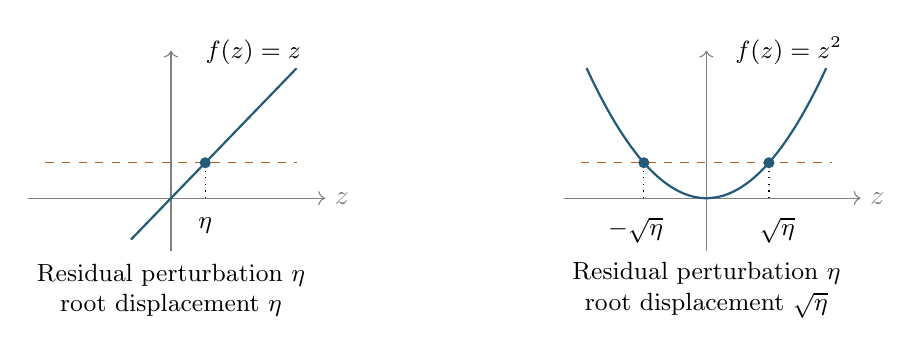
\begin{tikzpicture}[x=1.45cm,y=1.5cm]
\begin{scope}
\draw[->,gray] (-1.25,0) -- (1.35,0) node[right] {$z$};
\draw[->,gray] (0,-.45) -- (0,1.25);
\draw[thick,chartblue,domain=-.35:1.1] plot (\x,\x);
\draw[dashed,chartorange] (-1.1,.30) -- (1.1,.30);
\draw[dotted] (.30,0) -- (.30,.30);
\fill[chartblue] (.30,.30) circle (2pt);
\node[font=\small,above] at (.72,1.05) {$f(z)=z$};
\node[font=\small,below] at (.30,-.08) {$\eta$};
\node[font=\small,align=center] at (0,-.78) {Residual perturbation $\eta$\\root displacement $\eta$};
\end{scope}
\begin{scope}[xshift=6.8cm]
\draw[->,gray] (-1.25,0) -- (1.35,0) node[right] {$z$};
\draw[->,gray] (0,-.45) -- (0,1.25);
\draw[thick,chartblue,domain=-1.05:1.05,samples=50] plot (\x,{\x*\x});
\draw[dashed,chartorange] (-1.1,.30) -- (1.1,.30);
\draw[dotted] (.5477,0) -- (.5477,.30);
\draw[dotted] (-.5477,0) -- (-.5477,.30);
\fill[chartblue] (.5477,.30) circle (2pt);
\fill[chartblue] (-.5477,.30) circle (2pt);
\node[font=\small,above] at (.72,1.05) {$f(z)=z^2$};
\node[font=\small,below] at (.62,-.08) {$\sqrt{\eta}$};
\node[font=\small,below] at (-.62,-.08) {$-\sqrt{\eta}$};
\node[font=\small,align=center] at (0,-.78) {Residual perturbation $\eta$\\root displacement $\sqrt{\eta}$};
\end{scope}
\end{tikzpicture}
\caption{Exact scalar functions illustrating stability, not measured results. Solving $f(z)=\eta$ moves a regular root linearly; the singular isolated root of $z^2$ moves by a square root for $\eta>0$. The second behavior is the failure in Counterexample~\ref{ex:singular}.}
\label{fig:rootstability}
\end{figure}
\FloatBarrier

\begin{example}[Nonlinearity need not separate mixtures]\label{ex:nonlinear}
Take $n=r=3$, $q=2$, $k=L=1$,
\[
H=\begin{bmatrix}1&0\\0&1\\0&0\end{bmatrix},\quad A_0=A=I_3,\quad
B=\begin{bmatrix}1&0&0\\0&1&0\end{bmatrix},\quad
C=\begin{bmatrix}0&0&0\\0&0&0\\0&0&1\end{bmatrix}.
\]
The nonlinear immersed chart $\psi(t)=(\cos t,\sin t,0)^T$ lies wholly in $\HH$. Every point scores zero, including infinitely many nontraining points.

More generally, on any convex region where a feature chart is affine, two distinct certified feature points imply that their entire interpolating segment is certified and remains on that chart region. This follows by linearity of both the chart restriction and $C$. A fixed ReLU expansion composed with a fixed ReLU backbone is piecewise affine, with convex regions for fixed activation patterns. Two private latent points in the same such region therefore cannot be separated by the certificate alone. Merely inserting a ReLU does not prove separation.
\end{example}

\begin{example}[Dimensions do not bound the number of isolated zeros]\label{ex:many}
Use exactly the matrices of Counterexample~\ref{ex:wrongzero}, with $n=3$, $r=2$, $q=k=L=1$. For distinct numbers $a_1=0,a_2,\ldots,a_j$, define
\[
P(t)=\prod_{i=1}^j(t-a_i),\qquad \psi(t)=(1,P(t),t)^T.
\]
This is an injective immersed chart. Its certified representations are exactly the $j$ distinct points $(1,0,a_i)^T$, all with nonzero residual derivative. The true span can remain $\operatorname{span}(e_1)$. The integer $j$ is arbitrary while $n,r,q,k,L$ remain fixed. Taking $\psi(t)=(1,\sin t,t)^T$ gives countably infinitely many isolated zeros on a noncompact chart.
\end{example}

\begin{example}[The normalized score has no kernel-only null law]\label{ex:Rlaw}
Take $n=r=2$, $q=k=L=1$, $H=e_1$, $A_0=I_2$, and for $a\ge1$ set
\[
A_a=\begin{bmatrix}a&0\\0&1\end{bmatrix},\qquad
B_a=\begin{bmatrix}2a-3/2&0\end{bmatrix},\qquad
C_a=\begin{bmatrix}0&0\\0&1\end{bmatrix}.
\]
The kernel and raw certificate are unchanged, yet for the fixed wrong candidate $h=(1,1)^T$,
\[
R_a(h)=1/(a^2+1).
\]
The candidate stays a fixed distance from $\HH$, while its score can be arbitrarily small. These endpoints arise from the scalar squared-loss problem in Counterexample~\ref{ex:decay}: take the same first step, then a second step of size $4(a-1)$ without decay. For a Gaussian seed, write $v=A_0e_1$, $w=A_0e_2$, and $\rho=\|v\|^2/2-1$. A second step of size $t$ gives
\[
A_Th=w+(1-t\rho/2)v,\qquad
Ch=P_{v^\perp}w,\qquad B_T=(1/2-t\rho)v^T.
\]
For each fixed $t$, the exceptional rank failures have probability zero. As $t\to\infty$, $R(h)\to0$ almost surely, whereas before that second step its residual is positive almost surely. Thus even within Gaussian initialization and legitimate SGD, the score law depends on the unspecified training procedure.
\end{example}

\begin{example}[Two layers, two rows, only one identified direction]\label{ex:redundant}
Use $L=2$, $n_1=n_2=3$, $r_1=r_2=2$, $q_1=q_2=1$, and $k=2$. For both layers choose all matrices from Counterexample~\ref{ex:wrongzero}, and use the shared chart $G(z_1,z_2)=(1,z_1,z_2)^T$ with identity feature maps. Compact residuals are both $z_1$, so
\[
J=\begin{bmatrix}1&0\\1&0\end{bmatrix},\qquad \rank J=1<2=p_1+p_2.
\]
Here the sensing rows are correlated. Even independent initializations cannot help if instead both feature maps on the chart equal $(1,z_1,0)^T$: then both $W_\ell=\operatorname{span}((1,0))$, and $z_2$ is structurally invisible for every sensing draw.
\end{example}

\begin{example}[A deeper approximate certificate can worsen recovery]\label{ex:noisy}
Let $L=2$, $n_1=n_2=r_1=r_2=2$, $q_1=q_2=k=1$, $H_1=H_2=e_1$, $B_1=B_2=(1,0)$, and $\phi_1(z)=\phi_2(z)=(1,z)^T$. Let
\[
A_1=\begin{bmatrix}1&0\\0&1\end{bmatrix},\quad
A_2=\begin{bmatrix}1&0\\-\varepsilon&1\end{bmatrix},\quad
C_1=\begin{bmatrix}0&0\\0&1\end{bmatrix},\quad
\widetilde C_2=\begin{bmatrix}0&0\\-\varepsilon&1\end{bmatrix}.
\]
The first residual is $z$ and the second is $z-\varepsilon$. At the truth $z_*=0$, the second error is $\varepsilon$ while $B_2$ has singular value one, so there is no small-gap issue in this example. Equal-weight least squares moves the estimate from zero to $\varepsilon/2$, even though the compact stacked Jacobian's singular value increases from $1$ to $\sqrt2$. This is an operator-level counterexample under the stated approximate-residual assumptions; no claim that this particular pair arose from a specified coupled training run is needed.
\end{example}

\begin{example}[Small residuals do not bound tangent perturbations]\label{ex:pointwise}
Take $n=3$, $r=2$, $q=k=L=1$, $H=e_1$, $B=(1,0)$, and $\psi(z)=(1,z,0)^T$. Compare
\[
A^{(1)}=\begin{bmatrix}1&0&0\\0&1&0\end{bmatrix},\quad
A^{(2)}=\begin{bmatrix}1&0&0\\0&0&1\end{bmatrix},\qquad
C^{(j)}=P_{\row B^\perp}A^{(j)}.
\]
Both rank-one certificates annihilate the true point exactly. But $C^{(1)}\psi$ has derivative $(0,1)^T$, whereas $C^{(2)}\psi$ is identically zero. An error bound only at the training point cannot transfer a tangent-rank theorem from the first operator to the second.
\end{example}

\begin{example}[A certified feature may have no image preimage]\label{ex:preimage}
Let the pixel variable be $x\in\R$, $\Phi(x)=(x,x^2)^T$, and the true image be $x_*=1$. Take $n=r=2$, $q=k=L=1$,
\[
H=\begin{bmatrix}1\\1\end{bmatrix},\quad A_0=A=I_2,\quad
B=\begin{bmatrix}1&1\end{bmatrix},\quad C=\tfrac12\begin{bmatrix}1&-1\\-1&1\end{bmatrix}.
\]
The feature chart $\psi(w)=(w,-1)^T$ has a unique certified point at $w=-1$, namely $(-1,-1)^T\in\HH$. It has no pixel preimage because $x^2$ cannot be $-1$. No decoder can make it an exact realization.

Using instead $\Phi(x)=(1,x^2)^T$ with the same matrices, the two images $x=1$ and $x=-1$ have identical true features. An exact feature inverse cannot determine which image was used.
\end{example}

\clearpage
\section{What remains out of reach}\label{sec:limits}

\chapterbrief
{A chart is a prior restriction, not another measurement. If two admissible inputs yield the same observation, no reconstruction rule can reliably choose between them using that observation alone. This barrier includes span ambiguity, missing image detail, unknown recipes, and the gap between local stability and global search.}
{Read the first proof as the common reason behind the later limits. Each subsequent item identifies a different way two plausible explanations may survive. A justified additional observation or prior exclusion is needed to remove one.}
{$\mathcal O$ is the observation map, $x_1,x_2$ are competing inputs, and $\eta$ is an allowed observation error. The relevant ambiguity is the fiber of $\mathcal O$, not the visual quality of a chosen output.}

\begin{limitation}[An observation fiber is a genuine information barrier]\label{lim:fiber}
Let $\mathcal O$ be any observation map, including its allowed nuisance choices. If two admissible inputs $x_1,x_2$ produce the same observed object, any reconstruction rule based only on that observation has worst-case error at least $\norm{x_1-x_2}/2$ on that pair. This also holds for expected error of a randomized rule. With adversarial observation error at most $\eta$, the same conclusion holds whenever $\norm{\mathcal O(x_1)-\mathcal O(x_2)}\le2\eta$.
\end{limitation}
\begin{proof}
At a common observation the rule has the same output, or output distribution, in both worlds. For every output $\widehat x$, the triangle inequality gives $\norm{\widehat x-x_1}+\norm{\widehat x-x_2}\ge\norm{x_1-x_2}$. Take expectations if needed; one error is at least half the separation. In the noisy case the midpoint of the two observations lies in both admissible noise balls and provides a common observation. A chart helps only by excluding at least one of the two candidate worlds on justified prior grounds.
\end{proof}

\begin{figure}[htbp]
\centering
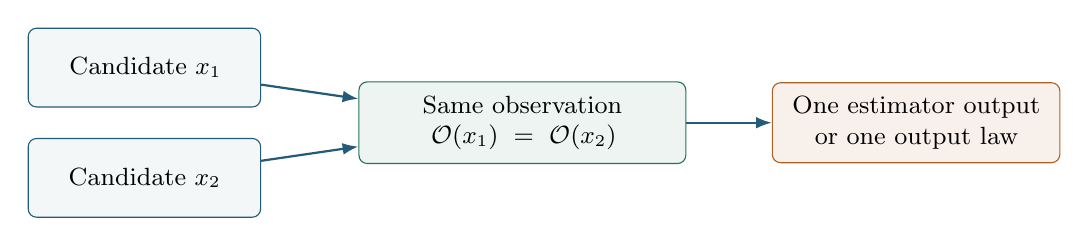
\begin{tikzpicture}
\node[box,text width=2.6cm] (x1) at (0,0) {Candidate $x_1$};
\node[box,text width=2.6cm] (x2) at (0,-1.4) {Candidate $x_2$};
\node[learn,text width=3.8cm] (obs) at (4.8,-.7) {Same observation\\$\mathcal O(x_1)=\mathcal O(x_2)$};
\node[free,text width=3.3cm] (out) at (9.8,-.7) {One estimator output\\or one output law};
\draw[arr] (x1) -- (obs);
\draw[arr] (x2) -- (obs);
\draw[arr] (obs) -- (out);
\end{tikzpicture}
\caption{The information barrier behind the limits. If both candidates remain admissible, at least one expected reconstruction error is at least $\norm{x_1-x_2}/2$. A better decoder cannot remove this ambiguity without an additional observation or justified prior exclusion.}
\label{fig:observationfiber}
\end{figure}
\FloatBarrier

\begin{limitation}[A certificate zero set cannot label its span points]
If two candidate representations both lie in $\HH$, every certificate residual in the same-input setting is zero at both. A chart can isolate the training points only if it excludes the other span points, as the polynomial constructions explicitly do, or if an additional objective distinguishes them. In the normalized Gaussian kernel experiment, the law of the whitened certificate depends on the data only through $\HH$. Thus two different datasets with the same span give the same law in that experiment. This does not claim that the full released pair $(A_T,B_T)$, its scale, or its noncertificate part has no further information.
\end{limitation}

\begin{limitation}[No reconstruction of missing detail from a noninjective feature]
If all chosen residuals factor through a feature map that identifies two chart images, those residuals cannot distinguish the images. A decoder may select a plausible member of that fiber, but exact private-pixel recovery requires an additional injectivity or observation assumption. A feature chart outside the backbone's range creates infeasible solutions, not new recovered images.
\end{limitation}

\begin{limitation}[No global optimizer theorem from local rank]
A positive smallest singular value controls a neighborhood. It does not identify which component contains the truth, prevent distant zeros, guarantee a favorable basin, or establish that a numerical procedure finds every isolated solution. Compactness plus isolation gives finiteness, not a useful bound on the number or an efficient enumeration algorithm. The explicit counterexamples separate all of these issues.
\end{limitation}

\begin{limitation}[No free dimension reduction from the word ``generator'']
A fixed low-dimensional generator can reduce the candidate set. If its weights, conditioning vector, per-image noise, augmentation, or shared code are optimized, their independent parameters belong in the chart and nuisance derivatives. Optimizing a large expansion network is not a $k$-dimensional search just because its fixed input noise has dimension $k$. Conversely, lower latent dimension can destroy coverage of the true image.
\end{limitation}

\begin{limitation}[No universal theorem for the unobserved recipe]
An exact replay residual needs an actual forward training model; an unknown seed or recipe must be searched or eliminated with a justified model. A KKT residual needs its stationarity assumptions. Different discrete recipes can define distinct exact solution branches. None of the chart theorems supplies these missing observations, validates a stationarity identity at arbitrary finite training time, or establishes the proposed capacity line.
\end{limitation}

\begin{limitation}[No unqualified genericity after adaptation]
The random-matrix results hold for fixed public charts and fixed reference spans, or for the explicitly proved uniform statements on such a chart. A chart chosen to fit the released kernel can manufacture zeros. Truncation under input drift produces operators that may depend on all initializations. Their residual bounds and gaps do not, by themselves, imply the independent Gaussian layer model. A successful rigorous extension needs either a derivative perturbation estimate around that model or a direct conditioning theorem for the actual stack.
\end{limitation}

\clearpage
\section{From the theory to an actual expansion network}\label{sec:build}

\chapterbrief
{Freeze a publicly trained decoder and search a small local latent slice. The decoder supplies image structure; the release decides which coordinates are supported. Feature-side search can be cheaper, but a separately trained image readout must be checked against the actual frozen backbone.}
{The first construction is image-side and automatically produces an image. The second searches feature space and adds a readout-and-reencode check. The final result explains why sharper decoding does not create missing evidence.}
{$D_x$ is the frozen image decoder; $a_j,U_j$ define a local latent slice; $z$ or $w$ are searched coordinates. $\Phi^0$ is the actual frozen feature map, not a substitute perceptual encoder.}

This part answers the engineering question that the proofs deliberately leave open: what public map should supply the plausible candidates? The strongest starting point is not a new high-resolution generator trained separately for every adapter. It is a reusable public decoder plus a collection of small coordinate neighborhoods. The following constructions are proposals, not guarantees that an arbitrary private image is covered.

\subsection{The trainable object and the searched object are different}

\begin{definition}[A decoder-backed local atlas]
Let $D_x:\mathcal V\subset\R^d\to\R^D$ be a public image decoder. Its weights are frozen during inversion. For a chart index $j$ in a finite set $\mathcal A$, choose an anchor $a_j\in\mathcal V$, a matrix $U_j\in\R^{d\times k_j}$ with orthonormal columns, and a radius $\rho_j>0$. Define
\begin{equation}\label{eq:decoderchart}
G_j(z)=D_x(a_j+U_jz),\qquad z\in B(0,\rho_j)\subset\R^{k_j},
\end{equation}
with the ball chosen so that its lifted image lies in $\mathcal V$. The image atlas is $\mathcal M_{\mathcal A}=\bigcup_{j\in\mathcal A}\im G_j$. The discrete index $j$ is a model-selection variable; $z$ supplies the continuous coordinates. A frozen text condition or fixed synthesis noise can be included in $D_x$. Every optimized conditioning or noise coordinate must instead be included in $z$.
\end{definition}

\begin{proposal}[The minimal image-side network]\label{pr:minnetwork}
For a selected index $j$, optimize only $z$ in \eqref{eq:decoderchart}. Evaluate the certificate through the actual frozen backbone:
\[
f_j(z)=C\Phi^0(D_x(a_j+U_jz)),\qquad
Df_j(z)=C\,D\Phi^0(G_j(z))\,DD_x(a_j+U_jz)\,U_j.
\]
The same generated image can feed replay or gradient matching. Their derivatives stack with $Df_j$, as in Theorem~\ref{thm:compose}. A decoder may have millions of fixed weights while this search has only $k_j$ free coordinates. This is genuine dimension reduction only because those weights remain fixed.

\textbf{Construction.} Encode public images into the decoder's latent space; select anchors covering different subjects, viewpoints, and layouts; fit $U_j$ from local latent differences; retain trust-region radii using held-out public reconstruction and local geometry. PCA is an initialization for $U_j$, not evidence that it contains the correct private directions. Equation~\eqref{eq:decoderchart} is nonlinear in pixels even though the latent restriction is affine.

\textbf{Kill criterion.} If the held-out subject images cannot be represented at useful accuracy within the allowed $k_j$ and radius, a small certificate residual cannot rescue this chart.
\end{proposal}

\begin{figure}[htbp]
\centering
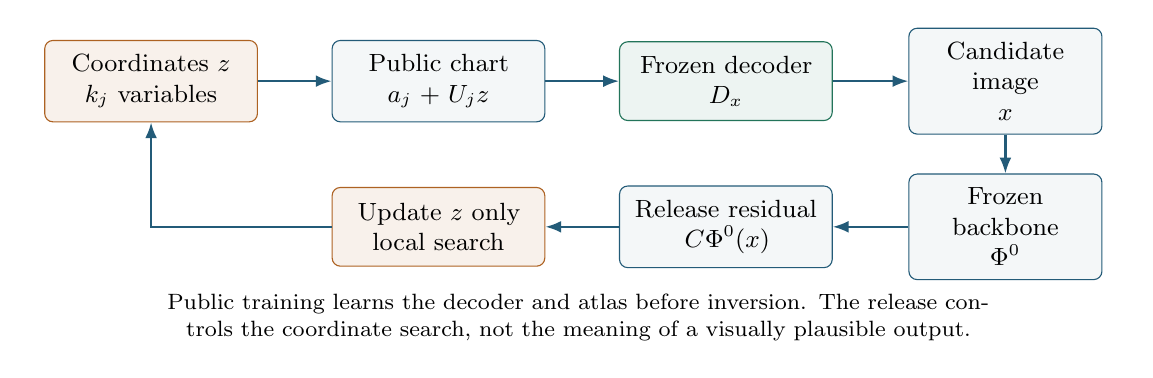
\begin{tikzpicture}
\node[free,text width=2.35cm] (z) at (0,0) {Coordinates $z$\\$k_j$ variables};
\node[box,text width=2.35cm] (lift) at (3.65,0) {Public chart\\$a_j+U_jz$};
\node[learn,text width=2.35cm] (dec) at (7.3,0) {Frozen decoder\\$D_x$};
\node[box,text width=2.1cm] (x) at (10.85,0) {Candidate image\\$x$};
\node[box,text width=2.1cm] (phi) at (10.85,-1.85) {Frozen backbone\\$\Phi^0$};
\node[box,text width=2.35cm] (res) at (7.3,-1.85) {Release residual\\$C\Phi^0(x)$};
\node[free,text width=2.35cm] (opt) at (3.65,-1.85) {Update $z$ only\\local search};
\draw[arr] (z)--(lift);\draw[arr] (lift)--(dec);\draw[arr] (dec)--(x);
\draw[arr] (x)--(phi);\draw[arr] (phi)--(res);\draw[arr] (res)--(opt);
\draw[arr] (opt.west)-|(z.south);
\node[font=\footnotesize,align=center,text width=13.7cm] at (5.4,-3.0) {Public training learns the decoder and atlas before inversion. The release controls the coordinate search, not the meaning of a visually plausible output.};
\end{tikzpicture}
\caption{Image-side architecture. Orange boxes change during inversion; green denotes a publicly learned, frozen network. Replay can consume the same candidate image through a separate residual branch.}
\label{fig:imagechart}
\end{figure}

\subsection{A feature chart is faster, but its decoder is a second inverse problem}

\begin{proposal}[Public feature autoencoder and image readout]\label{pr:featurebuild}
For public images $x_a$, $a=1,\ldots,P_{\rm pub}$, compute $h_a=\Phi^0(x_a)\in\R^n$. Train an encoder $E_h:\R^n\to\R^d$ and decoder $D_h:\R^d\to\R^n$ using, for example,
\[
\mathcal L_h=\frac1{P_{\rm pub}}\sum_{a=1}^{P_{\rm pub}}
\norm{D_h(E_h(h_a))-h_a}^2+\lambda_h\mathcal R_h.
\]
Here $\mathcal R_h$ is an explicitly chosen regularizer and $\lambda_h\ge0$ its weight. A small multilayer perceptron can implement each map when the layer features are vectors. Freeze both, form $\psi_j(w)=D_h(a_j+U_jw)$, and optimize $C\psi_j(w)$. This avoids the image decoder and backbone in the inner certificate loop.

A readout network $D_{\rm img}:\R^n\to\R^D$ must be trained on the public pairs $(h_a,x_a)$, or otherwise be demonstrably compatible with these features. A proposed readout loss may combine a pixel term, a fixed perceptual embedding $\Pi:\R^D\to\R^{d_\Pi}$, and a feature-cycle term:
\[
\begin{aligned}
\mathcal L_{\rm read}=\frac1{P_{\rm pub}}\sum_a
\bigl[&\lambda_x\norm{D_{\rm img}(h_a)-x_a}^2\\
&+\lambda_\Pi\norm{\Pi(D_{\rm img}(h_a))-\Pi(x_a)}^2\\
&+\lambda_\Phi\norm{\Phi^0(D_{\rm img}(h_a))-h_a}^2\bigr].
\end{aligned}
\]
The three nonnegative weights are design choices, not a theorem that all terms can vanish. If $\Phi^0$ loses information, a stochastic conditional decoder represents multiple possible images; its random seed is not recovered evidence unless separately identified.

Finally re-encode $\widehat x=D_{\rm img}(\widehat h)$ and report both $\norm{\Phi^0(\widehat x)-\widehat h}$ and the certificate residual of $\Phi^0(\widehat x)$. Use the fast feature result to initialize an image-side chart when exact realizability matters. Theorem~\ref{thm:feature} states the conditions under which the two routes are equivalent.
\end{proposal}

\begin{figure}[htbp]
\centering
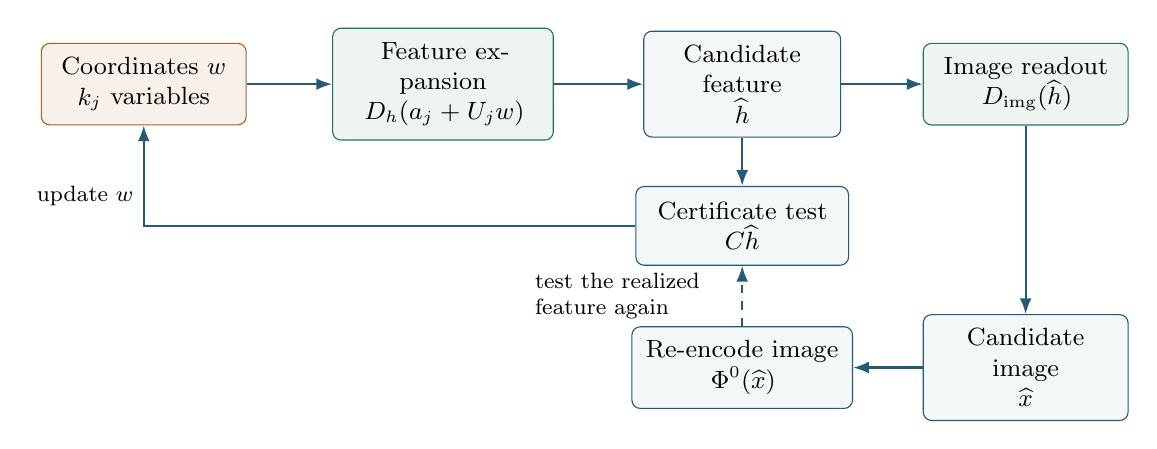
\begin{tikzpicture}
\node[free,text width=2.25cm] (w) at (0,0) {Coordinates $w$\\$k_j$ variables};
\node[learn,text width=2.45cm] (dh) at (3.8,0) {Feature expansion\\$D_h(a_j+U_jw)$};
\node[box,text width=2.15cm] (h) at (7.6,0) {Candidate feature\\$\widehat h$};
\node[box,text width=2.35cm] (cert) at (7.6,-1.8) {Certificate test\\$C\widehat h$};
\node[learn,text width=2.25cm] (dx) at (11.2,0) {Image readout\\$D_{\rm img}(\widehat h)$};
\node[box,text width=2.25cm] (xout) at (11.2,-3.6) {Candidate image\\$\widehat x$};
\node[box,text width=2.45cm] (cycle) at (7.6,-3.6) {Re-encode image\\$\Phi^0(\widehat x)$};
\draw[arr] (w)--(dh);\draw[arr] (dh)--(h);\draw[arr] (h)--(cert);
\draw[arr] (cert.west)-|node[pos=.65,left,font=\footnotesize] {update $w$}(w.south);
\draw[arr] (h)--(dx);\draw[arr] (dx)--(xout);
\draw[arr] (xout)--(cycle);
\draw[arr,dashed] (cycle)--node[left,font=\footnotesize,text width=2.5cm] {test the realized\\feature again}(cert);
\end{tikzpicture}
\caption{Feature-side architecture. The fast optimization loop and the image readout are separate. A plausible decoded image is not enough: the feature it actually produces must be checked. The outer path supplies the readout; dashed arrows denote validation.}
\label{fig:featurechart}
\end{figure}

\subsection{Three quantities to optimize, rather than one attractive picture}

\begin{definition}[Coverage, plausibility, and evidence]
For a fixed chart and true image $x_*$, its coverage error is
$\delta_j=\inf_z\norm{G_j(z)-x_*}$. This is unknown during a real attack; held-out public data only provide a distribution-dependent proxy. Plausibility is a property of the prior or a separately specified perceptual criterion. Evidence is the residual and conditioning of the actual released observation on the chart. Neither a good perceptual score nor small $\delta_j$ on unrelated public images proves private-example recovery.
\end{definition}

\begin{proposition}[Resolution does not create identified detail]\label{prop:qualityfiber}
Let $\mathcal O:\R^D\to\R^a$ be the complete observation map used by an attack. Suppose $x_1\ne x_2$ are both plausible candidates and $\mathcal O(x_1)=\mathcal O(x_2)$. Every deterministic estimator based only on that observation and the same public information returns the same estimate in these two cases. Its worst-case error is at least $\norm{x_1-x_2}/2$.
\end{proposition}
\begin{proof}
The estimator's inputs are identical, so its output is a common point $\widehat x$. The triangle inequality gives
$\norm{x_1-x_2}\le\norm{x_1-\widehat x}+\norm{\widehat x-x_2}$.
At least one term is at least half the left side. No distributional or optimization assumption is used.
\end{proof}

Thus super-resolution or a sharper decoder can improve the appearance of a reconstruction while leaving its identity uncertainty unchanged. The appropriate output may be a family of observation-consistent images with common supported structure, not one increasingly confident rendering of unsupported detail.

\FloatBarrier
\clearpage
\section{The image-chart literature: architectures, training, and reuse}\label{sec:architectures}

\chapterbrief
{The building blocks already exist: neural atlases, autoencoders, GAN latents, diffusion codecs, and retrieval-conditioned generators. Their training objectives and domains differ. None turns its advertised latent width into a theorem about how many coordinates recover a private image.}
{Begin with the closest inverse-problem precedents, then choose an expansion architecture and identify exactly what was trained, what is frozen, and what is optimized. Text retrieval and image decoding play different roles; the two-stage diffusion illustration makes that separation explicit.}
{A decoder maps latent coordinates to images or features. An encoder supplies public codes or initializations. A prior constrains plausible outputs. Optimized noise or network weights count as unknowns even when an architecture is described as low-dimensional.}

The entries below are selected for this inversion problem. They are not a ranking of contemporary image-generation quality. Each separates what the cited work supplies from what still needs to be built for LoRA inversion. A neural decoder is an expansion map; it is a mathematical local chart only on neighborhoods where it is sufficiently regular and locally injective.

\begin{remark}[Match the architecture to the regularity assumptions]
The smooth-chart theorems are not automatically theorems about every neural implementation. A direct feature atlas can use smooth activations. For an image-side chart, the composition through the frozen backbone must also have the stated regularity. ReLU networks are smooth inside fixed activation regions, but a global statement including their boundaries needs a separate piecewise-smooth or stratified argument. Hard vector quantization is a discrete operation, not a smooth map with an informative ordinary Jacobian. Use a continuous codec for the differential analysis, or explicitly model the discrete branches. Freezing a sampler's randomness makes it deterministic; it does not by itself prove immersion or the required smoothness.
\end{remark}

\subsection{The closest inverse-problem precedents}

\begin{literature}[Generative priors for compressed sensing]\label{lit:bora}
Bora, Jalal, Price, and Dimakis~\cite{bora} optimize a pretrained generator's latent coordinates to fit linear measurements. Their theory uses a set-restricted lower bound on differences of generated signals, not merely tangent rank. For a Lipschitz generator on a bounded latent ball, independent Gaussian sensing admits guarantees whose measurement requirement depends on latent dimension and a logarithm involving Lipschitz constant, radius, and approximation tolerance. Recovery error includes generator representation error, observation noise, and optimization error.

\textbf{Use here.} This is the direct precedent for replacing pixels by $G(z)$. It also explains why a theorem about a local Jacobian is weaker than a theorem about all secants. Its independent sensing result cannot be transferred verbatim to $C$: the LoRA certificate is constrained to annihilate $\HH$, and its zero set necessarily includes span alternatives. Sections 1--3 address that distinction.
\end{literature}

\begin{literature}[Mixtures of VAEs explicitly used as charts for inversion]\label{lit:mixture}
Alberti, Hertrich, Santacesaria, and Sciutto~\cite{mixturevae} learn a mixture of VAE components, each representing one chart, and minimize an inverse-problem fidelity term over the learned manifold. Their construction uses injective linear expansions and invertible neural transformations to obtain injective decoders with explicit left inverses. Training includes likelihood-based component and mixture-weight learning; manifold optimization uses a Riemannian gradient method.

\textbf{Use here.} This is the closest architectural and mathematical template for a feature-space atlas, particularly when explicit coordinate transitions and inverse maps matter. Replacing their physical forward operator by the certificate or replay residual is a proposed specialization, not a new general atlas-inversion principle. The published image settings do not establish coverage of arbitrary photographs of a privately named subject.
\end{literature}

\subsection{Autoencoders, VAEs, and explicit multi-chart networks}

\begin{literature}[A VAE gives a learned decoder, not a discovered exact dimension]\label{lit:vae}
Kingma and Welling~\cite{vae} train an approximate posterior $q_\varphi(u\mid x)$ and a generative likelihood $p_\theta(x\mid u)$ by a variational bound. With prior $p(u)$, the minimized negative bound is
\[
\mathcal L_{\rm VAE}(x)=
\E_{u\sim q_\varphi(\cdot\mid x)}[-\log p_\theta(x\mid u)]
\operatorname{KL}(q_\varphi(u\mid x)\Vert p(u)).
\]
The encoder supplies coordinates and the decoder mean supplies a deterministic expansion. The latent width is an architectural choice. If the likelihood has full-dimensional output noise, its distribution is not supported on the decoder-mean manifold.

\textbf{Use here.} Train this model on public images, or on public backbone features with a suitable likelihood. Freeze the decoder and inspect local immersion, coverage, and the certificate Jacobian separately. The KL term does not prove that semantic factors are disentangled or that its chosen latent width is the private chart dimension.
\end{literature}

\begin{literature}[Generative Latent Optimization]\label{lit:glo}
Bojanowski, Joulin, Lopez-Paz, and Szlam~\cite{glo} train a convolutional generator jointly with a separate latent code for each public training example, using reconstruction losses instead of an adversarial discriminator. In schematic notation, with public images $x_a$,
\[
\min_{\theta,\{u_a\}}\ \sum_a\ell(D_\theta(u_a),x_a),
\]
subject to the model's latent-code constraints.

\textbf{Use here.} This suggests a direct way to learn a sectional expansion on public examples when a separate encoder is unnecessary. After training, freeze $\theta$, keep the learned codes as anchors, and fit local coordinates around them. Public reconstruction alone does not ensure good interpolation between anchors or generalization to a private subject; those are additional requirements.
\end{literature}

\begin{literature}[Chart Auto-Encoders]\label{lit:chartae}
Schonsheck, Chen, and Lai~\cite{chartae} explicitly replace one flat latent representation by multiple chart encoders and decoders plus a chart predictor. Their training combines reconstruction, prediction of chart assignments, and Lipschitz-oriented regularization. They initialize charts around separated public examples and discuss local PCA initialization and transition maps on overlaps.

\textbf{Use here.} This directly supports learning overlapping local patches instead of forcing every viewpoint or subject into one coordinate system. Their approximation theory is conditional on a manifold model; it does not show that an arbitrary natural-image distribution is one smooth manifold. Nor does a learned atlas automatically avoid intersections with $\HH$ other than private points.
\end{literature}

\begin{figure}[htbp]
\centering
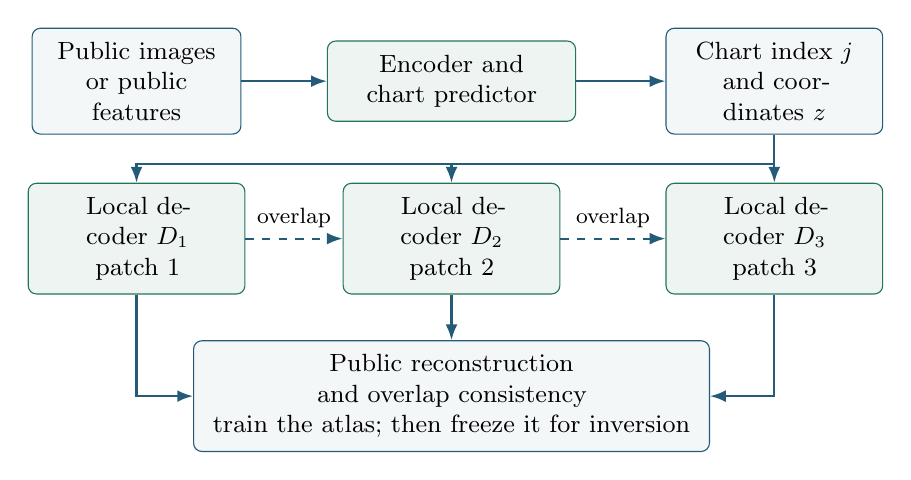
\begin{tikzpicture}
\node[box,text width=2.3cm] (data) at (0,0) {Public images\\or public features};
\node[learn,text width=2.8cm] (enc) at (4.0,0) {Encoder and\\chart predictor};
\node[box,text width=2.4cm] (assign) at (8.1,0) {Chart index $j$\\and coordinates $z$};
\node[learn,text width=2.4cm] (d1) at (0,-2) {Local decoder $D_1$\\patch 1};
\node[learn,text width=2.4cm] (d2) at (4,-2) {Local decoder $D_2$\\patch 2};
\node[learn,text width=2.4cm] (d3) at (8.1,-2) {Local decoder $D_3$\\patch 3};
\node[box,text width=6.2cm] (loss) at (4,-4) {Public reconstruction and overlap consistency\\train the atlas; then freeze it for inversion};
\draw[arr] (data)--(enc);\draw[arr] (enc)--(assign);
\draw[arr] (assign.south)--(d3.north);
\draw[arr] (assign.south)--(8.1,-1.05)-|(d2.north);
\draw[arr] (assign.south)--(8.1,-1.05)-|(d1.north);
\draw[arr] (d1.south)|-(loss.west);\draw[arr] (d2)--(loss);\draw[arr] (d3.south)|-(loss.east);
\draw[arr,dashed] (d1)--node[above,font=\footnotesize] {overlap}(d2);
\draw[arr,dashed] (d2)--node[above,font=\footnotesize] {overlap}(d3);
\end{tikzpicture}
\caption{Schematic multi-chart training architecture, motivated by \cite{chartae,mixturevae}; it is not a reproduction of either paper's exact implementation. Multiple decoders cover a union of patches. Overlap is useful for coordinate transitions; a mixture's discrete component is not an extra continuous image direction.}
\end{figure}

\subsection{StyleGAN: an efficient nonlinear expansion with a domain limitation}

\begin{literature}[StyleGAN and StyleGAN2]\label{lit:stylegan}
StyleGAN~\cite{stylegan} maps an input code through a mapping network into a style space, then uses styles at multiple synthesis layers together with separate stochastic noise. It is trained adversarially on an image collection. StyleGAN2~\cite{stylegan2} modifies synthesis and normalization and introduces path-length regularization to encourage a better-behaved latent-to-image mapping.

\textbf{Use here.} A pretrained generator whose training domain covers the subject is a relatively direct decoder $D_x$. Encode or optimize public examples into its style coordinates, then fit small local slices. Path-length regularization concerns the generator; it does not bound $\smin(CD\Phi^0DG_j)$.

The conventional $512$-coordinate style vector is not proof that a subject manifold has dimension $512$. Independently optimizing one style vector for each of $b_{\rm style}$ layers gives up to $512b_{\rm style}$ coordinates before any further restrictions; optimizing spatial synthesis noise adds still more. Fixing those quantities can reduce representation coverage. A face-domain checkpoint is not, merely by virtue of being StyleGAN, a motorcycle decoder.
\end{literature}

\begin{literature}[GANSpace and inversion encoders]\label{lit:gancontrols}
GANSpace~\cite{ganspace} uses PCA in GAN latent or intermediate feature spaces to obtain editing directions, including layer-specific controls. This supplies candidate bases $U_j$ without retraining the generator; interpretable directions need not be exhaustive or independent under our observation.

The e4e encoder of Tov et al.~\cite{e4e} addresses real-image embedding into StyleGAN while balancing reconstruction, editability, and perceptual quality. It is useful for obtaining public anchors, not as a private-image estimator from an adapter. ReStyle~\cite{restyle} trains an encoder to iteratively predict corrections to an image's current latent reconstruction. Its refinement observes the original image as well as the current reconstruction.

\textbf{Use here.} An iterative LoRA chart selector would instead have the release residual and public context. ReStyle does not justify using a reconstruction as its own independent target; adapting its update principle to adapter observations requires new training pairs and validation.
\end{literature}

\subsection{Latent diffusion: separate the codec from the image prior}

\begin{literature}[The two stages of a latent diffusion model]\label{lit:ldm}
Rombach et al.~\cite{ldm} first train an image autoencoder using perceptual and patch-adversarial objectives with either mild KL regularization or vector quantization. A second network learns denoising in the compressed latent space; cross-attention supports conditioning such as text. The spatial codec and the denoising prior do different jobs.

\textbf{Use here.} The codec decoder can cheaply evaluate $G_j(z)=D_x(a_j+U_jz)$, but arbitrary codec latents need not be realistic. Alternatively, restrict the input of a frozen, fixed-step deterministic conditional sampler $S_c$:
\[
G_{c,j}(z)=D_x(S_c(a_j+U_jz)).
\]
This keeps the generative prior inside the chart but requires differentiating through the sampler. Its derivative, not the prompt length, determines observability.

A spatial latent of height $h_{\rm lat}$, width $w_{\rm lat}$, and channel count $c_{\rm lat}$ has $d=h_{\rm lat}w_{\rm lat}c_{\rm lat}$ scalar coordinates. For illustration, a $64\times64\times4$ tensor contains $16\,384$ coordinates; it is not a $4$-dimensional chart. This arithmetic is not an intrinsic-dimension estimate.
\end{literature}

\begin{figure}[htbp]
\centering
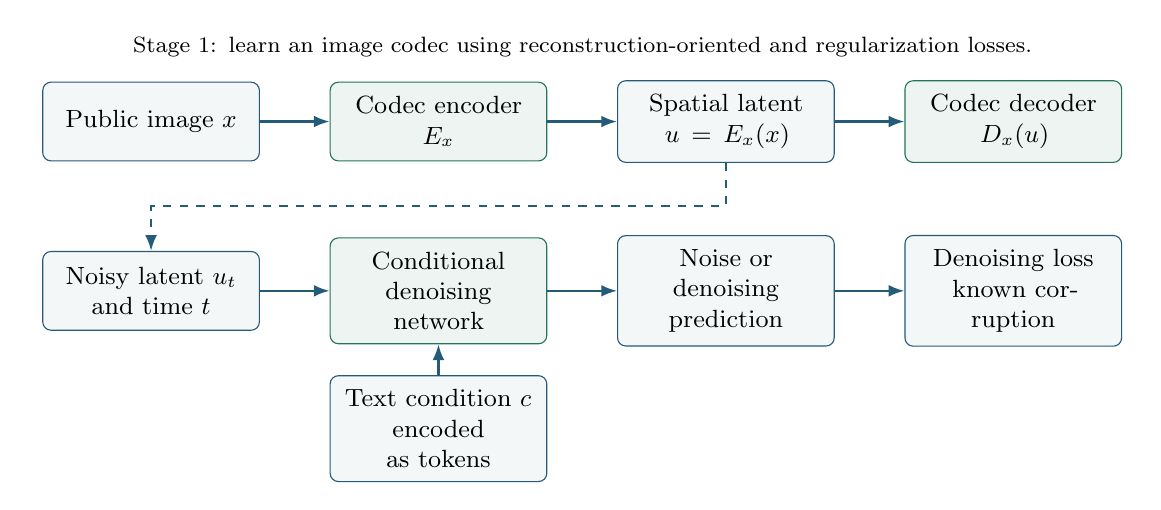
\begin{tikzpicture}
\node[box,text width=2.4cm] (x) at (0,0) {Public image $x$};
\node[learn,text width=2.4cm] (e) at (3.65,0) {Codec encoder\\$E_x$};
\node[box,text width=2.4cm] (u) at (7.3,0) {Spatial latent\\$u=E_x(x)$};
\node[learn,text width=2.4cm] (d) at (10.95,0) {Codec decoder\\$D_x(u)$};
\draw[arr] (x)--(e);\draw[arr] (e)--(u);\draw[arr] (u)--(d);
\node[font=\footnotesize,align=center,text width=13.8cm] at (5.45,.95) {Stage 1: learn an image codec using reconstruction-oriented and regularization losses.};
\node[box,text width=2.4cm] (noise) at (0,-2.15) {Noisy latent $u_t$\\and time $t$};
\node[box,text width=2.4cm] (c) at (3.65,-3.9) {Text condition $c$\\encoded as tokens};
\node[learn,text width=2.4cm] (net) at (3.65,-2.15) {Conditional\\denoising network};
\node[box,text width=2.4cm] (pred) at (7.3,-2.15) {Noise or\\denoising prediction};
\node[box,text width=2.4cm] (loss) at (10.95,-2.15) {Denoising loss\\known corruption};
\draw[arr] (noise)--(net);\draw[arr] (c)--(net);\draw[arr] (net)--(pred);\draw[arr] (pred)--(loss);
\draw[arr,dashed] (u.south)--++(0,-.55)-|(noise.north);
\end{tikzpicture}
\caption{The two-stage distinction in latent diffusion \cite{ldm}. This is a schematic training diagram, not a claim about a particular checkpoint's tensor sizes. A low-dimensional inversion chart must impose an additional coordinate restriction on the codec latent or sampler input.}
\end{figure}

\begin{proposal}[Three ways to reuse diffusion infrastructure]
\textbf{Fast codec chart.} Generate or retrieve public examples, encode them, and search a small neighborhood through the decoder only. Add a public latent-support constraint if interpolation leaves the learned image distribution.

\textbf{Sampler chart.} Fix the model, condition, numerical schedule, and any auxiliary randomness; optimize a small subspace of the sampler input. A nonlinear, deterministic expansion then exists, but computational cost can be substantial.

\textbf{Public distillation.} Train a fast student expansion $D_c^{\rm small}(z)$ on public subject-conditioned teacher outputs or public image/code pairs. Freeze it for inversion. Its approximation error is an extra contribution to $\delta$ in Theorem~\ref{thm:robust}. Teacher outputs can supply plausible variants, not guaranteed private training examples. None of these constructions receives a small $k$ merely from using a diffusion model.
\end{proposal}

\subsection{Text and retrieval identify candidate sections, not private photographs}

\begin{literature}[CLIP and retrieval-augmented generation]\label{lit:retrieval}
CLIP~\cite{clip} learns image and text encoders from paired image--text supervision using a contrastive matching objective. It provides a useful retrieval space for an adapter's declared label. It is not an image decoder, and its similarity is not a membership test.

Retrieval-Augmented Diffusion Models~\cite{rdm} condition a diffusion generator on representations of retrieved images. The retrieval database supplies visual information separately from the generator's fixed parameters.

\textbf{Use here.} A description can retrieve public motorcycles, which can anchor candidate chart families and conditioning sets. Querying for a narrower brand can propose more relevant anchors. Neither retrieval proximity nor semantic agreement with a generated candidate establishes that any retrieved photograph trained the adapter. Public images are prior-building material unless independently tested against the release.
\end{literature}

\begin{literature}[unCLIP is a decoder for a specific embedding]\label{lit:unclip}
Ramesh et al.~\cite{unclip} separate a prior over CLIP image embeddings, conditioned on text, from a diffusion decoder conditioned on those embeddings. This directly illustrates feature-to-image readout with generative uncertainty.

\textbf{Use here.} A recovered feature from an arbitrary internal layer of $\Phi^0$ is generally not a CLIP image embedding. One cannot feed it to unCLIP simply because both are vectors. A learned public bridge or a decoder trained for that exact feature space is needed, followed by re-encoding consistency checks. Even a perfectly compatible conditional decoder need not recover details discarded by its conditioning feature.
\end{literature}

\subsection{Untrained image priors: what is actually being optimized?}

\begin{literature}[Deep Image Prior and Deep Decoder]\label{lit:dip}
Deep Image Prior~\cite{dip} uses an untrained convolutional image-generating network and fits its weights to an image observation while holding an input code fixed. Its inductive bias comes from architecture and optimization, not from a pretrained subject distribution. The searched coordinates are the trainable weights, not the width of the fixed noise input.

Deep Decoder~\cite{deepdecoder} constructs images using repeated upsampling, channel mixing, nonlinearities, and normalization, with an underparameterized collection of weights. It offers a more explicit compact image representation without a public training corpus.

\textbf{Use here.} These are useful baselines or residual-detail models. They do not automatically isolate a named subject, and even an underparameterized decoder may have more independently varying coordinates than the certificate can identify. A low-dimensional weight subspace is another possible chart, but its coverage and Jacobian must be measured on that actual subspace.
\end{literature}

\begin{table}[htbp]
\centering
\small
\begin{tabular}{@{}Y{.19\textwidth}Y{.25\textwidth}Y{.22\textwidth}Y{.24\textwidth}@{}}
\toprule
Component & Public training or preparation & Fixed during inversion & Actual unknowns\\
\midrule
Feature autoencoder & Reconstruct $\Phi^0(x)$; optionally learn overlapping patches & Encoder, decoder, chart bank & Local feature coordinates\\[3pt]
StyleGAN slice & Adversarial generator training; public image inversion and local basis fitting & Generator and unsearched styles/noise & Selected style coordinates only\\[3pt]
Diffusion codec slice & Perceptual codec training; public latent neighborhoods & Codec decoder and atlas & Restricted spatial-latent coordinates\\[3pt]
Conditional sampler slice & Denoising training, with supported conditioning & Sampler weights, schedule, fixed conditioning and noise & Selected sampler-input coordinates\\[3pt]
Mixture of chart VAEs & Chart decoders, likelihood and mixture fitting & Learned atlas & Chart index plus local code\\[3pt]
Deep Image Prior & No public image pretraining required & Architecture and input code & Network weights that are fitted\\
\bottomrule
\end{tabular}
\caption{Training and inversion roles of the architectures discussed in Section~\ref{sec:architectures}. A fixed expansion's parameter count is not the latent search dimension.}
\end{table}

\textbf{Architecture choice for this thesis.} For the cleanest feature-level study, use a public feature autoencoder or an explicit multi-chart decoder. For image realization with a well-covered restricted domain, use a frozen image generator and local latent slices. For broad text-conditioned subjects, use a pretrained conditional generator to propose anchors, then decide explicitly whether the optimization runs through a fast codec or through the full sampler. This is a design recommendation, not a claim that one architecture has been experimentally established as best for LoRA inversion.

\FloatBarrier
\clearpage
\section{What is the dimension of the relevant image manifold?}\label{sec:dimension}

\chapterbrief
{There is no universal proved dimension for natural images. The useful quantity depends on family, scale, metric, and observation. Assess local reconstruction error and observation conditioning together; a narrower label need not lower dimension.}
{Separate the meanings of dimension, inspect the estimators and public-data protocol, then connect approximation error to coordinate-invariant sensitivity and chart count.}
{$k$ is searched dimension; $DG$ is the image tangent map; $M_G=DG^TDG$ measures image change. The private span rank $q$ is a different quantity.}

\subsection{There is no single number attached to natural images}

\begin{definition}[Five dimensions that must be kept separate]
At a candidate $x=G(z)$, distinguish:
\begin{enumerate}
\item ambient pixel dimension $D$, including channels;
\item a modeled local dimension $d_{\mathcal M}$ of a specified image family $\mathcal M$;
\item generator-coordinate width $d$, or restricted search width $k$;
\item local feature dimension $\rank(D\Phi^0(x)|_{T_x\mathcal M})$ when $\mathcal M$ is a smooth manifold;
\item observation rank $\rank D(F\circ G)(z)$, together with its conditioning in a specified image or feature metric.
\end{enumerate}
The private span rank $q$ is a sixth, different object: it is a linear-algebraic property of the private feature columns, not any of the dimensions above.
\end{definition}

\begin{proposition}[Why an exact image-manifold statement needs a model]
A finite set of quantized images has Hausdorff dimension zero. Conversely, adding independent, nondegenerate Gaussian pixel noise to any image distribution gives a distribution with support all of $\R^D$. Neither observation determines the useful low-dimensional structure at a nonzero reconstruction tolerance.
\end{proposition}
\begin{proof}
For any $s>0$, cover each of finitely many points by a ball of radius $\epsilon$. The sum of the $s$th powers of their diameters tends to zero as $\epsilon\downarrow0$, proving zero Hausdorff dimension. For the second assertion, every nonempty open ball has strictly positive Gaussian probability after translation by any fixed image. Averaging that positive conditional probability over the image law remains positive. Thus every open ball meets the support. The conclusions use finiteness and nondegenerate Gaussian noise respectively.
\end{proof}

In this project, a manifold is therefore a useful model of structured image variation at a chosen scale: for example, a fixed object's shape and appearance under pose, lighting, background, and crop changes. Different objects and occlusion regimes may require different patches or strata. A generator can cover such a family without being one globally injective coordinate chart.

\begin{proposition}[A narrower class label need not lower local dimension]\label{prop:labeldimension}
Let $\mathcal M$ be a smooth $d_{\mathcal M}$-dimensional image manifold, and let $b:\mathcal M\to\R$ be continuous. If a semantic section is $\mathcal M_b=\{x:b(x)>0\}$, then every $x\in\mathcal M_b$ has the same local manifold dimension and tangent space as in $\mathcal M$.

By contrast, if a section is the regular level set $g(x)=0$ for a $C^1$ map $g:\mathcal M\to\R^t$ whose differential has rank $t$ on that level set, its dimension is $d_{\mathcal M}-t$.
\end{proposition}
\begin{proof}
The strict inequality and continuity make $\mathcal M_b$ open in $\mathcal M$. Restrict any local coordinate chart to a sufficiently small neighborhood of $x$ contained in that open set; neither its dimension nor tangent changes. The second assertion is the regular-level-set theorem on $\mathcal M$, applied using the stated full-rank differential.
\end{proof}

\textbf{Interpretation.} Motorcycle versus Harley-Davidson can remove distant alternatives while retaining all local pose, illumination, and detail degrees of freedom. Fixing an actual shared identity parameter can reduce continuous dimension. A class label is not automatically such an equality constraint. Better semantic restriction can therefore improve search by reducing the number of plausible branches even when $k$ is unchanged.

\subsection{What the dimension-estimation papers actually provide}

\begin{literature}[Image datasets and network representations]\label{lit:imagedimension}
Pope et al.~\cite{pope} study intrinsic-dimension estimation specifically for image datasets, using nearest-neighbor estimators and controllable generative constructions to examine estimator behavior. This is a useful methodology reference, not a theorem assigning a universal dimension to unseen subject photographs.

Ansuini et al.~\cite{ansuini} apply intrinsic-dimension analysis to representations at different layers of image networks. Their nonlinear geometric viewpoint distinguishes curved low-dimensional representations from low-rank linear approximations.

\textbf{Use here.} Estimate separately on pixels, generator coordinates, and the actual frozen layer features. A dimension estimate from another backbone, a global dataset, or a different semantic mixture does not transfer to the chart tangent relevant to $C$. This note does not reproduce or assert any of these papers' numerical estimates.
\end{literature}

\begin{literature}[Nearest-neighbor dimension estimates]\label{lit:knn}
Levina and Bickel~\cite{levina} estimate intrinsic dimension using local neighbor-distance likelihoods. Write $T_j(x)$ for the distance to the $j$th neighbor of $x$ in a chosen metric, and let $b_{\rm nn}>2$ be a neighborhood count. One local likelihood form is
\[
\widehat d_{\rm nn}(x)=
\left[\frac1{b_{\rm nn}-1}\sum_{j=1}^{b_{\rm nn}-1}
\log\frac{T_{b_{\rm nn}}(x)}{T_j(x)}\right]^{-1}.
\]
Aggregation and bias corrections are separate estimator choices.

Facco et al.~\cite{twonn} use the ratio $\mu=T_2/T_1$. Under a locally homogeneous $d_{\mathcal M}$-dimensional Poisson model,
$\Prob(\mu\le u)=1-u^{-d_{\mathcal M}}$ for $u\ge1$.
Their method estimates dimension from this relationship.

\textbf{Use here.} These methods suggest a neighborhood-scale range for a public sectional chart. They depend on metric, sampling density, noise, boundaries, and scale; correlated or duplicate photographs do not supply independent geometric evidence. They do not test certificate identifiability.
\end{literature}

\begin{literature}[Diffusion models as dimension and tangent estimators]\label{lit:diffdimension}
Stanczuk et al.~\cite{stanczuk} connect small-noise diffusion scores to directions normal to a data manifold, providing a route to estimate tangent dimension from a trained model. Kamkari et al.~\cite{flipd} derive FLIPD using the Fokker--Planck equation associated with diffusion, targeting local intrinsic dimension with pretrained models.

\textbf{Use here.} These are directly relevant when a subject-conditioned image prior is already available: the prior may help propose a local tangent as well as render images. But estimates concern the learned distribution and noise scale. A general text-conditioned generator's local geometry need not be the geometry of the private subject, and a small estimated dimension does not establish good alignment with the certificate. Treat such estimates as model-dependent diagnostics, not a certified value of $k$.
\end{literature}

\subsection{A dimension protocol for the actual LoRA layer}

\begin{proposal}[Estimate a local operating dimension, not a universal image dimension]\label{pr:dimensionprotocol}
Use a public reference set for the declared section and keep separate held-out subjects or identities. For each anchor, vary a neighborhood radius and perform the following checks in a specified metric.
\begin{enumerate}
\item \textbf{Public geometric complexity.} Compute local PCA spectra and nearest-neighbor estimates in pixels, decoder latents, and the actual layer features. Normalize only if the eventual reconstruction problem uses that normalization. Record how the estimate changes with radius, noise, and near-duplicate removal.
\item \textbf{Coverage at a fixed budget.} For several $k$, fit public local charts and evaluate the held-out distance to their images. Fitting an encoder gives an upper bound on the best representation error through its reconstruction, not necessarily the exact distance.
\item \textbf{Generator geometry.} Inspect $DG_j$ or $D\psi_j$ for redundant coordinates and badly scaled directions. A high decoder-coordinate width can contain a much lower effective tangent rank.
\item \textbf{Observable geometry.} Evaluate the properly scaled certificate or stacked observation Jacobian on the candidate neighborhoods. Record singular values, not just rank. This step is release-dependent; the deterministic tests remain valid, but one cannot invoke a fixed-chart random law for arbitrary newly optimized charts.
\item \textbf{Resolution of the claim.} Choose the target error metric: layer-feature accuracy, pose/identity accuracy in a justified perceptual metric, or private-pixel accuracy. They require different coverage and injectivity assumptions.
\end{enumerate}
The output is a family of local triples $(k,\delta_{\rm public},\alpha)$ and usable radii, not one number advertised as the intrinsic dimension of the adapter's images.
\end{proposal}

\begin{proposition}[What local PCA measures]\label{prop:pcatail}
Let $y_a\in\R^b$, $a=1,\ldots,P_{\rm pub}$, be centered public vectors with covariance
$\Sigma_{\rm pub}=P_{\rm pub}^{-1}\sum_a y_ay_a^T$ and eigenvalues
$\lambda_1\ge\cdots\ge\lambda_b\ge0$. Among all orthogonal rank-$k$ projections $P$, the minimum mean squared projection error is
\[
\min_P\frac1{P_{\rm pub}}\sum_a\norm{y_a-Py_a}^2
=\sum_{j>k}\lambda_j.
\]
This is a finite-sample linear approximation statement, not an estimator theorem for a nonlinear manifold's dimension.
\end{proposition}
\begin{proof}
The objective equals $\tr\Sigma_{\rm pub}-\tr(P\Sigma_{\rm pub})$. In an eigenbasis of $\Sigma_{\rm pub}$, write $p_j=e_j^TPe_j$. An orthogonal rank-$k$ projection has $0\le p_j\le1$ and $\sum_jp_j=k$. Thus $\sum_j\lambda_jp_j\le\sum_{j\le k}\lambda_j$, with equality for the projection onto the first $k$ eigenvectors. Subtracting gives the formula.
\end{proof}

\begin{proposition}[Curvature and omitted directions set the local chart error]\label{prop:curvature}
Let $g:B(a,\rho)\subset\R^d\to\R^b$ be $C^1$ and suppose
$\norm{Dg(u)-Dg(v)}\le L_{\rm curv}\norm{u-v}$ on this ball. For an orthogonal projection $P$ onto a chosen $k$-dimensional latent subspace and $\norm v<\rho$,
\begin{align}
\norm{g(a+v)-g(a)-Dg(a)Pv}
&\le\norm{Dg(a)(I-P)v}+\tfrac12L_{\rm curv}\norm v^2,\label{eq:tangenterror}\\
\norm{g(a+v)-g(a+Pv)}
&\le\norm{Dg(a)(I-P)v}
+\tfrac12L_{\rm curv}(\norm v^2+\norm{Pv}^2).\label{eq:nonlinearerror}
\end{align}
\end{proposition}
\begin{proof}
The fundamental theorem of calculus gives
$g(a+v)=g(a)+Dg(a)v+e(v)$ with
$\norm{e(v)}\le\int_0^1L_{\rm curv}t\norm v^2\,dt
=L_{\rm curv}\norm v^2/2$.
Subtract the linear approximation with $Pv$ to prove \eqref{eq:tangenterror}. Apply the same formula to $Pv$ and subtract the two expansions to prove \eqref{eq:nonlinearerror}.
\end{proof}

With $g=D_x$, the second bound applies to the realistic nonlinear slice in \eqref{eq:decoderchart}; with $g=\Phi^0\circ D_x$, it applies in the certificate's feature space. Recentering can reduce the quadratic error by reducing the necessary radius. It cannot eliminate a missing first-order direction. Insert any resulting coverage bound into Theorem~\ref{thm:robust}; this gives the promised connection between the quality of the constructed chart and the reconstruction error.

\subsection{Measure sensitivity per unit image change}

\begin{figure}[htbp]
\centering
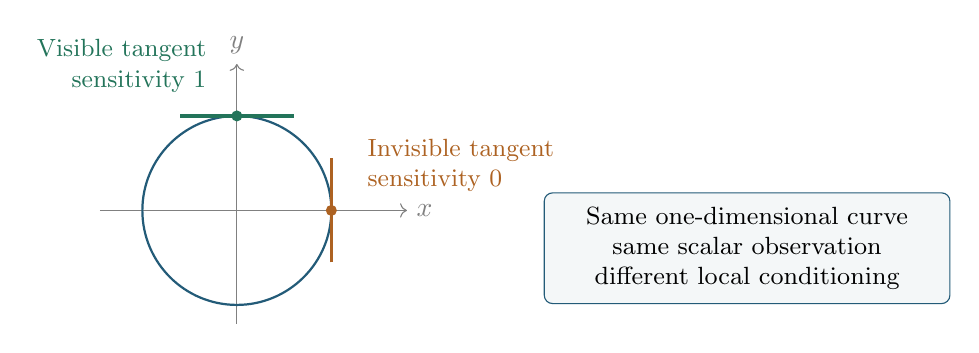
\begin{tikzpicture}[x=1.2cm,y=1.2cm]
\draw[->,gray] (-1.45,0) -- (1.8,0) node[right] {$x$};
\draw[->,gray] (0,-1.2) -- (0,1.55) node[above] {$y$};
\draw[thick,chartblue] (0,0) circle (1);
\draw[very thick,chartgreen] (-.6,1) -- (.6,1);
\draw[very thick,chartorange] (1,-.55) -- (1,.55);
\fill[chartgreen] (0,1) circle (2pt);
\fill[chartorange] (1,0) circle (2pt);
\node[font=\small,chartgreen,anchor=south east,align=right] at (-.22,1.15) {Visible tangent\\sensitivity $1$};
\node[font=\small,chartorange,anchor=west,align=left] at (1.28,.48) {Invisible tangent\\sensitivity $0$};
\node[box,text width=4.8cm] at (5.4,-.40) {Same one-dimensional curve\\same scalar observation\\different local conditioning};
\end{tikzpicture}
\caption{Dimension does not determine observability. For the unit-speed chart $g(t)=(\cos t,\sin t)$ and observation $F(x,y)=x$, the derivative is $-\sin t$ and its singular value is $|\sin t|$. It equals one at the top and zero at the rightmost point. This is an analytical illustration, not an image-manifold measurement.}
\label{fig:dimensionconditioning}
\end{figure}
\FloatBarrier

\begin{literature}[Generator geometry uses a pullback metric]
Shao, Kumar, and Fletcher~\cite{riemannian} study the Riemannian geometry induced by a differentiable generator, including intrinsic paths and transported tangent directions. The relevant geometric object is the metric induced on latent coordinates by their changes in the generated data, rather than raw Euclidean distance between arbitrary latent codes.

\textbf{Use here.} We use that viewpoint to prevent latent rescaling from masquerading as better certificate conditioning. The next proposition is the precise local calculation needed for this task.
\end{literature}

\begin{proposition}[Coordinate-invariant observable sensitivity]\label{prop:metric}
Let $G:\R^d\to\R^D$ be an immersion at $u$, let $F:\R^D\to\R^a$ be differentiable there, and put
\[
B=DG(u),\quad M_G=B^TB,\quad J_F=DF(G(u))B.
\]
For a positive definite residual weight matrix $W\in\R^{a\times a}$, define
\[
K=W^{1/2}J_FM_G^{-1/2}.
\]
The squared minimum observation change per unit infinitesimal image change is
\begin{equation}\label{eq:intrinsicmetric}
\alpha_{\rm image}^2
=\inf_{v\ne0}\frac{v^TJ_F^TWJ_Fv}{v^TM_Gv}
=\lambda_{\min}(K^TK).
\end{equation}
It is unchanged under an invertible change of local coordinates. A chosen positive semidefinite image metric may replace the pixel metric provided its pullback is positive definite on the selected tangent.
\end{proposition}
\begin{proof}
The immersion assumption makes $M_G$ positive definite. Substitute $t=M_G^{1/2}v$ into the quotient to obtain $\norm{Kt}^2/\norm t^2$, proving the formula. Under a local coordinate change with invertible derivative $S$, both quadratic forms change by congruence: $J_F^TWJ_F$ becomes $S^TJ_F^TWJ_FS$ and $M_G$ becomes $S^TM_GS$. Substitution $v=Sw$ preserves the set of quotient values. The same argument uses any positive definite pullback of a specified image metric.
\end{proof}

\begin{proposition}[The best locally observable $k$ directions]\label{prop:bestdirections}
Under Proposition~\ref{prop:metric}, let
$\lambda_1\ge\cdots\ge\lambda_d\ge0$ be the eigenvalues of $K^TK$. Among all $k$-dimensional tangent subspaces, the largest possible minimum squared observation sensitivity per unit image change equals $\lambda_k$. It is attained by the span of the first $k$ eigenvectors in the metric-normalized coordinates.
\end{proposition}
\begin{proof}
On the span of the first $k$ eigenvectors, every unit vector has quadratic form at least $\lambda_k$, with equality at the $k$th eigenvector. Conversely, any $k$-dimensional subspace intersects the span of eigenvectors $k,\ldots,d$ nontrivially, because the dimensions sum to $d+1$. A unit vector in that intersection has quadratic form at most $\lambda_k$. This proves both optimality and attainment.
\end{proof}

\textbf{Interpretation and obstacle.} This is an exact local answer to which $k$ directions are most measurable. It is not an instruction to discard every hard-to-measure direction: an omitted direction may be needed to represent the true image. Good chart construction trades this spectrum against coverage and semantics. Public variance PCA and observation sensitivity solve different optimization problems. When $K$ uses the released certificate, choosing a new basis from it is adaptive and does not inherit an unqualified fixed-chart probability guarantee.

\begin{definition}[A resolution-dependent observable dimension]
For a chosen sensitivity threshold $\tau>0$, define
$d_{\rm obs}(\tau)=|\{j:\lambda_j(K^TK)\ge\tau^2\}|$.
This is a deterministic local diagnostic in the chosen metrics. A noise tolerance and a desired image-error scale can motivate $\tau$; there is no universal numerical threshold. The count must be accompanied by coverage error and a neighborhood on which the derivative stays controlled.
\end{definition}

\subsection{Local dimension versus a global atlas}

\begin{proposition}[Chart count adds a separate covering cost]\label{prop:atlascover}
Suppose each $G_j:\overline B(0,\rho_j)\subset\R^{k_j}\to\R^D$ is $L_j$-Lipschitz and $\mathcal A$ is finite. Let $\mathcal N_\epsilon(S)$ be the least cardinality of an $\epsilon$-net of a set $S$ in Euclidean distance. Then
\[
\mathcal N_\epsilon(\mathcal M_{\mathcal A})
\le\sum_{j\in\mathcal A}\left(1+\frac{2L_j\rho_j}{\epsilon}\right)^{k_j}.
\]
When all $k_j=k$, $L_j\le L_*$ and $\rho_j\le\rho_*$, its logarithm is at most
$\log|\mathcal A|+k\log(1+2L_*\rho_*/\epsilon)$.
\end{proposition}
\begin{proof}
For $L_j>0$, a maximal $\epsilon/L_j$-separated collection in the compact latent ball is a net. The disjoint balls of half that radius around its points fit inside the ball of radius $\rho_j+\epsilon/(2L_j)$. Comparing $k_j$-dimensional volumes bounds its size by $(1+2L_j\rho_j/\epsilon)^{k_j}$. Lipschitz continuity sends this collection to an $\epsilon$-net of the chart image. A constant map requires one point. Union the nets and take logarithms to obtain the assertions.
\end{proof}

Thus a class label may reduce $\log|\mathcal A|$ without changing $k$. This can reduce the discrete search and multiple-testing burden. A covering bound alone is not a theorem that the actual certificate embeds the atlas; a lower bound on observation differences or the appropriate constrained-kernel theorem is still required.

\clearpage
\section{Smart charts: labels, refinement, and learning from adapters}\label{sec:smart}

\chapterbrief
{A label or rough reconstruction can propose a more useful chart, but it does not supply independent evidence about the private image. A prebuilt public atlas permits release-dependent selection while retaining the stated fixed-family guarantees. Learning the selector from many adapters needs genuine coverage supervision, not certificate fit alone.}
{Follow the motorcycle-to-brand proposal loop, then the fixed-atlas theorem. The coarse-to-fine rank test explains when extra controls add information. Shared-concept and public-adapter training proposals follow, together with their failure modes.}
{$G_c$ is a chart conditioned on a public concept $c$; $J_c,J_f$ measure coarse and fine coordinate changes. A fixed atlas is constructed before the release randomness; selecting an index is different from learning a new chart from that release.}

\subsection{A motorcycle-to-brand pipeline with an honest evidence loop}

\begin{proposal}[Hierarchical proposal and validation]\label{pr:hierarchy}
Parse the adapter description into separate hypotheses: object class, style, brand or identity, and nuisance attributes such as viewpoint. A style adapter need not represent one object, and an arbitrary trigger token need not have a meaningful public text embedding.

\begin{enumerate}
\item \textbf{Start from public candidates.} Retrieve diverse examples compatible with the label; include alternatives and an unknown-subject branch. Encode them into a fixed public generator or feature atlas. Keep separate charts for distinct pose and layout neighborhoods.
\item \textbf{Run a small-chart search.} Fit certificate coordinates inside each selected trust region. Keep residuals, singular values, and multiple candidate images. A rough reconstruction can supply a proposed semantic description.
\item \textbf{Branch instead of locking in.} If it suggests a motorcycle, propose cruiser, sport, touring, and alternative explanations as appropriate. If one branch suggests Harley-Davidson, retrieve brand-relevant public anchors while retaining visually similar brands and the broader fallback.
\item \textbf{Rebuild or reselect locally.} Prefer a prebuilt atlas subset when available. Otherwise fit new public-only anchors and tangent directions around the proposed section, declaring that their selection depended on the release. Recenter to reduce curvature error; do not force the next chart to contain the previous generated picture.
\item \textbf{Validate using the observation.} Test the new image through $\Phi^0$ and the release residual, with conditioning and mismatch tolerances. If independent, withheld observations exist, reserve them for selection checks. Add replay only with a justified training model.
\item \textbf{Stop at supported detail.} If several brands or identities remain observationally compatible, preserve those branches. Rendering a logo or finer texture is not grounds for asserting that it was present in a training image.
\end{enumerate}
\textbf{Kill criterion.} If refinement improves semantic confidence or sharpness without improving coverage diagnostics, observed fit, or distinguishability of competing hypotheses, it is a prior-driven rendering refinement, not improved private-data recovery.
\end{proposal}

\begin{figure}[htbp]
\centering
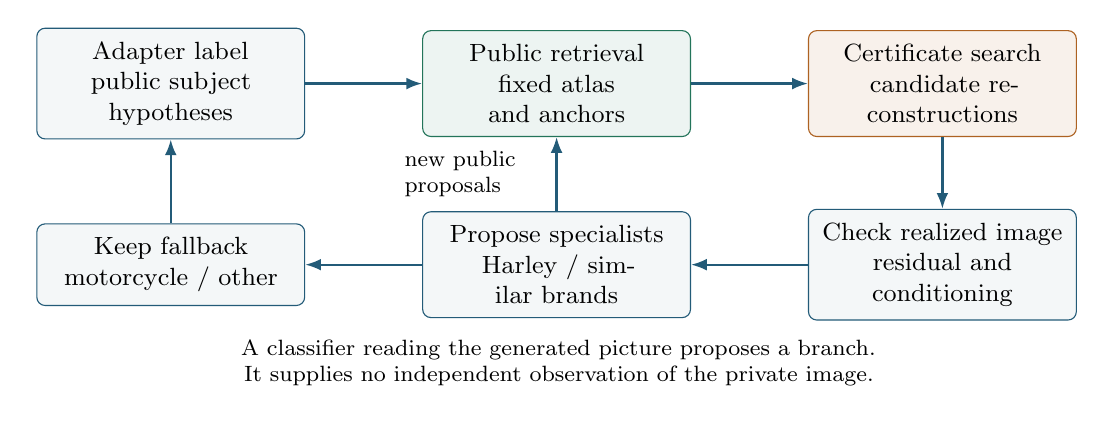
\begin{tikzpicture}
\node[box,text width=3.05cm] (label) at (0,0) {Adapter label\\public subject hypotheses};
\node[learn,text width=3.05cm] (bank) at (4.9,0) {Public retrieval\\fixed atlas and anchors};
\node[free,text width=3.05cm] (fit) at (9.8,0) {Certificate search\\candidate reconstructions};
\node[box,text width=3.05cm] (broad) at (0,-2.3) {Keep fallback\\motorcycle / other};
\node[box,text width=3.05cm] (narrow) at (4.9,-2.3) {Propose specialists\\Harley / similar brands};
\node[box,text width=3.05cm] (test) at (9.8,-2.3) {Check realized image\\residual and conditioning};
\draw[arr] (label)--(bank);\draw[arr] (bank)--(fit);\draw[arr] (fit)--(test);
\draw[arr] (test)--(narrow);\draw[arr] (narrow)--(broad);
\draw[arr] (narrow)--node[left,font=\footnotesize,text width=1.8cm] {new public\\proposals}(bank);
\draw[arr] (broad.north)--(label.south);
\node[font=\footnotesize,align=center,text width=13.2cm] at (4.9,-3.55) {A classifier reading the generated picture proposes a branch. It supplies no independent observation of the private image.};
\end{tikzpicture}
\caption{Subject refinement is hypothesis search with a fallback, not a chain of self-confirming labels. The release remains the evidence source at every level.}
\label{fig:hierarchy}
\end{figure}

\begin{proposition}[Changing coordinates or narrowing a set is not new information]\label{prop:refinement}
Let $\mathcal S$ be a candidate set and $\ell:\mathcal S\to[0,\infty)$ an observation loss. A bijective reparameterization preserves the infimum and candidate minimizers in image space. If $\mathcal S_{\rm child}\subset\mathcal S_{\rm parent}$, then
\[
\inf_{\mathcal S_{\rm child}}\ell\ \ge\ \inf_{\mathcal S_{\rm parent}}\ell.
\]
Further, if a proposed label is a deterministic function of the release and fixed public information, adding that label to an estimator's input does not distinguish any pair of datasets that gave identical original inputs.
\end{proposition}
\begin{proof}
A bijection preserves the values attained by $\ell$. The infimum over a subset cannot be smaller than that over its containing set. For the last assertion, identical release and public inputs produce identical proposed labels; any subsequent deterministic processing still has identical inputs. Randomized processing with the same conditional law likewise cannot distinguish the two cases through that extra label alone.
\end{proof}

\textbf{Why refinement can nevertheless help.} It can find a better optimization basin, replace a wrong chart by a nonnested better-covered chart, reduce the number of remote alternatives, or improve conditioning by restricting tangents. These are useful effects, but they are different from manufacturing new measurements. A decrease observed by an approximate optimizer on a nested child need not contradict the proposition: the parent optimization may simply have missed its optimum.

\begin{theorem}[Adaptive selection from a fixed public atlas]\label{thm:fixedatlas}
Fix $\HH$ and a finite or countable family of smooth feature charts $\{\psi_j\}_{j\in\mathcal A}$, independent of the initialization $A_0$. Suppose each satisfies the regularity assumptions of Theorem~\ref{thm:global} and has dimension $k_j<p=r-q$. In the same random-kernel setting, with probability one, simultaneously for all $j$,
\[
\im\psi_j\cap\ker C=\im\psi_j\cap\HH.
\]
Consequently an index chosen after observing $C$ from this fixed family still obeys the equality. This statement does not assert that the intersections contain only private points.
\end{theorem}
\begin{proof}
For each fixed $j$, Theorem~\ref{thm:global} supplies a probability-one event $E_j$ on which the equality holds on the entire chart. A finite or countable intersection of probability-one events still has probability one, since its complement is a countable union of null events. On that intersection the equality holds for every index, including any selected index. No independence between the events is required.
\end{proof}

This is a reason to separate public atlas construction from release-dependent chart selection. For nonzero residual thresholds, finite-family false-positive control needs a quantitative union bound, such as the bounds in Section 2, and a separation assumption. The countable probability-one statement alone gives no useful finite-noise threshold. Splitting rows of one certificate does not automatically create independent validation information.

\subsection{Allow fine detail only when it adds observable directions}

\begin{proposition}[A coarse-to-fine expansion test]\label{prop:coarsefine}
Let a chart have coarse coordinates $z_c\in\R^{k_c}$ and proposed fine coordinates $z_f\in\R^{k_f}$. At a fixed point let its residual derivative be $[J_c\ J_f]$, with $J_c\in\R^{a\times k_c}$ of full column rank and $J_f\in\R^{a\times k_f}$. Then
\[
\rank[J_c\ J_f]
=k_c+\rank((I-P_{\col J_c})J_f).
\]
Thus full first-order identification of both blocks holds exactly when the projected fine block has column rank $k_f$.
\end{proposition}
\begin{proof}
Decompose each column of $J_f$ into its orthogonal projection onto $\col J_c$ and its orthogonal complement. The first part adds no column direction beyond $J_c$, while the second is orthogonal to that column space. Their span dimensions therefore add.
\end{proof}

A positive but tiny smallest singular value of the projected block indicates fragile detail recovery; conditioning of the complete block, with the image metric of Proposition~\ref{prop:metric}, must still be checked. One can add pose and silhouette coordinates first, then candidate texture or background directions. This is a proposed ordering, not an assertion that every architecture cleanly separates those factors. Optimizing many fine-scale noise maps can improve appearance while making the inverse problem unidentifiable.

\subsection{A shared subject is not the same as independent image codes}

\begin{proposal}[Factor identity from per-image variation]\label{pr:sharedbuild}
Let $c$ denote a discrete public concept condition, $s\in\R^{d_s}$ a shared identity code, and $u_i\in\R^{d_i}$ a per-image code. Use a frozen conditional expansion
\[
x_i=G_c(s,u_i),\qquad i=1,\ldots,M.
\]
The ordered product parameterization has $d_s+\sum_i d_i$ continuous coordinates, compared with $\sum_i(d_s+d_i)$ if every image has an independent identity code. These are parameter counts, not an identifiability theorem. Theorem~\ref{thm:shared} gives the projected shared-versus-private Jacobian condition.

\textbf{Public training proposal.} Use public multi-view or same-identity groups to train one shared code with per-image reconstruction codes, adding the image or feature reconstruction losses from Section~\ref{sec:build}. Without grouping or other supervision, there is no reason the network must assign identity to $s$ rather than leak it into every $u_i$. Permutation, duplicate-image collapse, and generator coordinate symmetries must be handled explicitly.

\textbf{Kill criterion.} If the projected shared Jacobian is rank deficient, or if per-image codes can absorb all identity changes, the parameter-count saving does not yield identified shared information.
\end{proposal}

\subsection{Learning from thousands of adapters: a supervised route and a limit}

\begin{proposal}[Amortize chart selection using public adapter tasks]\label{pr:meta}
Fix the known base model. For public task index $t=1,\ldots,T_{\rm task}$, construct a public image set $\mathcal D_t$, a description $c_t$, and an adapter release $\mathcal R_t=(A_t,B_t)$ using a recorded recipe. For certificate training tasks, require the valid scalar-update setting and excitation/non-annihilation assumptions of this note. A collection of arbitrary released adapters, including ones trained outside that optimizer class, cannot automatically supply valid certificate examples.

Train a selector
\[
S_\theta:(\mathcal R_t,c_t)\longmapsto
\text{scores over a fixed public atlas, initial coordinates, and uncertainty}.
\]
An implementation can use a text encoder, an encoder of matrix summaries, and a small fusion network. Inputs may include singular spectra, the merged update, or the projector $C_t^\dagger C_t$ onto the certificate row space; the last is invariant to changing a basis of those certificate rows. Choice of representation is a design question, not a claimed universal invariance of arbitrary LoRA factorizations.

Because $\mathcal D_t$ is known in these public tasks, training can penalize actual coverage:
\[
\mathcal L_{\rm cover}(\theta)
=\sum_t\sum_{x\in\mathcal D_t}
\min_{\substack{j\in S_\theta(\mathcal R_t,c_t)\\ z\in K_j}}
\norm{G_j(z)-x}^2,
\]
where $K_j$ is the chart's fixed latent trust region and the selector returns a finite subset of indices. One may use a differentiable surrogate for the subset choice, but should retain held-out coverage as the criterion. Feature distances can replace pixel distances when that is the target. Record $q_t=\rank[\Phi^0(x)]_{x\in\mathcal D_t}$ rather than interpreting the image count as the certificate rank.

\textbf{What this buys.} The selector learns which public patches tend to explain which adapter observations, and can initialize local searches. The expensive reusable decoder is learned once. Subject-disjoint and recipe-shift validation are needed to distinguish transfer from memorizing a public dictionary.

\textbf{What is unproved.} Generalization to an unseen private identity; calibrated uncertainty under an unknown recipe; and the claim that a continuously synthesized release-dependent chart avoids false zeros. A selector of a fixed atlas has the clean guarantee of Theorem~\ref{thm:fixedatlas}; a hypernetwork that invents a new chart from the release needs a different analysis.
\end{proposal}

\begin{proposition}[Certificate-only meta-training cannot enforce image coverage]\label{prop:metacollapse}
Suppose a chart learner is trained solely to minimize
$\sum_t\sum_b\norm{C_t\psi_t(w_b)}^2$ at selected latent inputs $w_b$, without a noncollapse, reconstruction, or realizability constraint. The constant choice $\psi_t\equiv0$ attains the global minimum zero for every task. Excluding zero alone still does not distinguish private points from other admissible points in $\ker C_t$.
\end{proposition}
\begin{proof}
Every squared norm is nonnegative and $C_t0=0$, so the constant map achieves the smallest possible sum. For the second assertion, the loss is zero at every permitted kernel point, independent of whether it was a private example. The loss has no term separating those points.
\end{proof}

\begin{proposition}[Unpaired normalized certificates do not determine subject instances]\label{prop:metalimitation}
In the normalized Gaussian kernel model of Section 2, suppose two data-generating explanations give the same private spans $\HH_t$ and the same public descriptions for every task, but different private points within those spans. They induce the same joint law of independently initialized normalized certificates. No learner using only those certificates and descriptions can identify which explanation supplied the points.
\end{proposition}
\begin{proof}
For each fixed span, the quotient construction in Section 2 makes the normalized row-space law depend only on that span. Therefore the two explanations give the same law task by task; independence makes the joint laws equal. Any measurable learner applied to inputs with equal laws has the same output law. It cannot reliably distinguish the two explanations from those inputs alone.
\end{proof}

This does not rule out learning useful adapter clusters, learning with paired public tasks, or exploiting extra information in the full endpoints. It rules out inferring individual photographs merely by accumulating more observations whose statistical content is only a collection of spans.

\subsection{A release-adaptive alternative with a clear boundary}

\begin{proposal}[Use the model as a proposal source, then validate]\label{pr:selfproposal}
If the adapted model is itself generative, its samples can suggest class, shape, style, or identity hypotheses and public retrieval queries. Their use may be computationally valuable even though they are functions of the released model and fresh random seeds.

Fit candidate public charts around the proposed concepts, search them against the certificate, and distinguish proposal randomness from identified image coordinates. Generated samples are not independent additional measurements of the training set, and a generator's memorization behavior is not assumed. The deterministic composition and conditioning theorems still apply to any particular proposed chart; the fixed-chart random guarantees require the independence or finite-bank conditions already stated.
\end{proposal}

\FloatBarrier
\clearpage
\section{A multiscale geometric skeleton: local charts on a hierarchy}\label{sec:multiscale}

\chapterbrief
{The spider-web idea becomes a hierarchy of local charts: choose a region, then estimate a few coordinates inside it. Hierarchical storage can be cheap, but fine-scale coverage may still be expensive. Valid certificate bounds can discard entire branches; the number of surviving branches determines whether the hierarchy accelerates inversion.}
{Distinguish coverage nets, distance-preserving spanners, and continuous patches. The series and covering proofs quantify representation cost; the pruning proof gives a safe search rule. Architecture choices, public-data requirements, and the novelty assessment close the chapter.}
{$E$ counts finest-level patches, not private images; $\rho_a$ bounds a node's feature radius; $\ell_a$ is its residual lower bound; $\eta$ is the allowed residual. Each local chart has its own searched dimension $k_a$.}

The geometric picture is a collection of coarse regions, finer regions inside them, and connections that permit navigation without representing every image separately. Each level approximates the candidate family more accurately. A region contains a small expansion map, so it represents continuously many candidates rather than only a stored example. This section integrates the geometric intuition with the practical assessment: what already exists, what could help LoRA inversion, which architecture to put at a node, and which public data could support it.

\subsection{Nets, a sparse web, and an atlas preserve different things}

\begin{definition}[Three parts of the construction]\label{def:multiscaleobjects}
Let $(\mathcal M,d_{\mathcal M})$ be a compact metric space modeling an image or feature family. An $\varepsilon$-net is a finite subset $S\subseteq\mathcal M$ such that every point of $\mathcal M$ lies within distance $\varepsilon$ of some point of $S$. A hierarchy uses such representatives at decreasing resolutions, with finer regions assigned to coarser parents. On a finite representative set $S$, a weighted graph is a $(1+\theta)$-spanner, for $\theta\ge0$, if its shortest-path distance $d_{\rm graph}$ satisfies
\[
d_{\mathcal M}(a,b)\le d_{\rm graph}(a,b)
\le(1+\theta)d_{\mathcal M}(a,b)\qquad(a,b\in S).
\]
An atlas additionally assigns each region a local parameterization and a bounded coordinate domain. Neither the existence of a hierarchy nor the attachment of charts implies the spanner inequalities.
\end{definition}

\begin{center}
\small
\begin{tabular}{@{}Y{.27\textwidth}Y{.25\textwidth}Y{.38\textwidth}@{}}
\toprule
Geometric intuition & Mathematical object & What it supplies\\
\midrule
Representatives at finer scales & Hierarchical nets / net trees & Coverage at each resolution\\[4pt]
A sparse spider web & A geometric spanner & Controlled travel distances between representatives\\[4pt]
A patch around each representative & A multiscale atlas & Continuous local approximation and coordinates\\
\bottomrule
\end{tabular}
\end{center}

\begin{literature}[The direct precedents]\label{lit:gmra}
Har-Peled and Mendel~\cite{nettree} construct hierarchical nets in finite metrics of constant doubling dimension and use them for proximity search, spanners, and compact representations. Allard, Chen, and Maggioni~\cite{gmra} construct Geometric Multi-Resolution Analysis (GMRA): data-dependent multiscale dictionaries for point clouds with low-dimensional geometric structure. This is a particularly direct precedent for attaching local approximations to regions of a hierarchy. A hierarchy organizes refinement; additional neighbor connections can support navigation. Distance preservation requires its own construction and assumptions. No such guarantee for natural-image perceptual distances is assumed here.
\end{literature}

\begin{figure}[htbp]
\centering
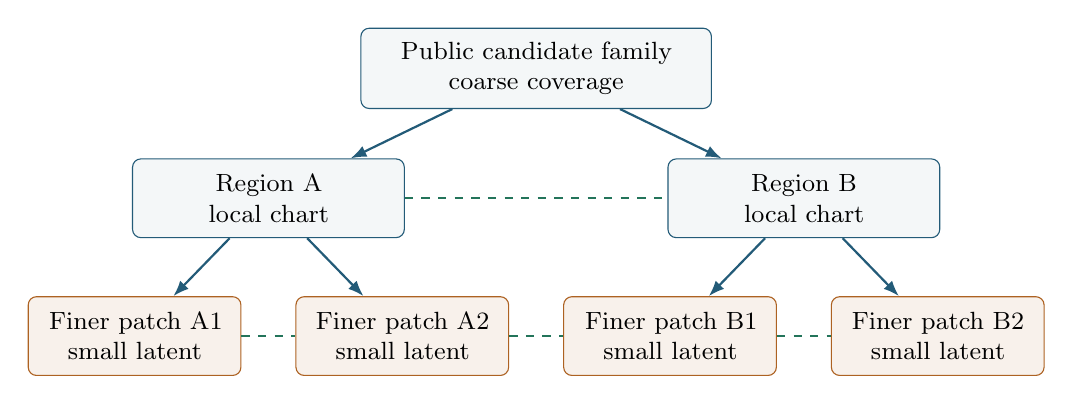
\begin{tikzpicture}
\node[box,text width=4.1cm] (root) at (0,0) {Public candidate family\\coarse coverage};
\node[box,text width=3.1cm] (left) at (-3.4,-1.65) {Region A\\local chart};
\node[box,text width=3.1cm] (right) at (3.4,-1.65) {Region B\\local chart};
\node[free,text width=2.35cm] (a1) at (-5.1,-3.4) {Finer patch A1\\small latent};
\node[free,text width=2.35cm] (a2) at (-1.7,-3.4) {Finer patch A2\\small latent};
\node[free,text width=2.35cm] (b1) at (1.7,-3.4) {Finer patch B1\\small latent};
\node[free,text width=2.35cm] (b2) at (5.1,-3.4) {Finer patch B2\\small latent};
\draw[arr] (root) -- (left);
\draw[arr] (root) -- (right);
\draw[arr] (left) -- (a1);
\draw[arr] (left) -- (a2);
\draw[arr] (right) -- (b1);
\draw[arr] (right) -- (b2);
\draw[dashed,thick,draw=chartgreen] (left.east) -- (right.west);
\draw[dashed,thick,draw=chartgreen] (a1.east) -- (a2.west);
\draw[dashed,thick,draw=chartgreen] (a2.east) -- (b1.west);
\draw[dashed,thick,draw=chartgreen] (b1.east) -- (b2.west);
\end{tikzpicture}
\caption{A hierarchy of local charts. Solid arrows organize refinement; dashed links connect neighboring regions. Certificate bounds screen entire branches. The picture illustrates a design, not a proved spanner or an assumption of exact fractal self-similarity.}
\label{fig:multiscaleweb}
\end{figure}
\FloatBarrier

\subsection{The geometric series is cheap; the finest cover may be large}

\begin{proposition}[Storage overhead under geometric shrinkage]\label{prop:treestorage}
Let $E$ be the number of finest-level nodes. Suppose the number $E_j$ of nodes at the $j$-th coarser level satisfies $E_j\le E/2^j$ for $j=0,\ldots,J$, where $J$ is the maximum coarsening level. Then
\[
\sum_{j=0}^{J}E_j<2E,
\qquad
\sum_{j=1}^{J}jE_j\le2E.
\]
Thus a fixed storage cost per node, or a cost proportional to $j$ on coarser levels, has total order $E$. This counts node costs under the assumption; it does not bound unrestricted neighbor edges or separately trained network sizes.
\end{proposition}
\begin{proof}
The first sum is at most $E\sum_{j=0}^{J}2^{-j}<2E$. For the second, use nonnegative summation to obtain
\[
\sum_{j=1}^{\infty}j2^{-j}
=\sum_{t=1}^{\infty}\sum_{j=t}^{\infty}2^{-j}
=\sum_{t=1}^{\infty}2^{1-t}=2.
\]
Multiplying by $E$ proves the bound. The hypothesis is precisely the required geometric shrinkage; an arbitrary sampled hierarchy need not satisfy it.
\end{proof}

The hierarchy can therefore cost only a constant factor more than its finest level. The unresolved question is how many finest-level representatives are needed. Define the covering number
\[
\mathcal N(\mathcal M,\varepsilon)
=\min\bigl\{|S|:S\subseteq\mathcal M\text{ is an }\varepsilon\text{-net}\bigr\}.
\]
A representation by stored points alone needs $E\ge\mathcal N(\mathcal M,\varepsilon)$ for worst-case error at most $\varepsilon$.

\begin{proposition}[A precise setting for dimension-dependent coverage]\label{prop:coverdimension}
Assume $\mathcal M$ carries a finite measure $\nu$ with $V=\nu(\mathcal M)>0$. For some constants $c_-,c_+,t_0,d_*>0$, assume every open metric ball satisfies
\[
c_-t^{d_*}\le\nu(B_{\mathcal M}(x,t))\le c_+t^{d_*}
\quad(x\in\mathcal M,\ 0<t\le t_0).
\]
Then, for $0<\varepsilon<t_0$,
\[
\frac{V}{c_+\varepsilon^{d_*}}
\le\mathcal N(\mathcal M,\varepsilon)
\le\frac{2^{d_*}V}{c_-\varepsilon^{d_*}}.
\]
\end{proposition}
\begin{proof}
If $S$ is an $\varepsilon$-net, its closed $\varepsilon$-balls cover $\mathcal M$. Each such ball has measure at most $c_+\varepsilon^{d_*}$: apply the assumed upper bound to open balls of radius decreasing to $\varepsilon$ and use continuity of a finite measure from above. Summing gives the lower bound on $|S|$.

For the upper bound, choose a maximal set $S$ of points with pairwise distances greater than $\varepsilon$. Compactness ensures it is finite; otherwise it would contradict total boundedness. Maximality makes $S$ an $\varepsilon$-net. Its open balls of radius $\varepsilon/2$ are disjoint and each has measure at least $c_-(\varepsilon/2)^{d_*}$. Their total measure is at most $V$, giving the stated upper bound.
\end{proof}

These assumptions make $\mathcal N(\mathcal M,\varepsilon)$ comparable to $\varepsilon^{-d_*}$. They formalize one meaning of a regular $d_*$-dimensional family. They do not establish a dimension for all natural images. Halving the radius corresponds to a factor $2^{d_*}$ in this power law, not a universal factor of two in the number of nodes. The tree organizes coverage efficiently; it does not remove its dimensional cost.

\subsection{A chart at each node represents a whole patch}

For a feature hierarchy, let $j$ denote the resolution and $a$ a region at that resolution. Store
\[
\psi_{j,a}(z)=\mu_{j,a}+U_{j,a}z,
\qquad z\in K_{j,a}\subseteq\R^{k_{j,a}},
\]
where $\mu_{j,a}\in\R^n$ is an anchor, $U_{j,a}\in\R^{n\times k_{j,a}}$ has full column rank, and $K_{j,a}$ is compact. Children provide more accurate local approximations where the parent misses curvature or variation. The patches need not form a single global coordinate system, and a child's approximate chart need not be a subset of its parent's approximate chart.

\begin{corollary}[Why spatial refinement can improve chart accuracy]\label{cor:treerefinement}
Let $g$ be a $C^1$ local parameterization on a neighborhood of the closed ball $\overline B(u,\rho)\subset\R^d$. Suppose $\norm{Dg(v)-Dg(w)}\le L\norm{v-w}$ there. Then
\[
\norm{g(u+v)-g(u)-Dg(u)v}\le\frac L2\rho^2
\quad(\norm v\le\rho).
\]
Replacing the radius by $\rho/2$ quarters this upper bound. The conclusion uses the full tangent approximation.
\end{corollary}
\begin{proof}
Integrating along the segment gives
\[
g(u+v)-g(u)-Dg(u)v
=\int_0^1[Dg(u+tv)-Dg(u)]v\,dt.
\]
Its norm is at most $\int_0^1 Lt\norm v^2dt=L\norm v^2/2$. Substitute the two radii. This is the full-tangent case of Proposition~\ref{prop:curvature}.
\end{proof}

If some tangent directions are discarded, Proposition~\ref{prop:curvature} supplies an additional first-order error. Shrinking a region can shrink its absolute size, but does not turn a missing direction into an identified coordinate. The local chart error still enters the recovery bound of Theorem~\ref{thm:robust} through both coverage and conditioning.

An image is now described by a patch index plus continuous coordinates within the patch. Selecting among $E$ possible patches requires $\lceil\log_2 E\rceil$ bits in a fixed-length binary description. This is distinct from the $k_{j,a}$ continuous coordinates, whose own precision also has a cost. A small local dimension does not imply a small global family. With a directly selected leaf chart, only that leaf's coordinates are optimized; if a decoder instead sums independently adjustable codes along the path, all those codes count as unknowns.

\subsection{Use the certificate to prune entire regions safely}

\begin{proposition}[A deterministic certificate bound for a branch]\label{prop:treeprune}
Let $C\in\R^{r\times n}$ be the actual matrix used for the residual. Suppose a node's candidate feature region $\mathcal R_a$ is contained in
\[
\overline B(\mu_a,\rho_a)=\{h\in\R^n:\norm{h-\mu_a}\le\rho_a\}.
\]
Define
\[
\ell_a=\max\{0,\norm{C\mu_a}-\norm C\rho_a\}.
\]
Then $\norm{Ch}\ge\ell_a$ for every $h\in\mathcal R_a$. For a tolerance $\eta\ge0$, a node with $\ell_a>\eta$ contains no candidate satisfying $\norm{Ch}\le\eta$. If every descendant region lies inside $\mathcal R_a$, the entire branch can be discarded.
\end{proposition}
\begin{proof}
For $h\in\mathcal R_a$, the triangle inequality and the induced operator norm give
\[
\norm{Ch}\ge\norm{C\mu_a}-\norm{C(h-\mu_a)}
\ge\norm{C\mu_a}-\norm C\rho_a.
\]
Norms are nonnegative, proving the maximum formula. If $\ell_a>\eta$, it contradicts the residual tolerance for every candidate in the region, including all descendants under the containment assumption.
\end{proof}

The exact certificate uses $\eta=0$. An approximate certificate can use its justified residual tolerance, including deeper-layer drift. A public sample radius alone does not enclose every possible private feature. If each candidate lies within distance $\delta_a$ of a modeled patch that lies in $\overline B(\mu_a,\rho_a)$, use the enlarged radius $\rho_a+\delta_a$. This follows by one more triangle inequality. Any claim of safe pruning is conditional on that actual coverage bound.

These bounds concern $\norm{Ch}$, not the scale-free ratio $R(h)$. The ratio requires a nonzero denominator, as detailed in Appendix~\ref{app:corrections}. A local optimizer returning a poor fit also does not prove that an entire chart is infeasible: an attained objective value is an upper bound on its minimum. Pruning requires a valid lower bound such as $\ell_a$.

\begin{proposal}[Search a fixed public hierarchy]\label{pr:treesearch}
Build and freeze the hierarchy from public data. Use the adapter label to prioritize plausible branches while retaining broader alternatives. Compute a valid residual lower bound at each visited node and prune only when it exceeds the allowed tolerance. At surviving nodes, fit the local chart to propose candidates and initializations for children. Descend when finer coverage is needed. At the leaves, check the actual local Jacobian and realize the feature as an image, or optimize the image-side residual directly.

For an affine feature leaf, stable local inversion requires $\rank(CU_{j,a})=k_{j,a}$ and a sufficiently large $\smin(CU_{j,a})$. For an image chart, use $D_z[C\Phi^0(G_{j,a}(z))]$. Global aliases, particularly additional intersections with $\HH$, remain separate exclusions. The fixed-atlas theorem in Section~\ref{sec:smart} applies to its prebuilt charts under that theorem's regularity and dimension assumptions; deterministic pruning itself needs no Gaussian randomness.
\end{proposal}

\begin{proposition}[Search cost depends on surviving branches]\label{prop:treesurvivors}
Consider a rooted tree of depth $J$ with at most $b$ children per node. A search visits the root and visits children only of surviving nodes. Let $s_j$ be the number of surviving visited nodes at depth $j$. The total number of node visits is at most
\[
1+b\sum_{j=0}^{J-1}s_j.
\]
\end{proposition}
\begin{proof}
Every visit other than the root is to a child of a surviving node at depth less than $J$. Each such node contributes at most $b$ visits. Summing proves the bound. This counts visits, not the potentially varying cost of chart optimization at a node.
\end{proof}

The hierarchy makes search fast only if few branches survive, and if evaluating their bounds is affordable. A balanced tree can still require visiting every leaf. A useful next theorem would control $s_j$ through separation from the private span, scale, and certificate conditioning. This note does not yet prove such a speedup for realistic image families.

\subsection{The node architecture and the data determine whether this works}

\begin{proposal}[One shared decoder, small local controls]\label{pr:treearchitecture}
As an initial image architecture, use a public frozen decoder $D:\R^d\to\R^P$, where $P$ is the number of pixel coordinates. At node $a$, store an anchor $b_a\in\R^d$, a matrix $U_a\in\R^{d\times k_a}$ with orthonormal columns, and a radius $\rho_a>0$. Search
\[
G_a(z)=D(b_a+U_a z),\qquad z\in\R^{k_a},\quad\norm z\le\rho_a.
\]
The decoder provides image rendering; the node supplies a location and a few controls. Train the shared encoder/decoder on public images, cluster its public codes hierarchically, and initialize local directions by PCA. Assess coverage before treating those directions as adequate. Separate node generators or nonlinear local maps are later options if the simpler representation has a demonstrated limitation.
\end{proposal}

\begin{table}[htbp]
\centering\small
\begin{tabular}{@{}Y{.30\textwidth}Y{.28\textwidth}Y{.32\textwidth}@{}}
\toprule
Node model & Reason to use it & Main limitation\\
\midrule
Affine feature chart $\mu_a+U_a z$ & Cheap search; clean certificate theory & May lack a faithful image preimage\\[5pt]
Local latent slice $D(b_a+U_a z)$ & Images from a shared decoder & Decoder may omit private detail\\[5pt]
Small nonlinear latent map through $D$ & Captures local curvature & More training and conditioning analysis\\[5pt]
Separate generator per node & Strong specialization & Fragmented training data, storage, and inconsistent neighbors\\
\bottomrule
\end{tabular}
\caption{Architecture choices for the same hierarchy. The shared decoder with local latent slices is the recommended first image construction, not an experimentally validated optimum.}
\label{tab:treearchitectures}
\end{table}
\FloatBarrier

\begin{remark}[Three geometries should not be conflated]\label{rem:treegeometries}
Semantic proximity means that two candidates share a concept, such as ``motorcycle.'' Generative proximity means that a small local latent change connects their realizations. Observational proximity means that the inversion residual changes little between them. These notions need not agree: objects in the same category may have very different viewpoints, while visually different candidates may be indistinguishable to the certificate. Use labels to organize broad alternatives and local reconstruction geometry to construct finer patches. Semantic narrowing alone need not lower local dimension, as shown in Section~\ref{sec:dimension}.
\end{remark}

\begin{proposal}[Choose public data that makes the claim assessable]\label{pr:treedata}
A broad category such as motorcycles includes variation in identity, view, background, lighting, occlusion, and style. Begin with a family whose variation is controlled: multiple views of objects, a fixed object under nuisance changes, or rendered images with known image-formation parameters.

Hold out object identities when assessing coverage of a genuinely private subject. Using different views of the same publicly known object instead addresses a narrower view-reconstruction problem. Neither should be described as the other. Controlled rendering is useful for theory because its parameterization and derivatives can be specified; it does not by itself establish that the same assumptions hold for photographs. Thousands of public adapters could later train the selector as in Section~\ref{sec:smart}, but do not replace the need for image coverage and valid observation constraints.
\end{proposal}

\subsection{Assessment: novelty, usefulness, and a practical decision}

\begin{remark}[What is established and what is only a research opportunity]\label{rem:treenovelty}
The general hierarchy is established geometry. GMRA~\cite{gmra} already supplies multiscale local representations. Alberti et al.~\cite{mixturevae} already learn neural atlases for inverse problems. Iwen et al.~\cite{onebitgmra} use GMRA for recovery from one-bit compressed measurements and prove guarantees. Thus ``a hierarchy of charts for inversion'' is too broad a novelty claim.

The candidate contribution is a public hierarchy navigated using released LoRA certificates, with a joint analysis of coverage, safe pruning, surviving branches, and stable recovery. Priority for that combination has not been established here. The private-span kernel makes its information model different from generic sensing: a theorem must exclude unwanted intersections with $\HH$, not just invoke a generic measurement count. The elementary series and pruning inequalities themselves are not presented as novel mathematical tools.
\end{remark}

\begin{proposal}[Practical assessment and comparison that would decide value]\label{pr:treeassessment}
\textbf{Why this is a sensible direction.} It separates discrete region selection from continuous within-region estimation. A family may require many patches while each patch has only a few well-conditioned coordinates. This can improve the coverage of a small-chart search without forcing one global parameterization to absorb every variation.

\textbf{The initial implementation.} Use a restricted public collection, one frozen encoder/decoder, a hierarchy of latent clusters, local coordinate systems, and certificate-guided search retaining multiple plausible branches. Compare against a flat collection of exactly the same leaf charts. That comparison isolates the benefit of navigation from the benefit of having better charts.

\textbf{Kill criteria.} If held-out examples cannot be represented, the prior fails. If nearly every branch survives, the hierarchy supplies little search reduction. If the surviving Jacobian is poorly conditioned, a small residual does not justify accurate recovery. Sharper rendering addresses none of those failures by itself.

\textbf{The research question.} Can a publicly constructible multiscale atlas cover unseen private examples while the adapter eliminates most patches and stably determines the coordinates in the survivors? Proving this for an explicit family would connect the geometric idea to an algorithm with a concrete recovery and cost guarantee.
\end{proposal}

\FloatBarrier
\clearpage
\section{A concrete programme for this LoRA inversion problem}\label{sec:programme}

\chapterbrief
{Begin with a public chart whose coverage can be checked, use the actual backbone and certificate, and verify image realization. Add hierarchy, subject refinement, further layers, or replay only to address a demonstrated limitation. The deliverable is a supported recovery claim, not merely a plausible rendering.}
{The staged proposal gives the implementation order. The diagnostic table says which condition to inspect when a claim fails, and the reading order ties each literature source to an architectural or theoretical decision.}
{$\delta$ measures chart coverage, the actual stacked Jacobian measures local information, and drift bounds constrain deeper residuals. Keep the candidate family fixed when invoking fixed-atlas probability guarantees.}

\subsection{The architecture I would start with}

\begin{figure}[htbp]
\centering
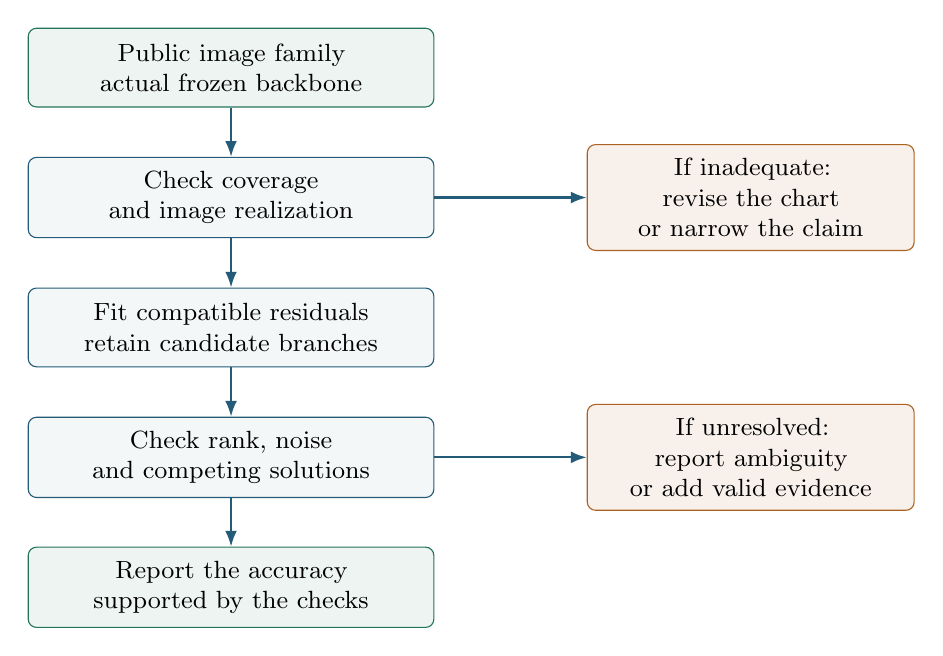
\begin{tikzpicture}
\node[learn,text width=4.8cm] (family) at (0,0) {Public image family\\actual frozen backbone};
\node[box,text width=4.8cm] (coverage) at (0,-1.65) {Check coverage\\and image realization};
\node[free,text width=3.8cm] (revise) at (6.6,-1.65) {If inadequate:\\revise the chart\\or narrow the claim};
\node[box,text width=4.8cm] (search) at (0,-3.3) {Fit compatible residuals\\retain candidate branches};
\node[box,text width=4.8cm] (test) at (0,-4.95) {Check rank, noise\\and competing solutions};
\node[free,text width=3.8cm] (uncertain) at (6.6,-4.95) {If unresolved:\\report ambiguity\\or add valid evidence};
\node[learn,text width=4.8cm] (claim) at (0,-6.6) {Report the accuracy\\supported by the checks};
\draw[arr] (family) -- (coverage);
\draw[arr] (coverage) -- (revise);
\draw[arr] (coverage) -- (search);
\draw[arr] (search) -- (test);
\draw[arr] (test) -- (uncertain);
\draw[arr] (test) -- (claim);
\end{tikzpicture}
\caption{A decision path for the programme. Each checkpoint answers a distinct question; failure at one is not repaired merely by improving the rendered image's appearance. The hierarchy accelerates the search step only when branch bounds actually exclude candidates.}
\label{fig:programme}
\end{figure}
\FloatBarrier

\begin{proposal}[A two-stage public atlas with image-consistent finishing]\label{pr:programme}
\textbf{First stage: a controlled feature result.} Extract public features from the exact frozen backbone and layer. Learn a modest feature autoencoder or a mixture of explicit chart decoders. Form a finite bank of local neighborhoods, including subject-specific and broader alternatives. Freeze the bank. Search compact certificate residuals and record local singular values. The point of this stage is a transparent test of span separation and public coverage, not merely a visually attractive decoder output.

\textbf{Second stage: realize and refine images.} Use a compatible public image decoder, or transfer the feature estimate to a frozen image-generator atlas. Re-optimize the image-side residual $C\Phi^0(G_j(z))$. Add other layers only with compatible feature maps and their drift error budgets. Add replay only when its forward training model is justified; use the certificate fiber as a reduced search domain under the constant-rank assumptions of Theorem~\ref{thm:compose}.

\textbf{Subject refinement.} Use text and rough outputs to select additional prebuilt chart families, retain competing identities, and inspect the normalized observation spectrum before unlocking more coordinates. Learn the selector from paired public adapter tasks only after the chart and residual pipeline is itself understood.

\textbf{Multiscale navigation.} Organize that same public bank as the hierarchy in Section~\ref{sec:multiscale}. Use region bounds that include approximation error, retain all branches not safely excluded, and compare search cost with the same charts searched without a hierarchy. Keep coverage, pruning efficiency, and final identifiability as separate questions.
\end{proposal}

\begin{center}
\small
\begin{longtable}{@{}Y{.23\textwidth}Y{.34\textwidth}Y{.33\textwidth}@{}}
\toprule
Question & Quantity or condition & What failure means\\
\midrule
\endhead
Does the chart cover this family? & Held-out sectional reconstruction; $\delta$ if the truth is available in a public task & The prior may be wrong even when the equation budget is ample\\[4pt]
Does the candidate have an image? & Exact image-side parameterization, or $\norm{\Phi^0(D_{\rm img}(\widehat h))-\widehat h}$ & A certified feature may be unrealizable\\[4pt]
Which coordinates are identified? & Rank and singular spectrum of the actual stacked Jacobian, normalized by chart geometry & Counts or sharp images cannot establish uniqueness\\[4pt]
Do deeper layers help? & Added independent tangent directions, actual perturbation bounds, and weighted bias & More rows can increase bias without useful information\\[4pt]
Is the brand supported? & Separation from competing feasible chart families under the observation & The brand may be supplied only by the prior\\[4pt]
Is a refinement valid? & Same fixed-atlas guarantee, or a declared adaptive validation argument & Selection can manufacture apparently consistent charts\\[4pt]
What can be claimed? & Local recovery bound plus coverage and alias exclusions & Otherwise report a plausible, compatible reconstruction\\
\bottomrule
\end{longtable}
\end{center}

\subsection{A short reading order, tied to decisions}

\begin{enumerate}
\item \textbf{Bora et al.~\cite{bora}:} understand the generative-prior inverse problem and representation-error term before claiming a new general chart principle.
\item \textbf{Alberti et al.~\cite{mixturevae}, then Schonsheck et al.~\cite{chartae}:} choose an explicit atlas architecture and understand why multiple coordinate patches matter.
\item \textbf{Har-Peled--Mendel~\cite{nettree}, Allard--Chen--Maggioni~\cite{gmra}, and Iwen et al.~\cite{onebitgmra}:} distinguish hierarchical metric navigation, multiscale local approximation, and recovery guarantees; identify what the LoRA observation model still requires.
\item \textbf{StyleGAN2~\cite{stylegan2} and GANSpace~\cite{ganspace}, or latent diffusion~\cite{ldm}:} choose an image expansion whose actual training domain matches the intended section; distinguish decoder coordinates from the restricted search.
\item \textbf{Pope et al.~\cite{pope}, Levina--Bickel~\cite{levina}, and Facco et al.~\cite{twonn}:} design scale-aware public dimension diagnostics.
\item \textbf{Ansuini et al.~\cite{ansuini} and Shao et al.~\cite{riemannian}:} compare layer geometry and normalize conditioning by actual image or feature changes.
\item \textbf{CLIP~\cite{clip} and retrieval-augmented diffusion~\cite{rdm}:} implement semantic proposals without confusing retrieval with evidence.
\item \textbf{Stanczuk et al.~\cite{stanczuk} and FLIPD~\cite{flipd}:} explore whether a pretrained diffusion prior can supply useful local tangent information.
\end{enumerate}

The practical object is an atlas whose construction and search account for the observation. Its public decoder supplies realistic detail; its patches control coverage; its hierarchy can reduce search when residual bounds exclude branches; and its observation Jacobian determines which local changes can be recovered. A progressively sharper prior-generated guess becomes a recovery claim only when coverage, conditioning, and the exclusion of competing explanations support it.

\section*{External mathematical input}
\addcontentsline{toc}{section}{External mathematical input}
The global fixed-chart theorem uses Sard's critical-value theorem, together with the standard constant-rank and regular-level-set theorems of differential calculus. The application to the constrained random kernel is proved in full in Theorem~\ref{thm:global}; it is not an assumption that the chart is generically positioned after seeing the release. Sard's original statement is available in \href{https://projecteuclid.org/journals/bulletin-of-the-american-mathematical-society/volume-48/issue-12/The-measure-of-the-critical-values-of-differentiable-maps/bams/1183504867.pdf}{Arthur Sard, \emph{The measure of the critical values of differentiable maps} (1942)}. A short account of the projection argument is also in \href{https://math.mit.edu/classes/18.965/2014FA/class3.pdf}{MIT's notes on parametric transversality}. The Gaussian residual, inverse-Gram, subspace-selection, and concentration statements used here have their proofs in the note. No literature-novelty claim is made for those tools or their applications.

\addcontentsline{toc}{section}{Primary-source references}
\renewcommand{\refname}{Primary-source references}
\begin{thebibliography}{99}
\small
\bibitem{bora}
A. Bora, A. Jalal, E. Price, and A. G. Dimakis.
\href{https://proceedings.mlr.press/v70/bora17a.html}{Compressed Sensing using Generative Models}.
ICML, PMLR 70, 2017.

\bibitem{mixturevae}
G. S. Alberti, J. Hertrich, M. Santacesaria, and S. Sciutto.
\href{https://jmlr.org/papers/v25/23-0396.html}{Manifold Learning by Mixture Models of VAEs for Inverse Problems}.
JMLR 25(202):1--35, 2024.

\bibitem{chartae}
S. Schonsheck, J. Chen, and R. Lai.
\href{https://arxiv.org/abs/1912.10094}{Chart Auto-Encoders for Manifold Structured Data}.
arXiv:1912.10094, 2019; revised 2020.

\bibitem{vae}
D. P. Kingma and M. Welling.
\href{https://arxiv.org/abs/1312.6114}{Auto-Encoding Variational Bayes}.
ICLR, 2014.

\bibitem{glo}
P. Bojanowski, A. Joulin, D. Lopez-Paz, and A. Szlam.
\href{https://arxiv.org/abs/1707.05776}{Optimizing the Latent Space of Generative Networks}.
ICML, 2018.

\bibitem{stylegan}
T. Karras, S. Laine, and T. Aila.
\href{https://arxiv.org/abs/1812.04948}{A Style-Based Generator Architecture for Generative Adversarial Networks}.
CVPR, 2019.

\bibitem{stylegan2}
T. Karras, S. Laine, M. Aittala, J. Hellsten, J. Lehtinen, and T. Aila.
\href{https://arxiv.org/abs/1912.04958}{Analyzing and Improving the Image Quality of StyleGAN}.
CVPR, 2020.

\bibitem{ganspace}
E. H\"ark\"onen, A. Hertzmann, J. Lehtinen, and S. Paris.
\href{https://arxiv.org/abs/2004.02546}{GANSpace: Discovering Interpretable GAN Controls}.
NeurIPS, 2020.

\bibitem{e4e}
O. Tov, Y. Alaluf, Y. Nitzan, O. Patashnik, and D. Cohen-Or.
\href{https://arxiv.org/abs/2102.02766}{Designing an Encoder for StyleGAN Image Manipulation}.
ACM Transactions on Graphics 40(4), 2021.

\bibitem{restyle}
Y. Alaluf, O. Patashnik, and D. Cohen-Or.
\href{https://arxiv.org/abs/2104.02699}{ReStyle: A Residual-Based StyleGAN Encoder via Iterative Refinement}.
ICCV, 2021.

\bibitem{ldm}
R. Rombach, A. Blattmann, D. Lorenz, P. Esser, and B. Ommer.
\href{https://arxiv.org/abs/2112.10752}{High-Resolution Image Synthesis with Latent Diffusion Models}.
CVPR, 2022.

\bibitem{clip}
A. Radford et al.
\href{https://proceedings.mlr.press/v139/radford21a.html}{Learning Transferable Visual Models From Natural Language Supervision}.
ICML, PMLR 139, 2021.

\bibitem{rdm}
A. Blattmann, R. Rombach, K. Oktay, J. M\"uller, and B. Ommer.
\href{https://proceedings.neurips.cc/paper_files/paper/2022/hash/62868cc2fc1eb5cdf321d05b4b88510c-Abstract-Conference.html}{Retrieval-Augmented Diffusion Models}.
NeurIPS, 2022.

\bibitem{unclip}
A. Ramesh, P. Dhariwal, A. Nichol, C. Chu, and M. Chen.
\href{https://arxiv.org/abs/2204.06125}{Hierarchical Text-Conditional Image Generation with CLIP Latents}.
arXiv:2204.06125, 2022.

\bibitem{dip}
D. Ulyanov, A. Vedaldi, and V. Lempitsky.
\href{https://openaccess.thecvf.com/content_cvpr_2018/html/Ulyanov_Deep_Image_Prior_CVPR_2018_paper.html}{Deep Image Prior}.
CVPR, 2018.

\bibitem{deepdecoder}
R. Heckel and P. Hand.
\href{https://arxiv.org/abs/1810.03982}{Deep Decoder: Concise Image Representations from Untrained Non-convolutional Networks}.
ICLR, 2019.

\bibitem{pope}
P. Pope, C. Zhu, A. Abdelkader, M. Goldblum, and T. Goldstein.
\href{https://arxiv.org/abs/2104.08894}{The Intrinsic Dimension of Images and Its Impact on Learning}.
ICLR, 2021.

\bibitem{ansuini}
A. Ansuini, A. Laio, J. H. Macke, and D. Zoccolan.
\href{https://arxiv.org/abs/1905.12784}{Intrinsic Dimension of Data Representations in Deep Neural Networks}.
NeurIPS, 2019.

\bibitem{levina}
E. Levina and P. J. Bickel.
\href{https://proceedings.neurips.cc/paper/2004/file/74934548253bcab8490ebd74afed7031-Paper.pdf}{Maximum Likelihood Estimation of Intrinsic Dimension}.
Advances in Neural Information Processing Systems 17, NIPS 2004.

\bibitem{twonn}
E. Facco, M. d'Errico, A. Rodriguez, and A. Laio.
\href{https://arxiv.org/abs/1803.06992}{Estimating the Intrinsic Dimension of Datasets by a Minimal Neighborhood Information}.
Scientific Reports 7:12140, 2017; author preprint posted 2018.

\bibitem{stanczuk}
J. Stanczuk, G. Batzolis, T. Deveney, and C.-B. Sch\"onlieb.
\href{https://arxiv.org/abs/2212.12611}{Your Diffusion Model Secretly Knows the Dimension of the Data Manifold}.
arXiv:2212.12611, 2022; revised 2023.

\bibitem{flipd}
H. Kamkari, B. L. Ross, R. Hosseinzadeh, J. C. Cresswell, and G. Loaiza-Ganem.
\href{https://arxiv.org/abs/2406.03537}{A Geometric View of Data Complexity: Efficient Local Intrinsic Dimension Estimation with Diffusion Models}.
NeurIPS, 2024.

\bibitem{riemannian}
H. Shao, A. Kumar, and P. T. Fletcher.
\href{https://arxiv.org/abs/1711.08014}{The Riemannian Geometry of Deep Generative Models}.
CVPR Workshops, 2018.
\bibitem{nettree}
S. Har-Peled and M. Mendel.
\href{https://epubs.siam.org/doi/10.1137/S0097539704446281}{Fast Construction of Nets in Low-Dimensional Metrics and Their Applications}.
SIAM Journal on Computing 35(5):1148--1184, 2006.

\bibitem{gmra}
W. K. Allard, G. Chen, and M. Maggioni.
\href{https://arxiv.org/abs/1105.4924}{Multiscale Geometric Methods for Data Sets II: Geometric Multi-Resolution Analysis}.
arXiv:1105.4924, 2011.

\bibitem{onebitgmra}
M. A. Iwen, F. Krahmer, S. Krause-Solberg, and J. Maly.
\href{https://arxiv.org/abs/1807.06490}{On Recovery Guarantees for One-Bit Compressed Sensing on Manifolds}.
arXiv:1807.06490, 2018; revised 2020.

\end{thebibliography}

\clearpage
\appendix
\section{Technical corrections to the supplied premises}\label{app:corrections}

\chapterbrief
{These corrections qualify the original formulations, not the goals of the project. They concern the score's domain, finite attainment of an affine optimum, survival of the initialization imprint, probability conditioning, and unjustified dimension counting. The main chapters use the corrected assumptions at each point of application.}
{Use this appendix as a checklist when quoting a theorem. The explicit failures are proved in Chapter~\ref{sec:counterexamples}; the generalized eigenproblem and probability convention are treated in Chapter~\ref{sec:certificate}.}
{$A=A_T$, $C=P_{\row(B_T)^\perp}A_T$, and $q<r\le n$. The scalar $\gamma$ below denotes the surviving initialization coefficient, not the fixed LoRA scale.}

The supplied exact certificate identity is an input to this note, not something re-derived here. Moving these qualifications to an appendix does not remove them from the theorem hypotheses.

\begin{correction}[The score has a domain]
Write $A=A_T$ and $P_\perp=P_{\row(B_T)^\perp}$. The score
\[
R(h)=\frac{\norm{Ch}^2}{\norm{Ah}^2},\qquad C=P_\perp A,
\]
is defined on $\mathcal D_A=\{h:Ah\ne0\}$. Its zero set is $\ker C\cap\mathcal D_A$, not all of $\ker C$. In particular, the zero representation and a possible training point with $Ah_i=0$ have undefined score. Throughout, zero-set theorems concern $C\psi$; their score versions require a nonzero denominator.
\end{correction}

\begin{correction}[The affine eigenvalue is an infimum]
The generalized eigenvalue is the infimum over the affine chart. It is attained at finite coordinates precisely when the lowest generalized eigenspace contains a vector whose first coordinate is nonzero. Otherwise the infimum is approached at infinity. Thus $\lambda_{\min}=0$ need not certify any finite chart point. The full proof is Proposition~\ref{prop:eigen}.
\end{correction}

\begin{correction}[The optimizer class needs a non-annihilation condition]
The stated optimizer class permits a scalar update that erases the surviving initialization component. Then $\rank B_T=q$ need not imply $\rank C=r-q$. For scalar dynamics admitting the usual imprint $C=\gamma P_{(A_0\HH)^\perp}A_0$, one must require $\gamma\ne0$, or directly assume the stated rank and kernel identities. Counterexample~\ref{ex:decay} gives two legitimate gradient steps with $\rank B_T=1<r=2$ but $C=0$.
\end{correction}

\begin{correction}[Ambient dimensions and probability conditioning]
The stated rank and dimension formulas require $q<r\le n$. Almost-sure consequences survive conditioning on any positive-probability valid-release event. Exact Gaussian distribution laws and quantitative tail probabilities do not automatically survive such conditioning: an event depending on the initialization can select atypical matrices. All probability laws are stated before that selection, with an explicit rule for conditioning on a valid release.
\end{correction}

\begin{correction}[Inversion is not universally underdetermined]
A released full gradient or endpoint can have more independent local measurements than the candidate data have coordinates. Nonuniqueness must be established from a fiber or a Jacobian, not asserted from the fact that inputs are images. Likewise, the proposed capacity line involving image count is not used here and is not converted into a theorem by substituting $q$.
\end{correction}
\end{document}
